\section{Resultate des Messaufbaus}
In diesem Kapitel werden die Messresultate des Laboraufbaus analysiert und mit den Werten der Simulationen und den Normen verglichen. Hierbei wurden die Daten der Messungen als .csv Datei gespeichert, um mit Matlab die Signale schön darstellen zu können und das FFT berechnen zu können. 
Zudem befinden sich in diesem Kapitel nur die Messungen des Widerstandes und der ASM welche in Stern geschaltet sind. Die Messungen in Dreieckschaltung wurden gemacht aber nicht hier aufgeführt, da dies den Rahmen dieses Kapitels sprengen würde. Die Dreiecksmessungen befinden sich als Matlabdateien digital auf dem USB-Stick. \todo{angeben ob als USB Stick/CD oder sonst abgegeben}

\subsection{Messungen Ströme}
Um die Messungen mit den Normen vergleichen zu können, wurden die Ströme bei den verschiedenen Ansteuerungsarten gemessen. Von den gemessenen Signalen wurde anschliessend das FFT mit Matlab gemacht. 

\subsubsection{Messungen Widerstand}
Weil durch den Widerstand keine \SI{16}{A} Effektivstrom durchgelassen werden können, da der Widerstand bei \SI{150}{\Omega} nur bis zu \SI{2.4}{A} verträgt, mussten die gemessenen Werte auf \SI{16}{A} hochgerechnet werden. Von den berechneten Werten wird ebenfalls das FFT mit Matlab gemacht und die Amplituden können mit den Normen verglichen werden. Dazu wurden die Werte der Oberschwingungsordungen des FFTs in eine Tabelle aufgetragen. Falls die die Amplituden der Oberschwingungsordnungen sehr klein und diese für den Vergleich nicht geeignet sind, wurden Amplituden der Sub- und Zwischenharmonischen in der Tabelle aufgetragen.

\subsubsection*{Phasenanschnitt 60\textdegree}

\begin{figure}[ht!]
	\centering
	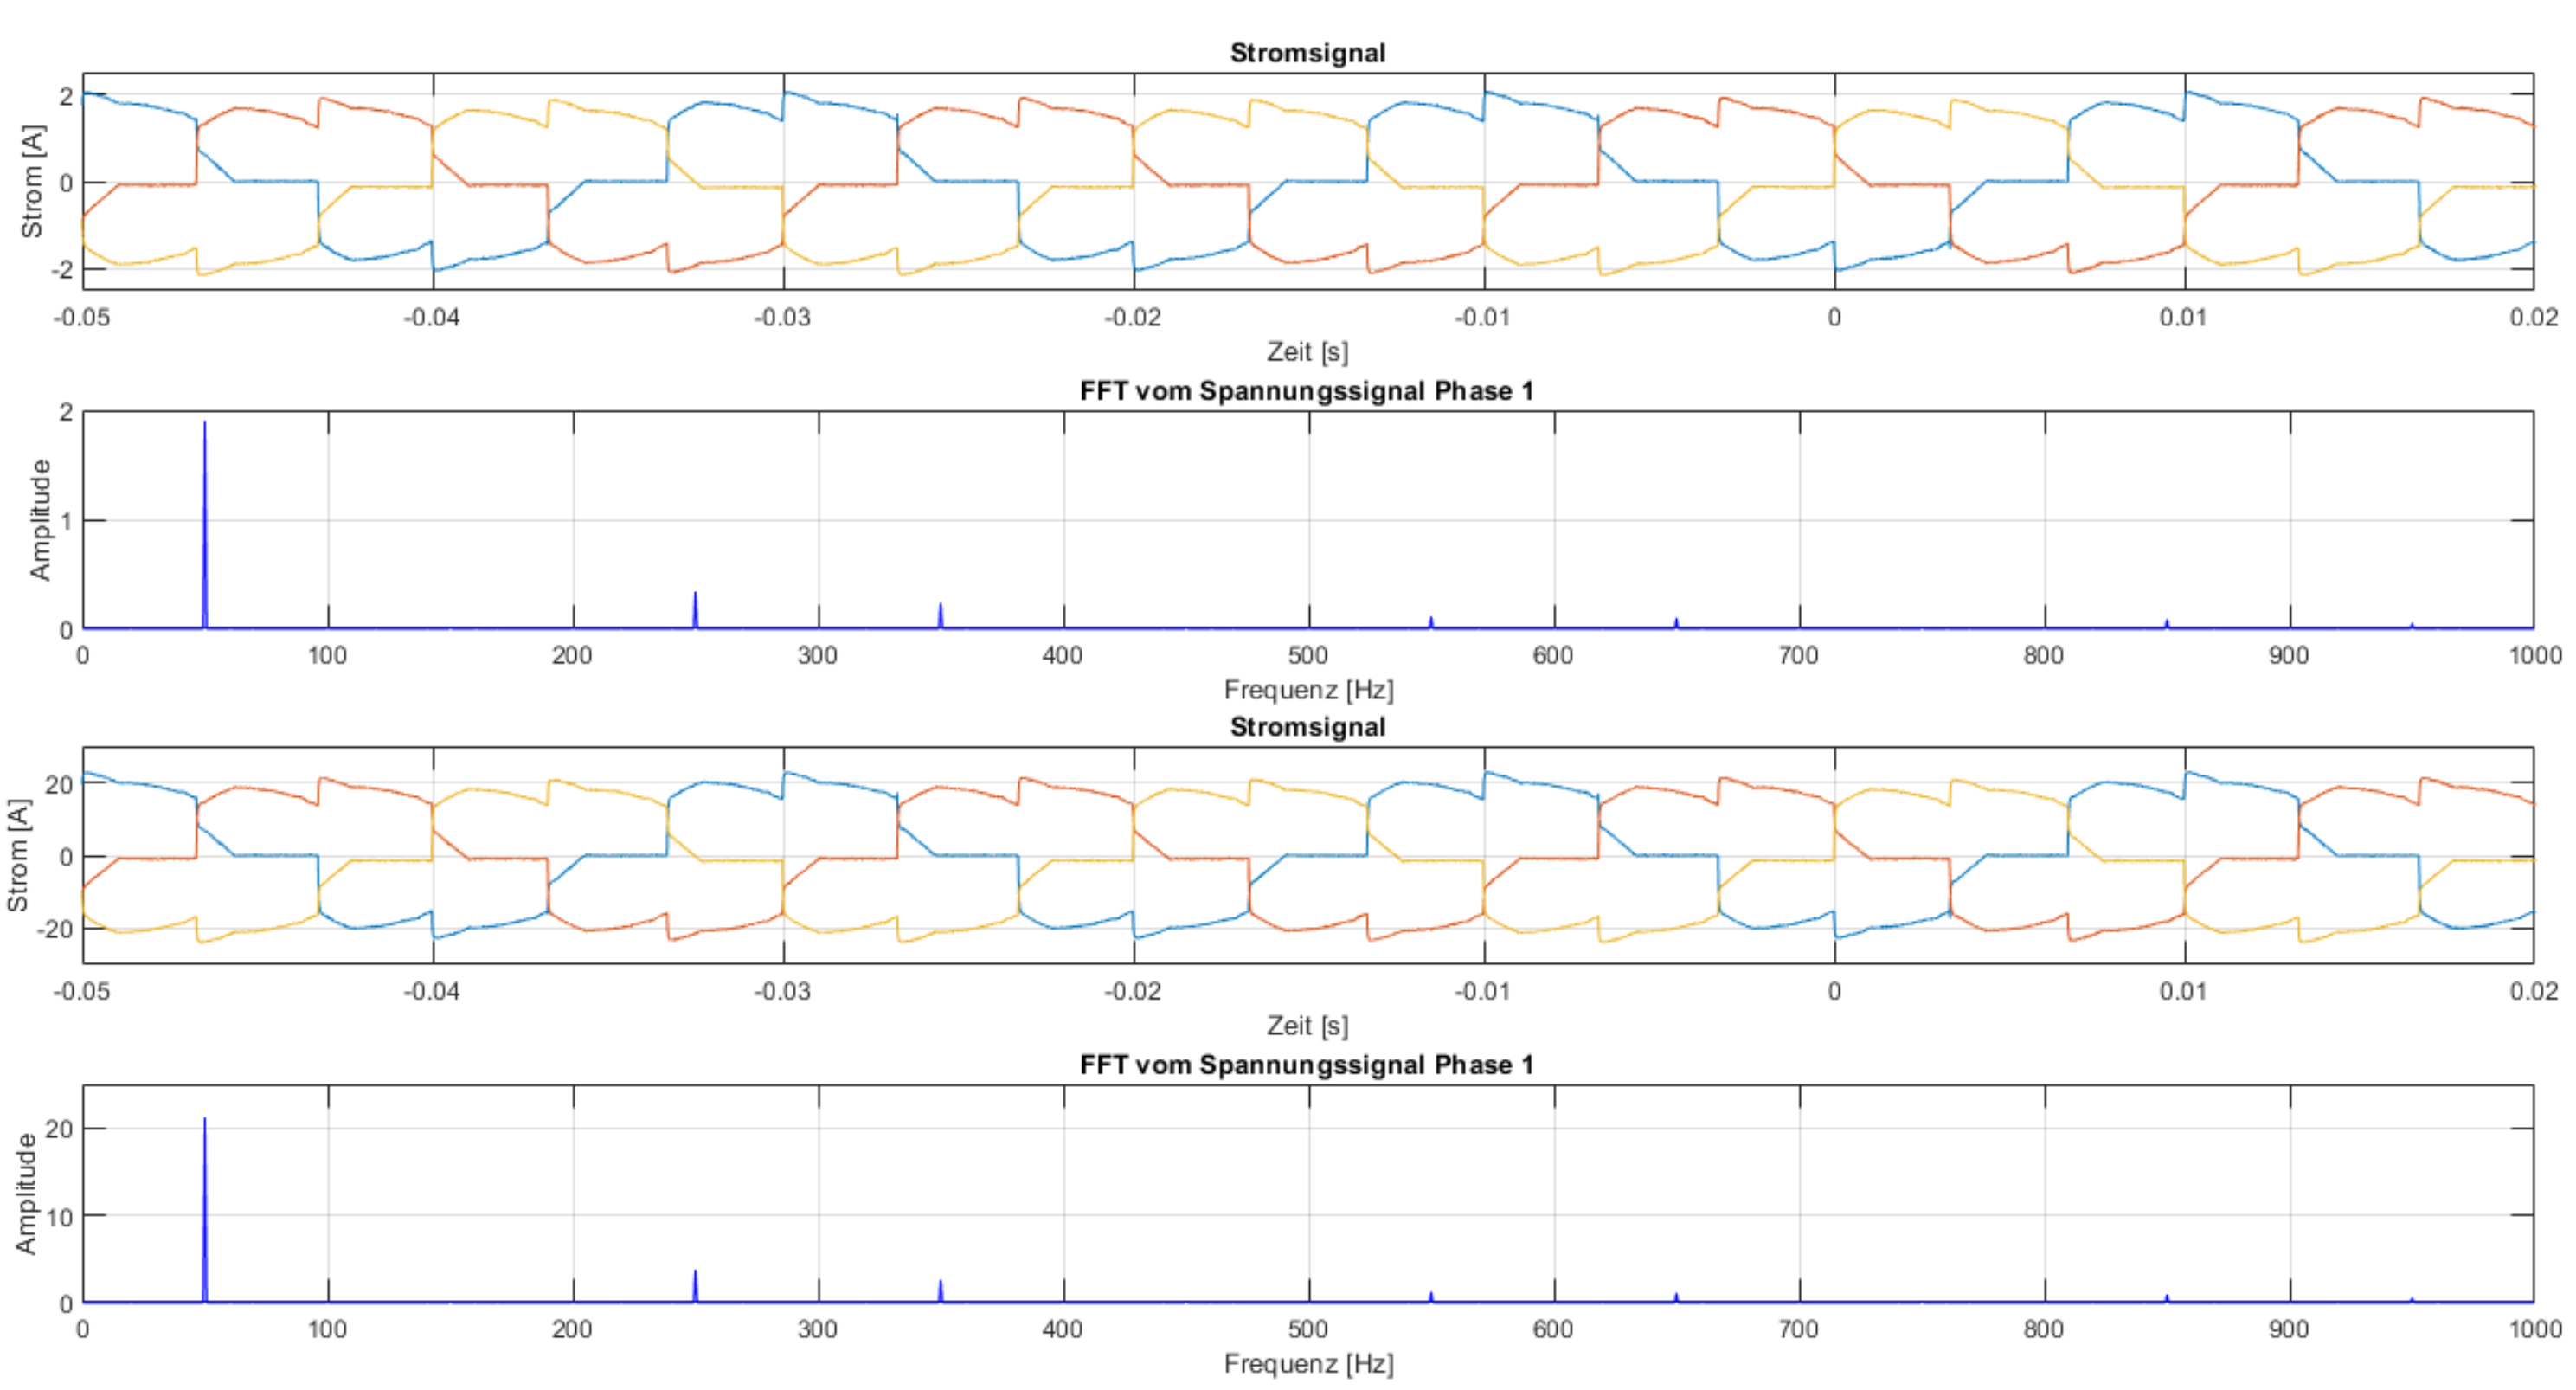
\includegraphics[width=\textwidth]{Messung_Widerstand_Phas_60grad_stroeme.png}	
	\caption{Messung mit Phasenanschnitt 60\textdegree}\label{fig:Mess_Widerstand_Phas_60grad_stroeme}
\end{figure}

Auf der Abbildung \ref{fig:Mess_Widerstand_Phas_60grad_stroeme} ist ersichtlich, dass bei den Oberschwingungsordnungen 3, 9 und 15 die Amplitude 0 ist, deswegen wurde diese nicht in der Tabelle \ref{tab:Phas_90_Stroeme} aufgeführt.

\begin{table}[ht!]
	\centering
	\begin{tabular}{|l|l|l|}
		\hline
		Oberschwingungsordnung & Amplitude [A] 	& Verhältnis zur Grundschwingung	\\ \hline
		1                      & 21.1996   		& 100\%								\\ \hline
		5                      & 3.7851    		& 17.86\%							\\ \hline
		7                      & 2.6127    		& 12.32\%							\\ \hline
		11                     & 1.2267    		& 5.79\%							\\ \hline
	\end{tabular}
	\caption{Amplitudenwerte bei den harmonischen Oberschwingungen bei Phasenanschnitt 60\textdegree}\label{tab:Phas_60_Stroeme}
\end{table}
%Die Höhe der Amplituden der Oberschwingungen der Tabelle \ref{tab:Phas_60_Stroeme} können mit den Normen in der Tabelle \ref{tab:Grenzwerte_Normen} verglichen werden. Dabei wird festgestellt, dass die Werte der Messung höher sind als die Normen zulassen.

Wenn die Werte der Messungen in der Tabelle \ref{tab:Phas_60_Stroeme} mit der Werte der Normen in der Tabelle \ref{tab:Grenzwerte_Normen} verglichen werden, ist ersichtlich, dass die Amplituden bei der Oberschwingungsordung 5 bis 19 zu hoch sind. So kann gesagt werden, dass sich der Phasenanschnitt mit 60\textdegree \hspace{0.02cm} nicht eignet um Widerstände anzusteuern, da diese nicht den Normen entsprechen. 


\subsubsection*{Phasenanschnitt 90\textdegree}
\begin{figure}[ht!]
	\centering
	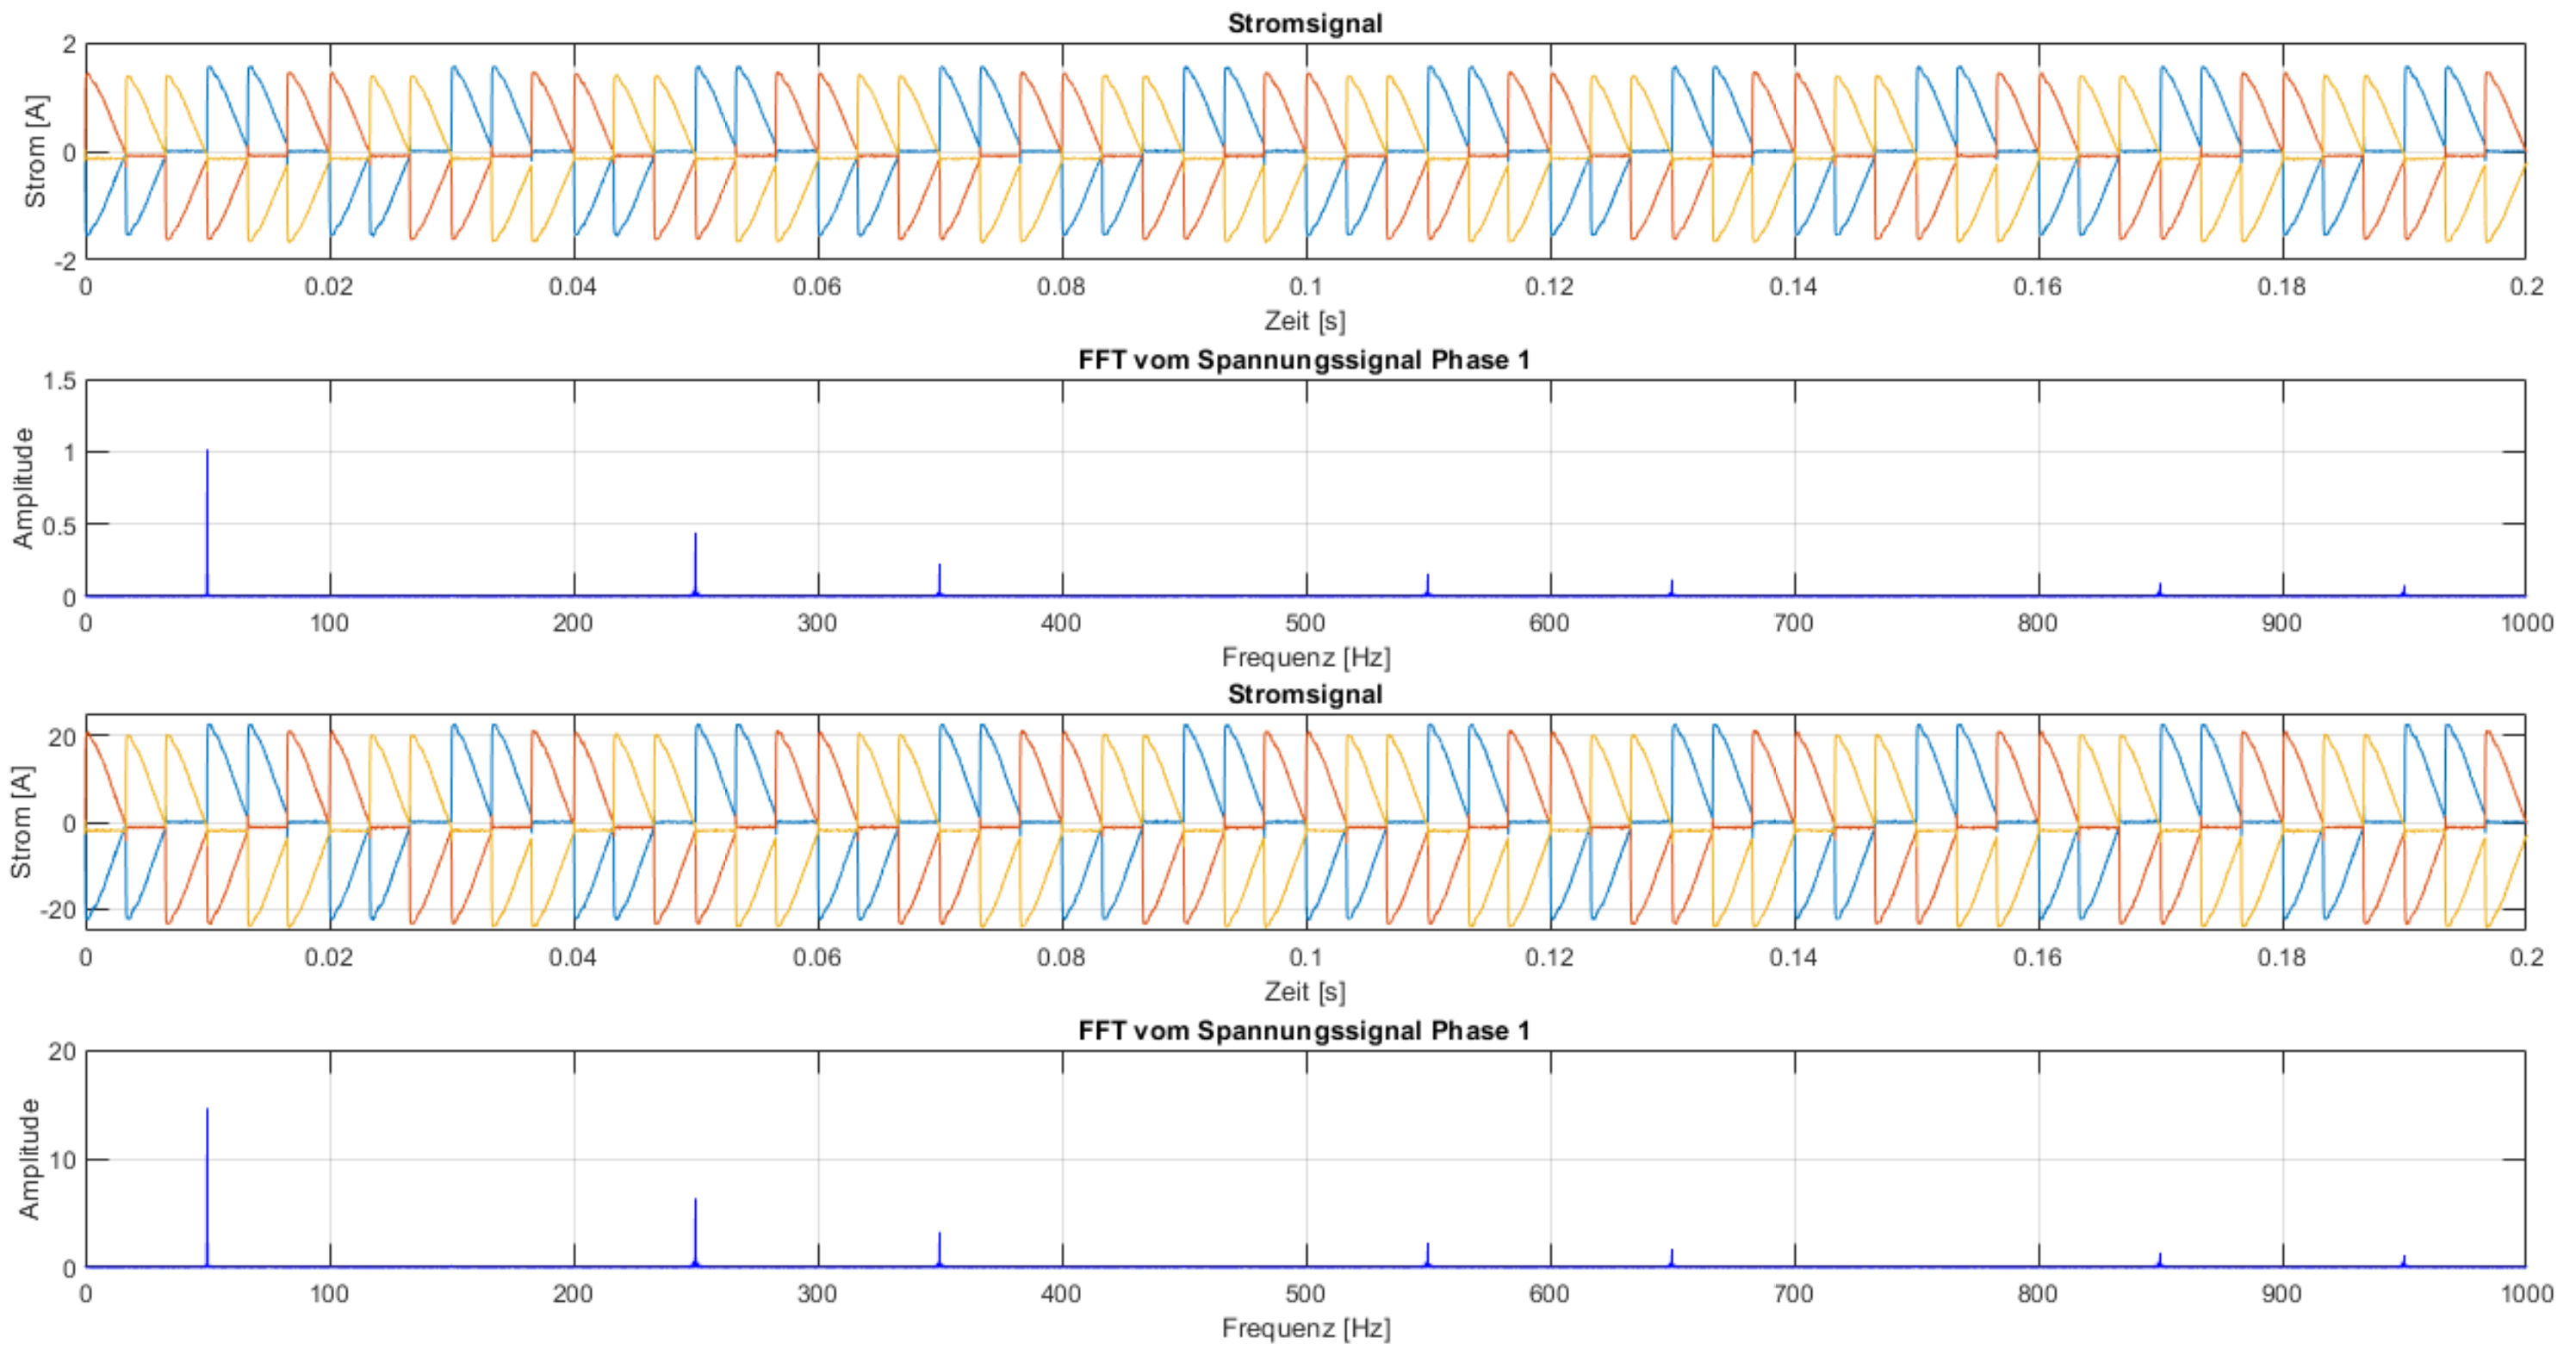
\includegraphics[width=\textwidth]{Messung_Widerstand_Phas_90grad_stroeme.png}	
	\caption{Phasenanschnitt 90\textdegree}\label{fig:Mess_Widerstand_Phas_90grad_stroeme}
\end{figure}

\begin{table}[ht!]
	\centering
	\begin{tabular}{|l|l|l|}
		\hline
		Oberschwingungsordnung 	& Amplitude [A] & Verhältnis zur Grundschwingung	\\ \hline
		1       				& 14.647   		& 100\%								\\ \hline
		5      					& 6.3481    	& 43.34\%							\\ \hline
		7      					& 3.2571    	& 22.24\%							\\ \hline
		11      				& 2.273    		& 15.52\%							\\ \hline
	\end{tabular}
	\caption{Amplitudenwerte bei den harmonischen Oberschwingungen bei Phasenanschnitt 90\textdegree}\label{tab:Phas_90_Stroeme}
\end{table}

Wie auch beim Phasenanschnitt mit 60\textdegree, befinden sich die Werte der Oberschwingungen, in der Tabelle \ref{tab:Phas_90_Stroeme} deutlich über den erlaubten Grenzwerten der Normen. Somit eignet sich auch der Phasenanschnitt mit 90\textdegree \hspace{0.02cm} nicht, Widerstände anzusteuern. 

%Wenn die Werte mit der Werte der Tabelle \ref{tab:Grenzwerte_Normen} verglichen werden, ist ersichtlich, dass die Amplituden bei der Oberschwingungsordung 5 bis 19 zu hoch sind. So kann gesagt werden, dass sich der Phasenanschnitt mit 90\textdegree \hspace{0.02cm} nicht eignet um Widerstände anzusteuern, da diese nicht den Normen entsprechen. Auf der Abbildung \ref{fig:Mess_Widerstand_Phas_90grad_stroeme} ist ersichtlich, dass bei den Oberschwingungsordnungen 3, 9 und 15 die Amplitude 0 ist, deswegen wurde diese nicht in der Tabelle \ref{tab:Phas_60_Stroeme} aufgeführt.


\newpage
\subsubsection*{Hartes Auf- und Absteuern}
\begin{figure}[ht!]
	\centering
	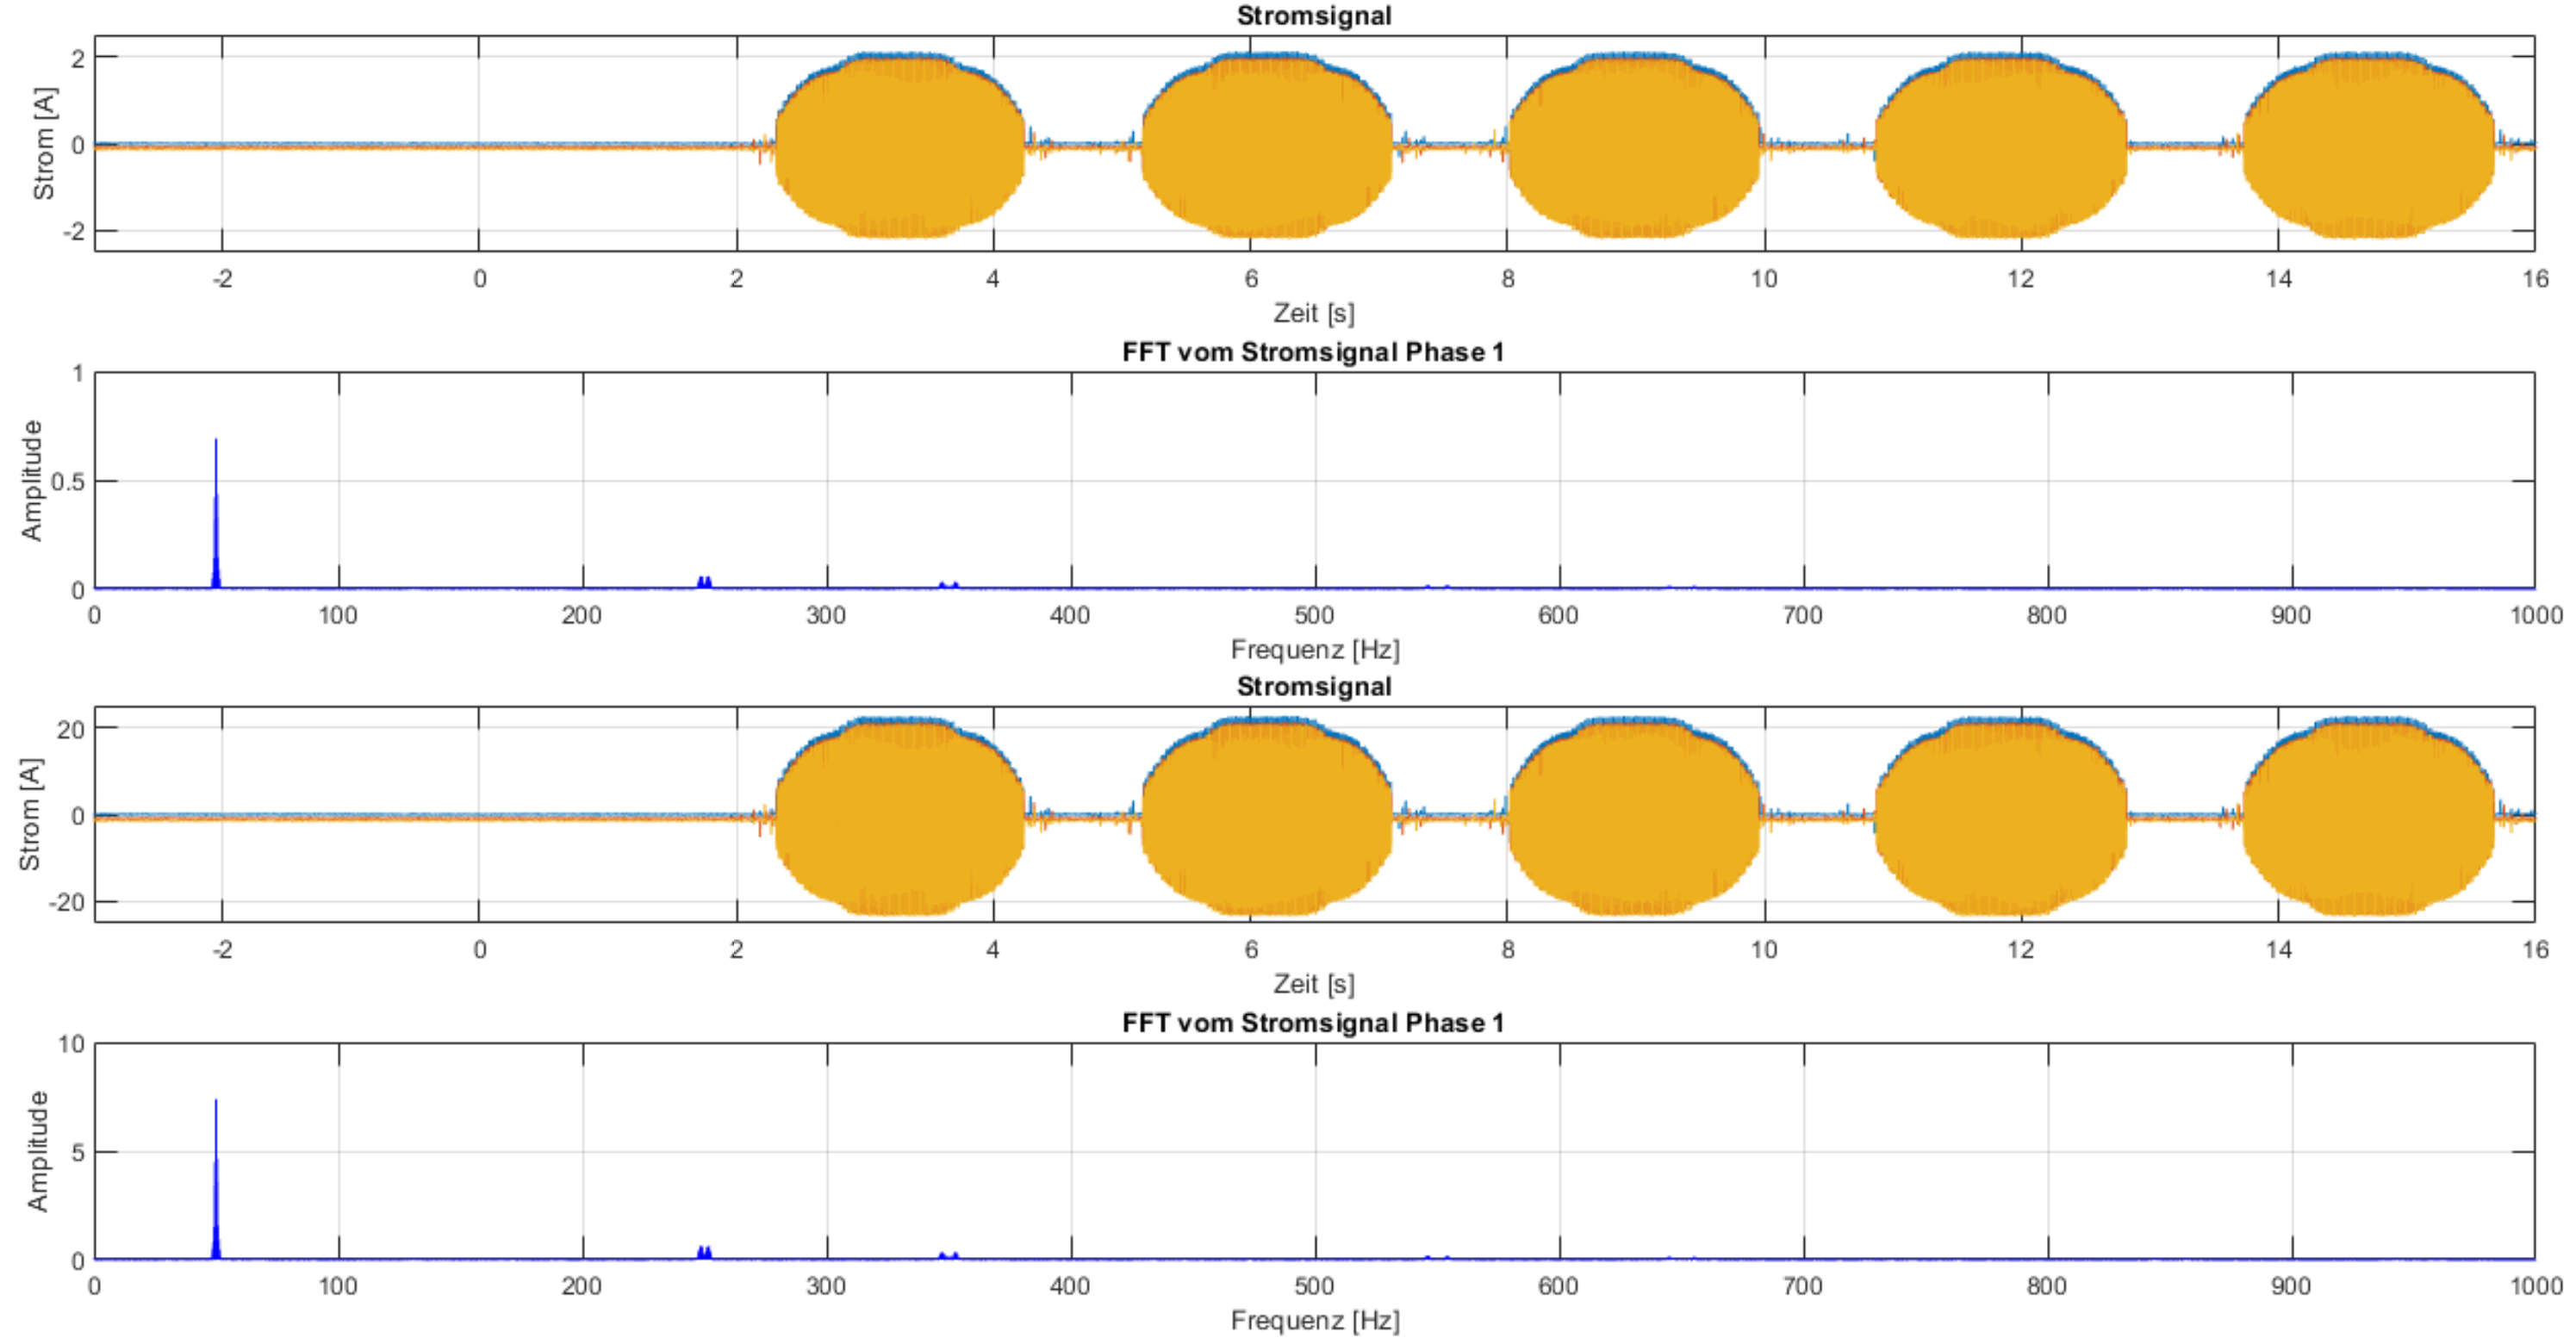
\includegraphics[width=\textwidth]{Messung_Widerstand_Sanft_stroeme.png}	
	\caption{Messung mit Auf- und Absteuern}\label{fig:Mess_Widerstand_Sanft_stroeme}
\end{figure}
Da beim hartem Auf- und Absteuern bereits ab der fünften Harmonischen die Amplitude unter \SI{0.1}{A} sind, wurde darauf verzichtet diese Tabellarisch aufzulisten. Jedoch sind bei dieser Messung die Sub- und Zwischenharmonische sehr interessant. Diese sind in der Tabelle \ref{tab:Sanft_stroeme} aufgeführt.

\begin{table}[ht!]
	\centering
	\begin{tabular}{|l|l|l|}
		\hline
		Frequenz {[}Hz{]} & Amplitude {[}A{]} & Verhältnis zur Grundschwingung	\\ \hline
		49.3              & 1.5146            & 20.51\%							\\ \hline
		49.6              & 4.4853            & 60.73\%							\\ \hline
		49.7              & 2.618             & 35.45\%							\\ \hline
		50                & 7.3857            & 100\%							\\ \hline
		50.05             & 3.73              & 50.5\%							\\ \hline
		50.35             & 4.662             & 63.12\%							\\ \hline
		50.7              & 1.5504            & 21\%							\\ \hline
		248.65            & 0.6226            & 8.43\%							\\ \hline
		250               & 0.0883            & 1.2\%							\\ \hline
		251.45            & 0.6               & 8.12\%							\\ \hline
	\end{tabular}
	\caption{Amplitudenwerte bei verschiedenen Frequenzen beim hartem Auf- und Absteuern}\label{tab:Sanft_stroeme}
\end{table}

Es ist ersichtlich, dass die Werte der Sub- und Zwischenharmonischen um \SI{50}{Hz}, mehr als der Hälfte der Grundschwingung entsprechen. Diese Trägerbänder existieren auch um die harmonischen Oberwellen, sind jedoch sehr klein. Im Vergleich mit den Normen kann gesagt werden, dass das harte Auf- und Absteuern unterhalb der erlaubten Grenzwerte liegt.


\newpage
\subsubsection*{Sanftes Auf- und Absteuern}\label{sec:Sanft_Widerstand_stroeme}
\begin{figure}[ht!]
	\centering
	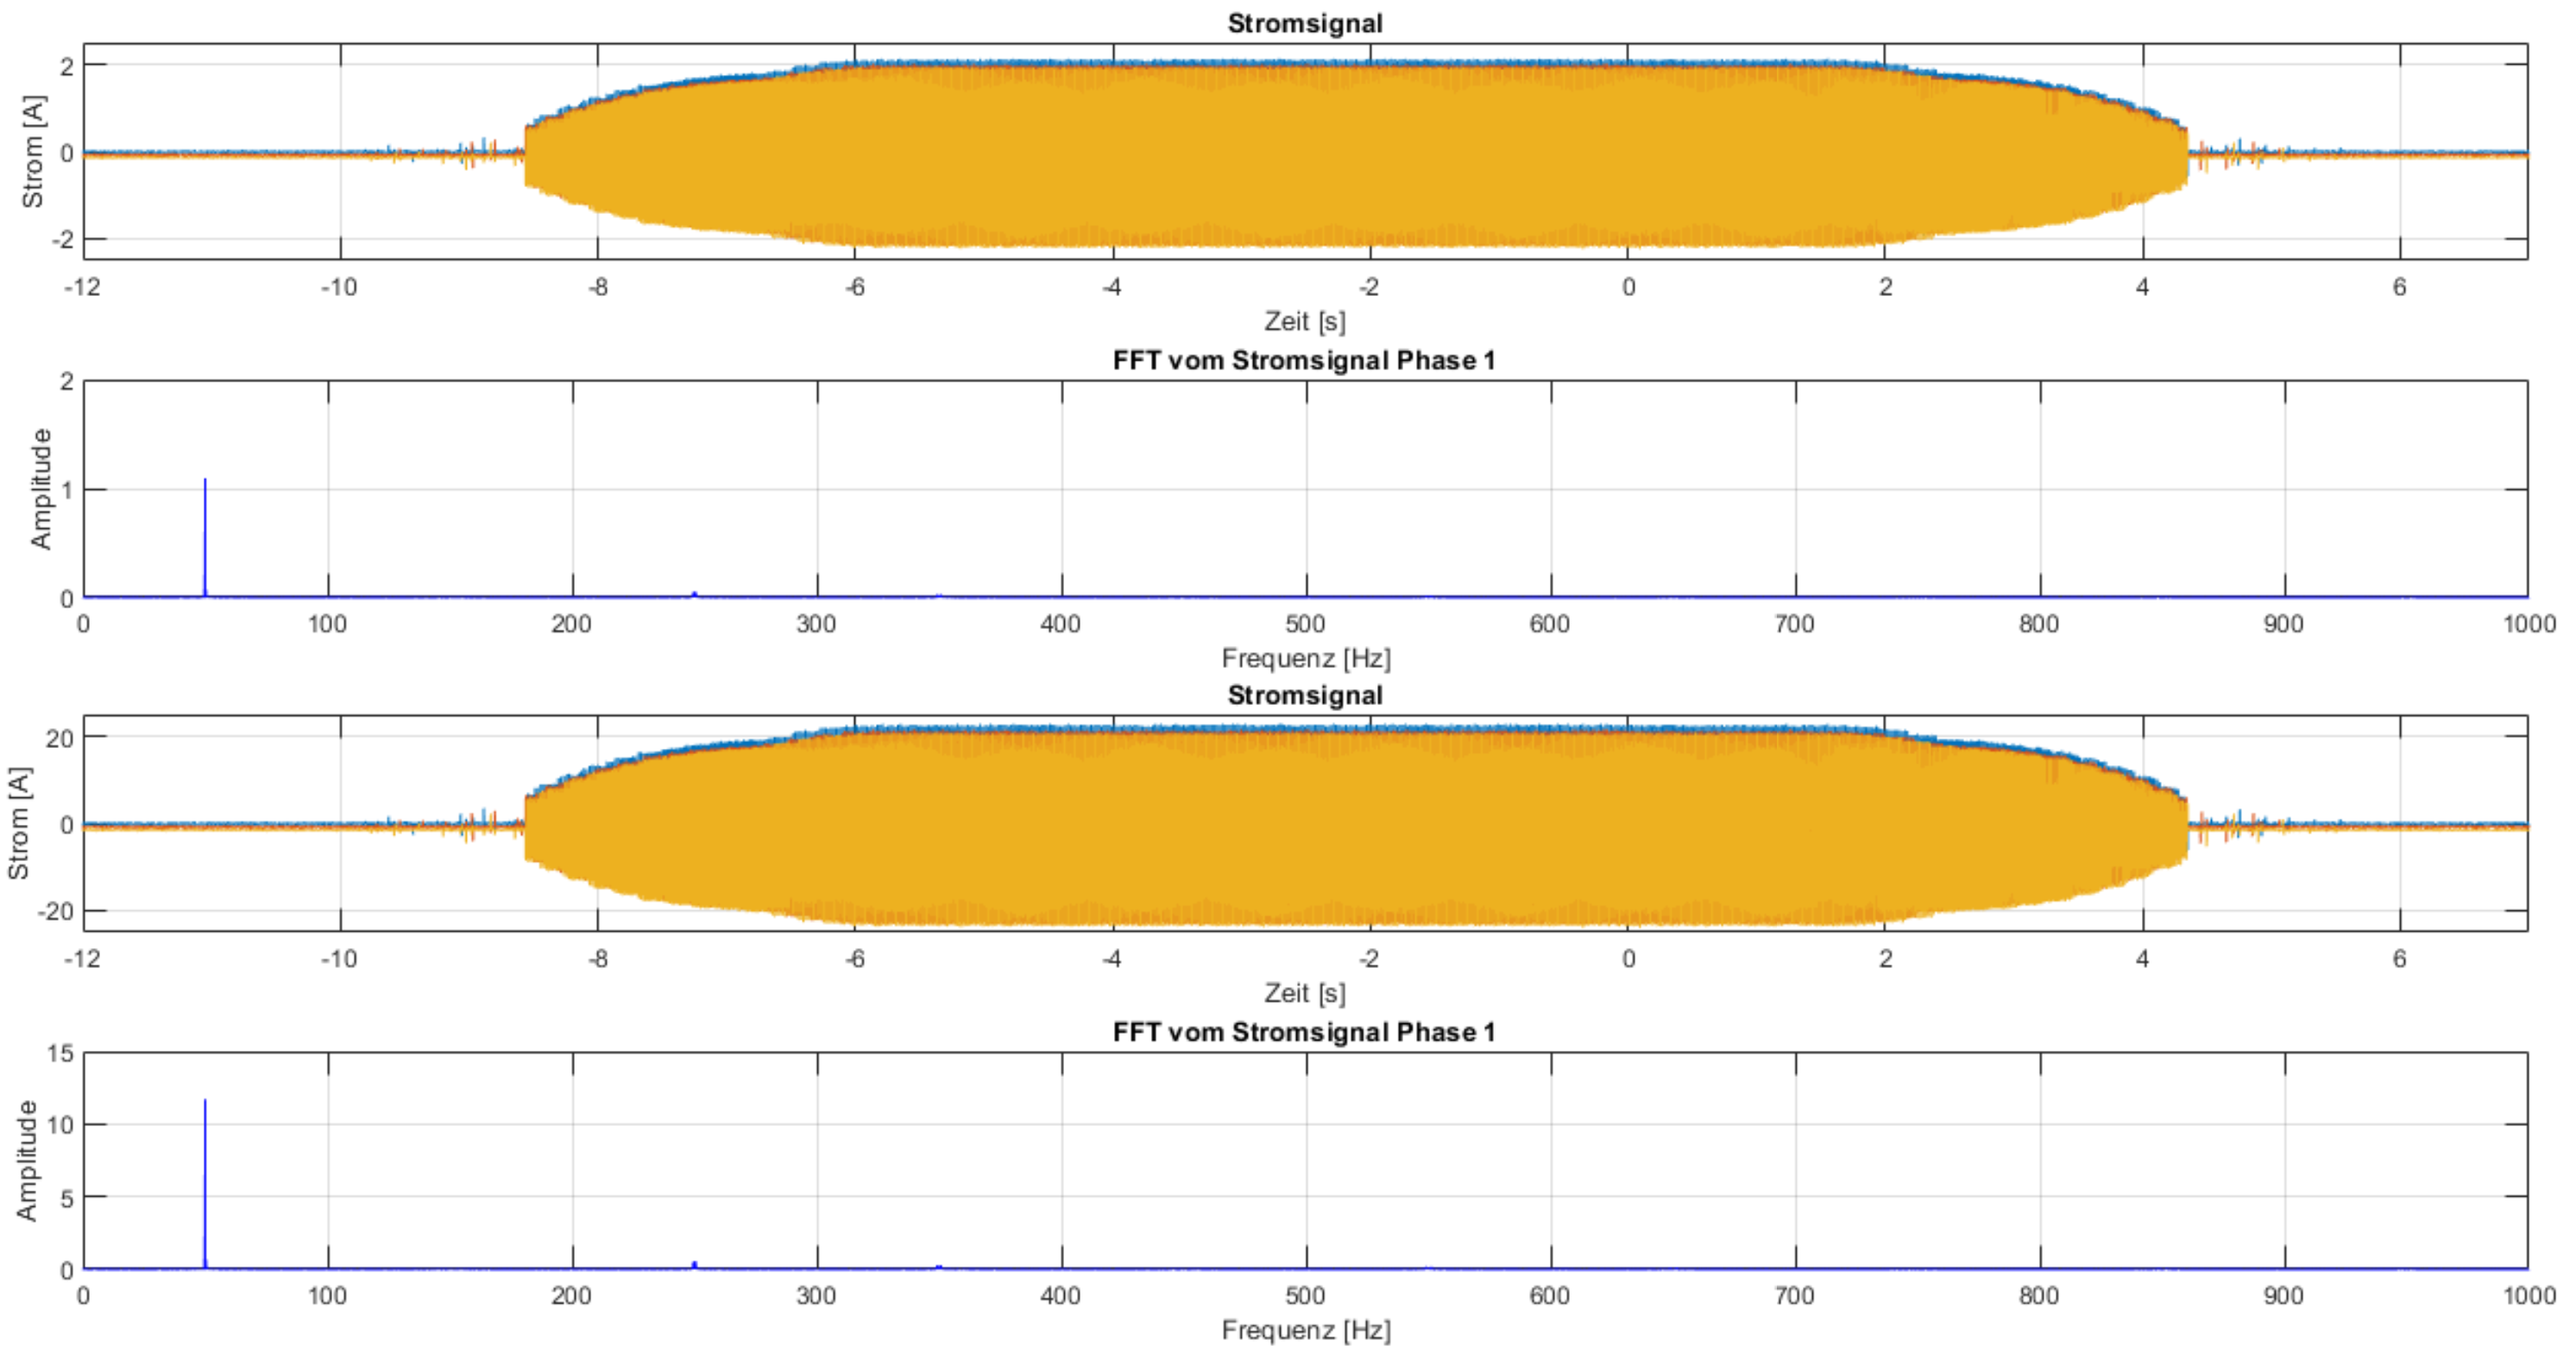
\includegraphics[width=\textwidth]{Messung_Widerstand_Sanft_langsam_stroeme.png}	
	\caption{Messung mit sanftem Auf- und Absteuern}\label{fig:Mess_Widerstand_Sanft_langsam_stroeme}
\end{figure}

Wie auch beim hartem Auf- und Absteuern, sind beim sanftem Auf- und Absteuern fast keine harmonische Oberwellen vorhanden. Die Amplitude der Grundschwingung ist höher als beim harten Auf- und Absteuern. Dies hat den Grund, dass länger auf der vollen Leistung gefahren wird. Weil beim sanften Auf- und Absteuern langsamer hoch- und runtergefahren wird, ist das Trägerband um \SI{50}{Hz} kleiner. Dies zeigt auch schon der visuelle Vergleich der Abbildungen \ref{fig:Mess_Widerstand_Sanft_langsam_stroeme} und \ref{fig:Mess_Widerstand_Sanft_stroeme}.

\begin{table}[ht!]
	\centering
	\begin{tabular}{|l|l|l|}
		\hline
		Frequenz {[}Hz{]} & Amplitude {[}A{]} & Verhältnis zur Grundschwingung	\\ \hline
		49.8              & 1.148             & 9.8\%							\\ \hline
		49.85             & 1.786             & 15.25\%							\\ \hline
		49.9              & 1.519             & 12.97\%							\\ \hline
		49.95             & 6.703             & 57.22\%							\\ \hline
		50                & 11.715            & 100\%							\\ \hline
		50.05             & 7.136             & 60.91\%							\\ \hline
		50.1              & 1.473             & 12.57\%							\\ \hline
		50.15             & 1.923             & 16.41\%							\\ \hline
		249.65            & 0.563             & 4.81\%							\\ \hline
		250               & 0.186             & 1.59\%							\\ \hline
		250.35            & 0.559             & 4.77\%							\\ \hline
	\end{tabular}
	\caption{Amplitudenwerte bei den harmonischen Oberschwingungen bei sanftem Auf- und Absteuern}\label{tab:Sanft_langsam_stroeme}
\end{table}

Im Vergleich zum hartem Auf- und Absteuern, ist die fünfte Harmonische 0.39\% grösser, welches einem sehr kleinem Unterschied entspricht. Jedoch sind die Peaks der Trägerbänder näher bei \SI{50}{Hz}. Die Peaks des Trägerbandes bei \SI{250}{Hz} sind im Verhältnis zur Grundschwingung, bei dem sanften Auf- und Absteuern kleiner als beim hartem Auf- und Absteuern.



\newpage
\subsubsection{Messungen ASM}
Für die Strommessungen mit der ASM wurde mit dem Phasenanschnitt und mit dem sanften Auf- und Absteuern gemessen. Dies hat den Grund, dass keine Anwendung für das harte Auf- und Absteuern oder die Schwingungspaketsteuerung gefunden wurde. Ausserdem wird in der Praxis meistens der Phasenanschnitt verwendet. Wie auch schon beim Widerstand muss der Strom bei der ASM auf die \SI{16}{A} hochgerechnet werden, um diese mit der Norm vergleichen zu können.
\subsubsection*{Phasenaschnitt 60\textdegree}
\begin{figure}[ht!]
	\centering
	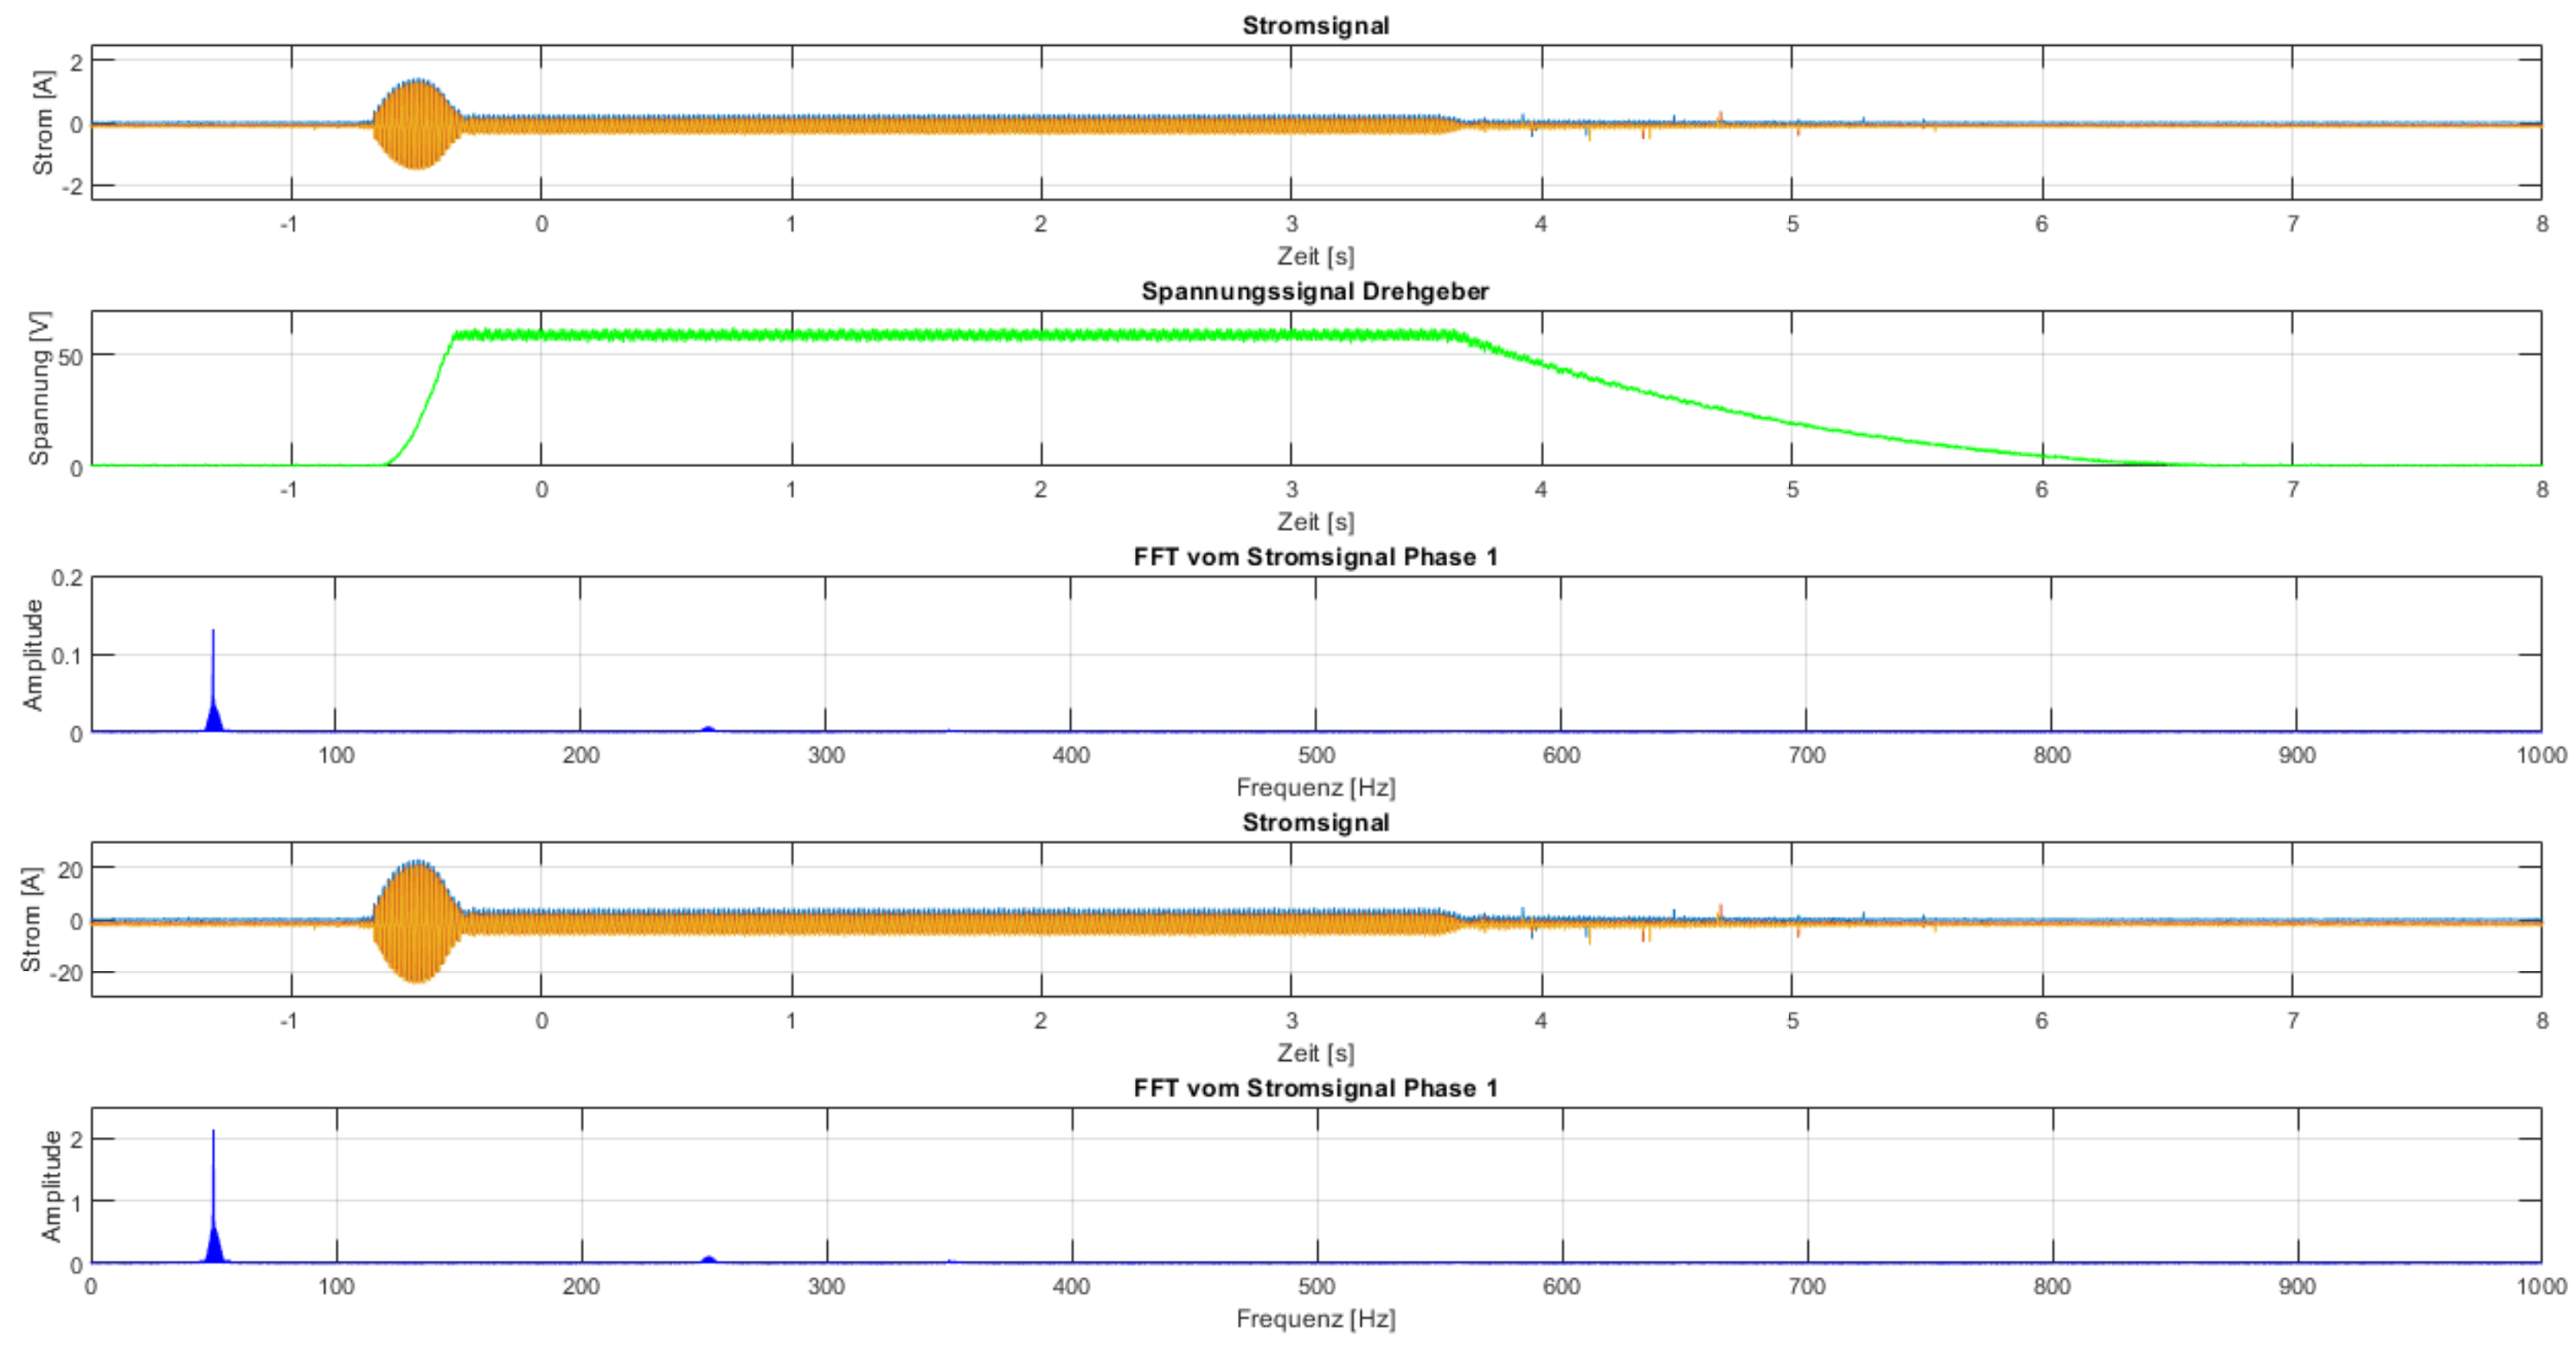
\includegraphics[width=\textwidth]{Messung_ASM_Phas_60grad_stroeme.png}	
	\caption{Messung mit Phasenanschnitt 60\textdegree}\label{fig:Mess_Phas_60grad_stroeme}
\end{figure}
Entgegen den Vorkenntnissen bei Phasenanschnitt mit einem Winkel von 60\textdegree, gibt es bei der Ansteuerung der ASM praktisch keine Harmonischen Oberwellen sondern Sub- und Zwischenharmonische. Dies hat den Grund, dass die Maschine auf die maximale Drehzahl fährt und so ist in der Maschine ein ungestörter Sinus mit einer Frequenz von \SI{50}{Hz}.

\begin{table}[ht!]
	\centering
	\begin{tabular}{|l|l|l|}
		\hline
		Frequenz {[}Hz{]} & Amplitude {[}A{]} & Verhältnis zur Grundschwingung	\\ \hline
		49.7              & 0.76              & 35.53\%							\\ \hline
		49.9              & 1.317             & 61.57\%							\\ \hline
		50                & 2.139             & 100\%							\\ \hline
		50.1              & 1.53              & 71.53\%							\\ \hline
		50.3              & 0.675             & 31.56\%							\\ \hline
		250               & 0.07              & 3.27\%							\\ \hline
	\end{tabular}
	\caption{Amplitudenwerte bei den harmonischen Oberschwingungen bei Phasenanschnitt 60\textdegree}\label{tab:Phas_60_ASM_stroeme}
\end{table}

Die fünfte Harmonische entspricht im FFT nur 3.27\% der Grundschwingung und ist so klein. Die Peaks des Trägerbandes um die Grundschwingung sind im Verhältnis mit bis zu 70\% sehr hoch.

\newpage
\subsubsection*{Phasenaschnitt 90\textdegree}
\begin{figure}[ht!]
	\centering
	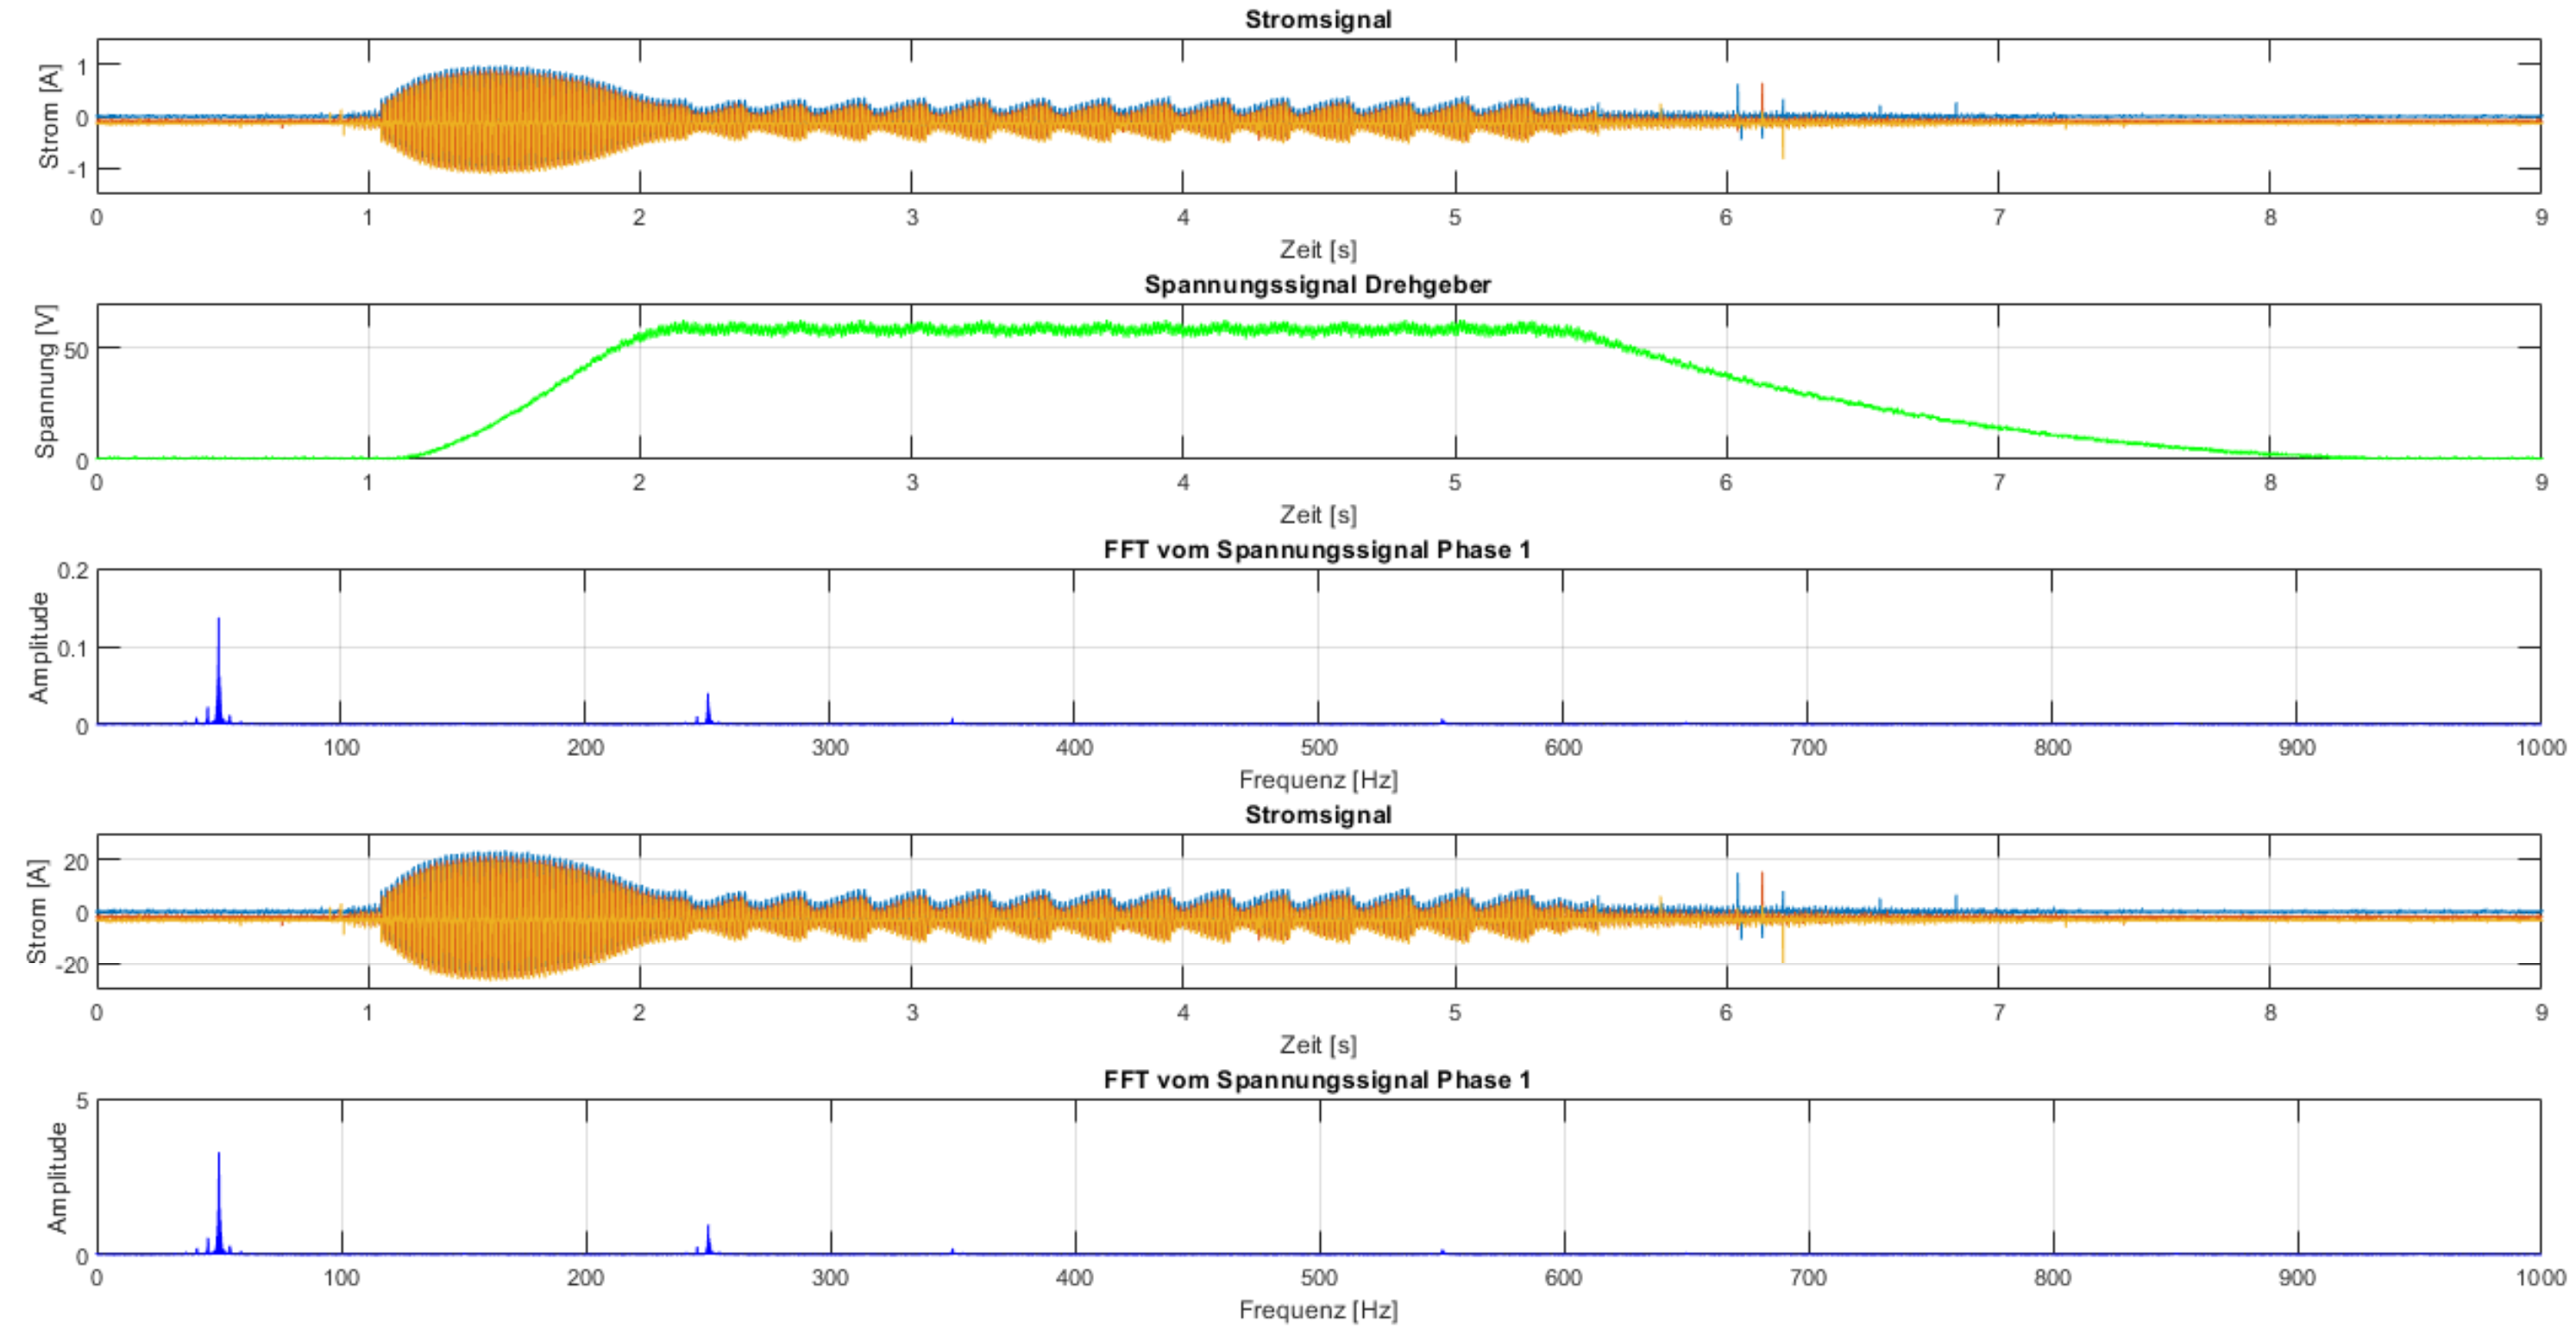
\includegraphics[width=\textwidth]{Messung_ASM_Phas_90grad_stroeme}	
	\caption{Messung mit Phasenanschnitt 90\textdegree}\label{fig:Mess_Phas_90grad_stroeme}
\end{figure}
Anders als bei der Ansteuerung mit dem Phasennaschnitt von 60\textdegree, treten mit 90\textdegree \hspace{0.02cm} bei der fünften Harmonischen grössere harmonische Oberwellen auf. Zusätzlich sind auch die Sub- und Zwischenharmonischen grösser als bei 60\textdegree. Auf der Abbildung \ref{fig:Mess_Phas_60grad_stroeme} ist beim Stromsignal ersichtlich, dass die Maschine schwingt. Dies wurde auch beim Testen festgestellt, dass die ASM nicht konstant auf der gleichen Drehzahl drehte.  
\begin{table}[ht!]
	\centering
	\begin{tabular}{|l|l|l|}
		\hline
		Frequenz {[}Hz{]} & Amplitude {[}A{]} & Verhältnis zur Grundschwingung	\\ \hline
		49.7              & 1.399             & 42.6\%							\\ \hline
		49.9              & 2.023             & 61.61\%							\\ \hline
		50                & 3.2839            & 100\%							\\ \hline
		50.1              & 2.567             & 78.17\%							\\ \hline
		50.3              & 1.468             & 44.71\%							\\ \hline
		250               & 0.673             & 20.5\%							\\ \hline
		250.1             & 0.959             & 29.2\%							\\ \hline
		250.2             & 0.687             & 20.92\%							\\ \hline
	\end{tabular}
	\caption{Amplitudenwerte bei den harmonischen Oberschwingungen bei Phasenanschnitt 90\textdegree}\label{tab:Phas_90_ASM_stroeme}
\end{table}

Im Vergleich zum Phasenanschnitt mit 60\textdegree, sind die Peaks des Trägerbandes um die Grundschwingung noch höher. Auch die fünfte Harmonische entspricht im Verhältnis zur Grundschwingung 20.5\%. Die Amplitude jedoch ist immer noch kleiner als der erlaubte Grenzwert der Norm. 


\newpage
\subsubsection*{Sanftes Auf- und Absteuern}
\begin{figure}[ht!]
	\centering
	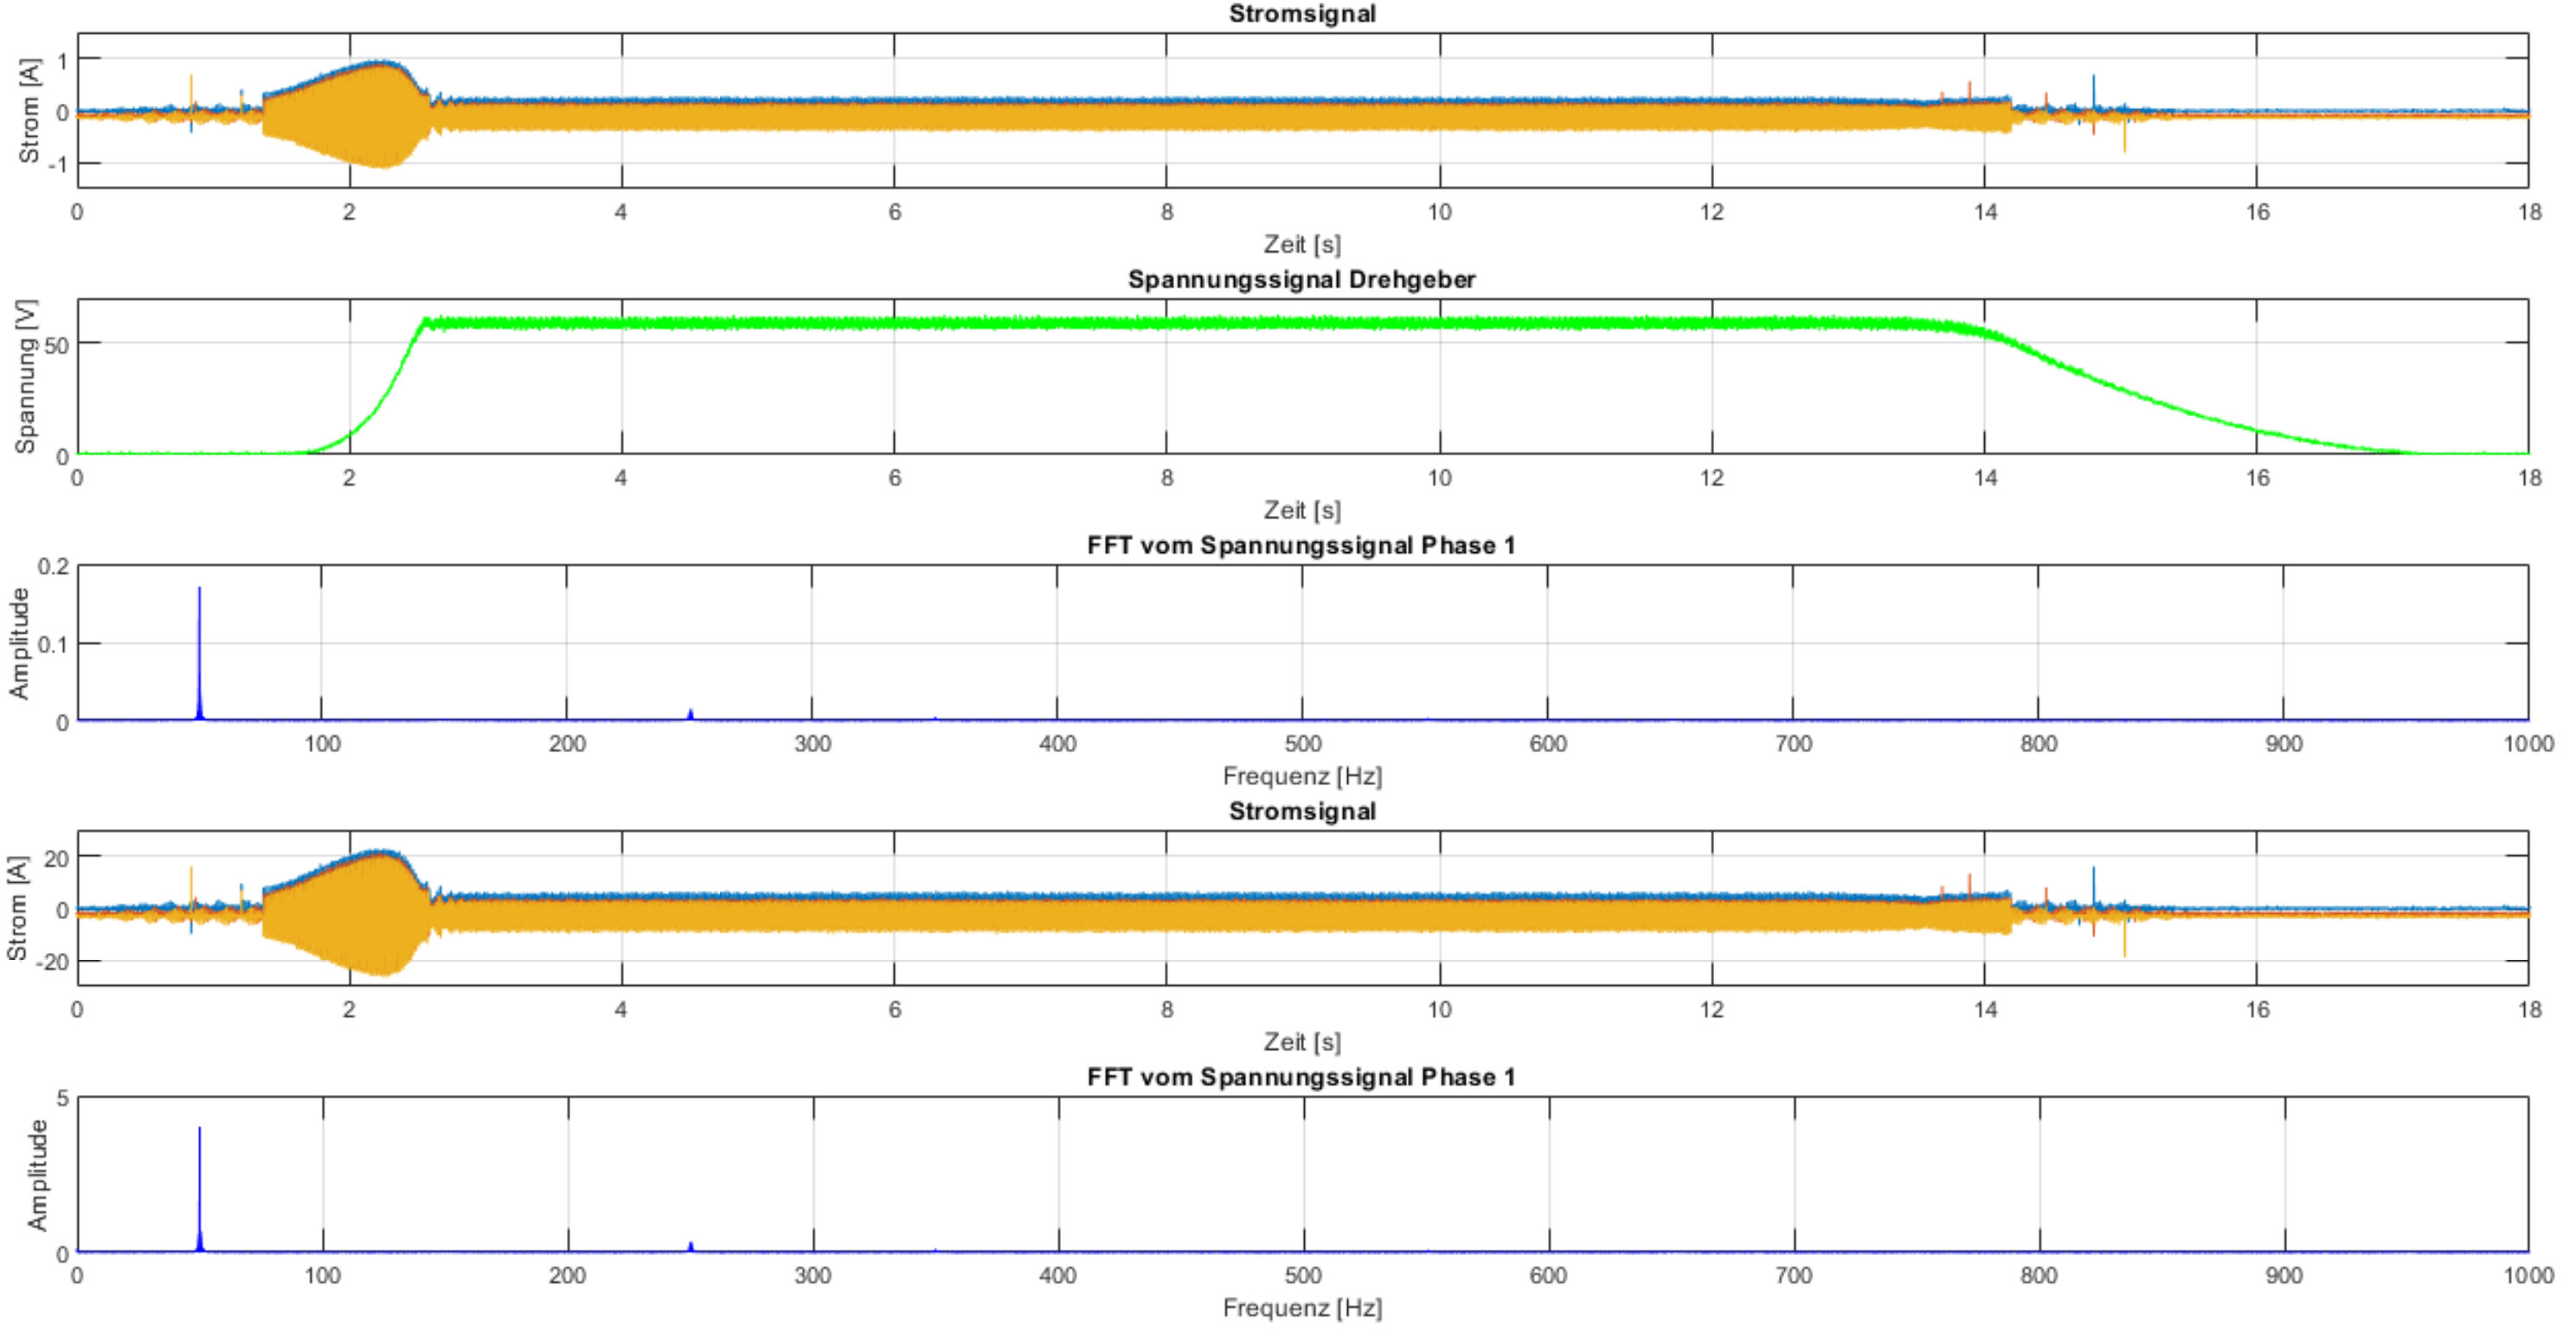
\includegraphics[width=\textwidth]{Messung_ASM_Sanft_langsam_stroeme.png}	
	\caption{Messung mit sanftem Auf- und Absteuern}\label{fig:Mess_Sanft_langsam_stroeme}
\end{figure}

Wie auch schon bei der Widerstandsmessung mit dem sanftem Auf- und Absteuern im Kapitel \ref{sec:Sanft_Widerstand_stroeme} beschrieben, sind auch bei der Messung mit der ASM die harmonische Oberschwingungen sehr klein. In der Tabelle \ref{tab:Sanft_langsam_ASM_stroeme} sind bei verschiedenen Frequenzen die Werte der Amplituden des FFTs aufgelistet. 

\begin{table}[ht!]
	\centering
	\begin{tabular}{|l|l|l|}
		\hline
		Frequenz {[}Hz{]} & Amplitude {[}A{]} & Verhältnis zur Grundschwingung	\\ \hline
		49.8              & 0.823             & 20.51\%							\\ \hline
		49.9              & 1.064             & 26.51\%							\\ \hline
		49.95             & 1.716             & 42.76\%							\\ \hline
		50                & 4.013             & 100\%							\\ \hline
		50.05             & 1.613             & 40.19\%							\\ \hline
		50.1              & 1.141             & 28.43\%							\\ \hline
		50.2              & 0.878             & 21.88\%							\\ \hline
		250               & 0.28              & 6.98\%							\\ \hline
	\end{tabular}
	\caption{Amplitudenwerte bei den harmonischen Oberschwingungen bei sanftem Auf- und Absteuern}\label{tab:Sanft_langsam_ASM_stroeme}
\end{table}

Die Peaks des Trägerbandes um \SI{50}{Hz} sind bis zu 40\%. Wie auch schon bei der Widerstandsmessung mit dem sanftem Auf- und Absteuern, sind diese Peaks sehr nahe an den \SI{50}{Hz}.


\newpage
\subsection{Messungen Spannungen}
Um die Werte des Laboraufbaues mit den Simulationen vergleichen zu können, wurden die Spannungen beim Widerstand und bei der ASM mit den verschiedenen Ansteuerungsarten gemessen. Dafür wurden die Spannungssignale als Grafik und als Tabelle mit den Werte des FFTs bei den harmonischen Oberwellen dargestellt. 

\subsubsection{Messungen Widerstand}
Für die Spannungsmessung beim Widerstand wurden die Schwingungspaketsteuerung mit einem Duty-cycle von 50\% und 80\%, das harte und sanfte Auf- und Absteuern. Die Messungen mit dem Phasenanschnitt von 60\textdegree \hspace{0.02cm} und 90\textdegree, welche die Normen im Kapitel \ref{sec:Stromnormen} nicht erfüllten, wurden bereits aussortiert und befinden sich im Anhang im Kapitel \ref{sec:Mess_Spannung_Widerstand}.


\subsubsection*{Schwingungspaket 50\%}
\begin{figure}[ht!]
	\centering
	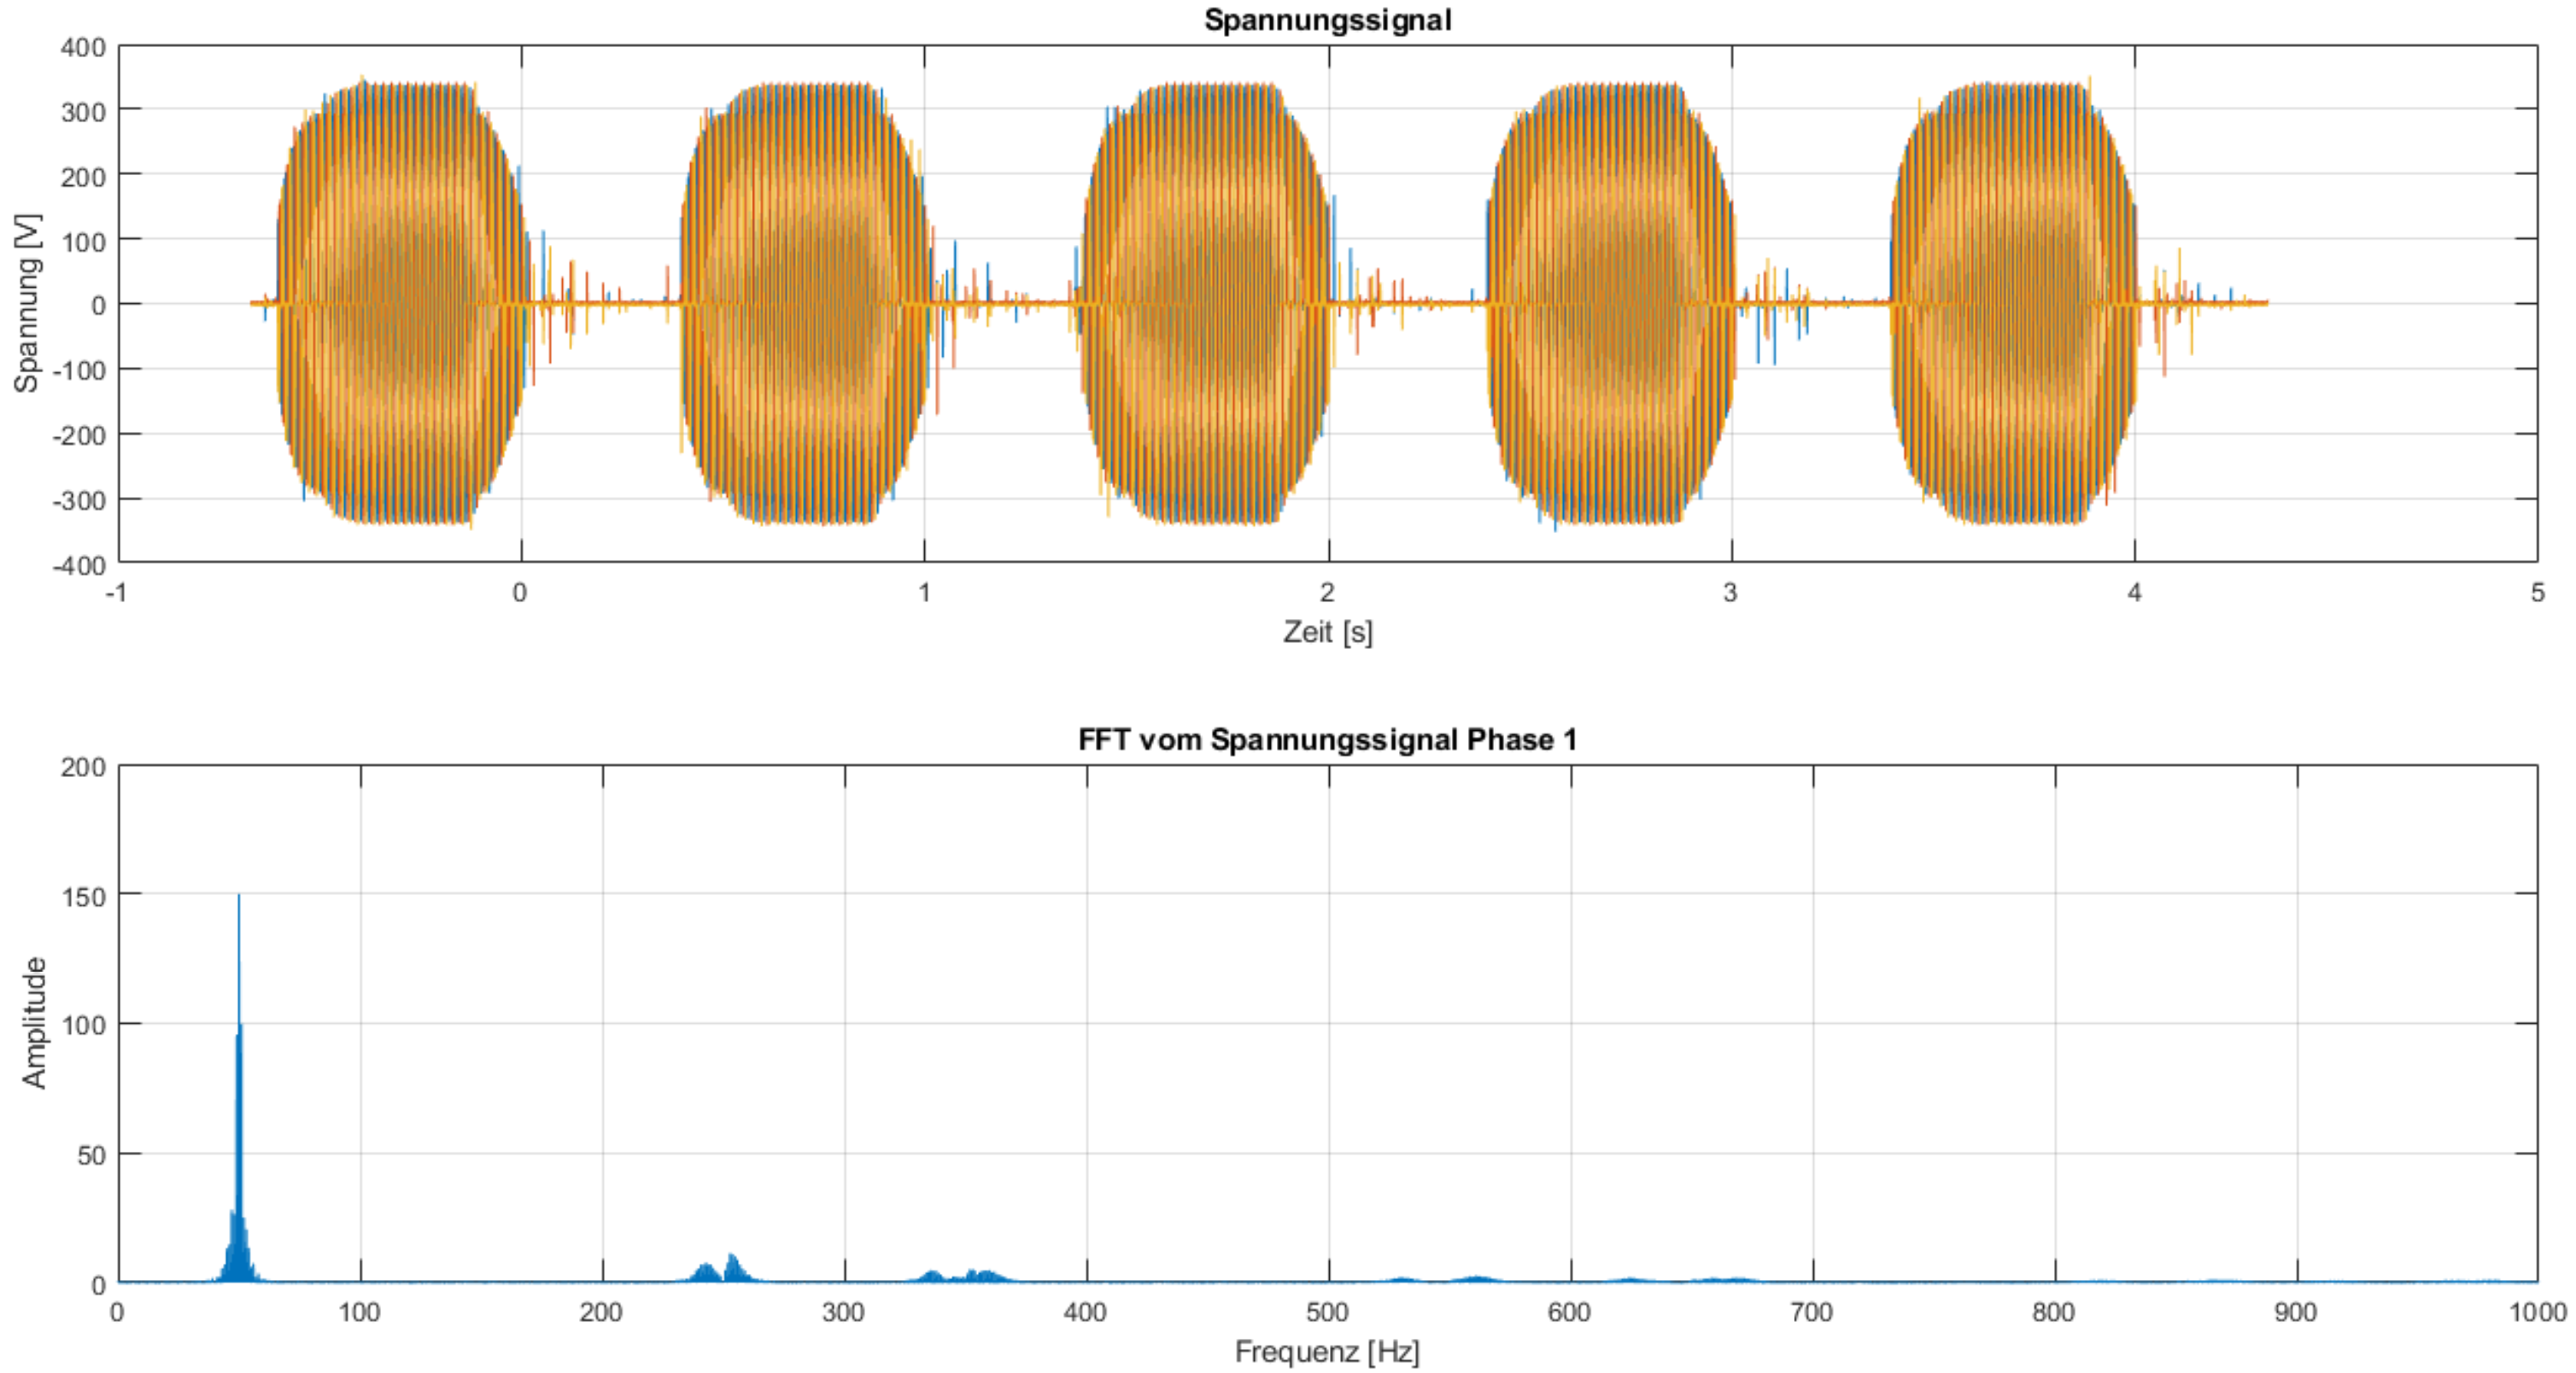
\includegraphics[width=\textwidth]{Messung_Widerstand_Schwing_0_5.png}	
	\caption{Messung mit Schwingungspaket 50\%}\label{fig:Mess_Schwing_50}
\end{figure}

Wie bei den Simulationen im Kapitel \ref{sec:Schwingungspaketsteuerung_Simulation} gezeigt, treten bei der Schwingungspaketsteuerung keine harmonische Oberwelle auf. Das FFT zeigt aber auch auf, dass das Trägerband bei der Grundschwingung relativ breit ist. Auf der Tabelle \ref{tab:Mess_Spannung_Schwing_50} sind die Werte der Amplituden der Sub- und Zwischenharmonischen aufgelistet. Dabei wurden die Werte aus dem FFT gelesen, welche sich bei der Grundschwingung befinden und eine hohe Amplitude besitzen. Zusätzlich wurde das Verhältnis zu Grundschwingung in Prozent angegeben, um die verschiedenen Verfahren vergleichen zu können.

\newpage
\begin{table}[ht!]
	\centering
	\begin{tabular}{|l|l|l|}
		\hline
		Frequenz {[}Hz{]} & Amplitude {[}V{]} & Verhältnis zur Grundschwingung \\ \hline
		46                & 14.7351           & 9.83\%                         \\ \hline
		47                & 28                & 18.68\%                        \\ \hline
		48                & 26.376            & 17.59\%                        \\ \hline
		49                & 95.6              & 63.77\%                        \\ \hline
		50                & 149.92            & 100\%                          \\ \hline
		51                & 99.8              & 66.57\%                        \\ \hline
		52                & 25.134            & 16.76\%                        \\ \hline
		53                & 20.6              & 13.74\%                        \\ \hline
	\end{tabular}
\caption{Amplitudenwerte bei der Frequenzen bei Schwingungspaket 50\%}\label{tab:Mess_Spannung_Schwing_50}
\end{table}

Es ist in der Tabelle ersichtlich, dass die beiden Frequenzen neben der Grundschwingung mehr als 60\% so hoch sind wie die Amplitude bei \SI{50}{Hz}. Selbst \SI{4}{Hz} neben der Grundschwingung beträgt das Verhältnis immer noch fast 10\%.\\

Die Werte der Tabelle \ref{tab:Mess_Spannung_Schwing_50} wurden mit denen des FFTs der Plecs-Simulation verglichen. Die Grafik und die Werten der Messung und der Simulation befinden sich im Kapitel \ref{sec:Vergleich_Mess_Sim_Schwing_50} im Anhang. Dabei wurde festgestellt, dass die Kurvenformen zwar ähnlich aussehen jedoch bei näherem betrachten gibt es grosse Unterschiede. In der Simulation schnellen nach dem Einschalten eines Paketes die Spannungen sogleich an ihren Spitzenwert wobei dies beim Laboraufbau nicht der Fall ist. 
Zwar wurde die Zeitdauer beim Laboraufbau gleich gewählt wie bei der Simulation aber war die Spannung nicht gleich lang auf dem Spitzenwert. Zusätzlich ist der Spitzenwert nicht bei beiden gleich hoch. Des weiteren sind alle Bauteile in der Simulation ideal wobei dies in der Praxis nicht der Fall ist. Die Standartabweichung aller aufgeführten Frequenzen beträgt: 7.912. Dieser Wert wurde mit Excel berechnet wobei die Frequenzen als Stichprobe angenommen wurden.



\newpage
\subsubsection*{Schwingungspaket 80\%}
\begin{figure}[ht!]
	\centering
	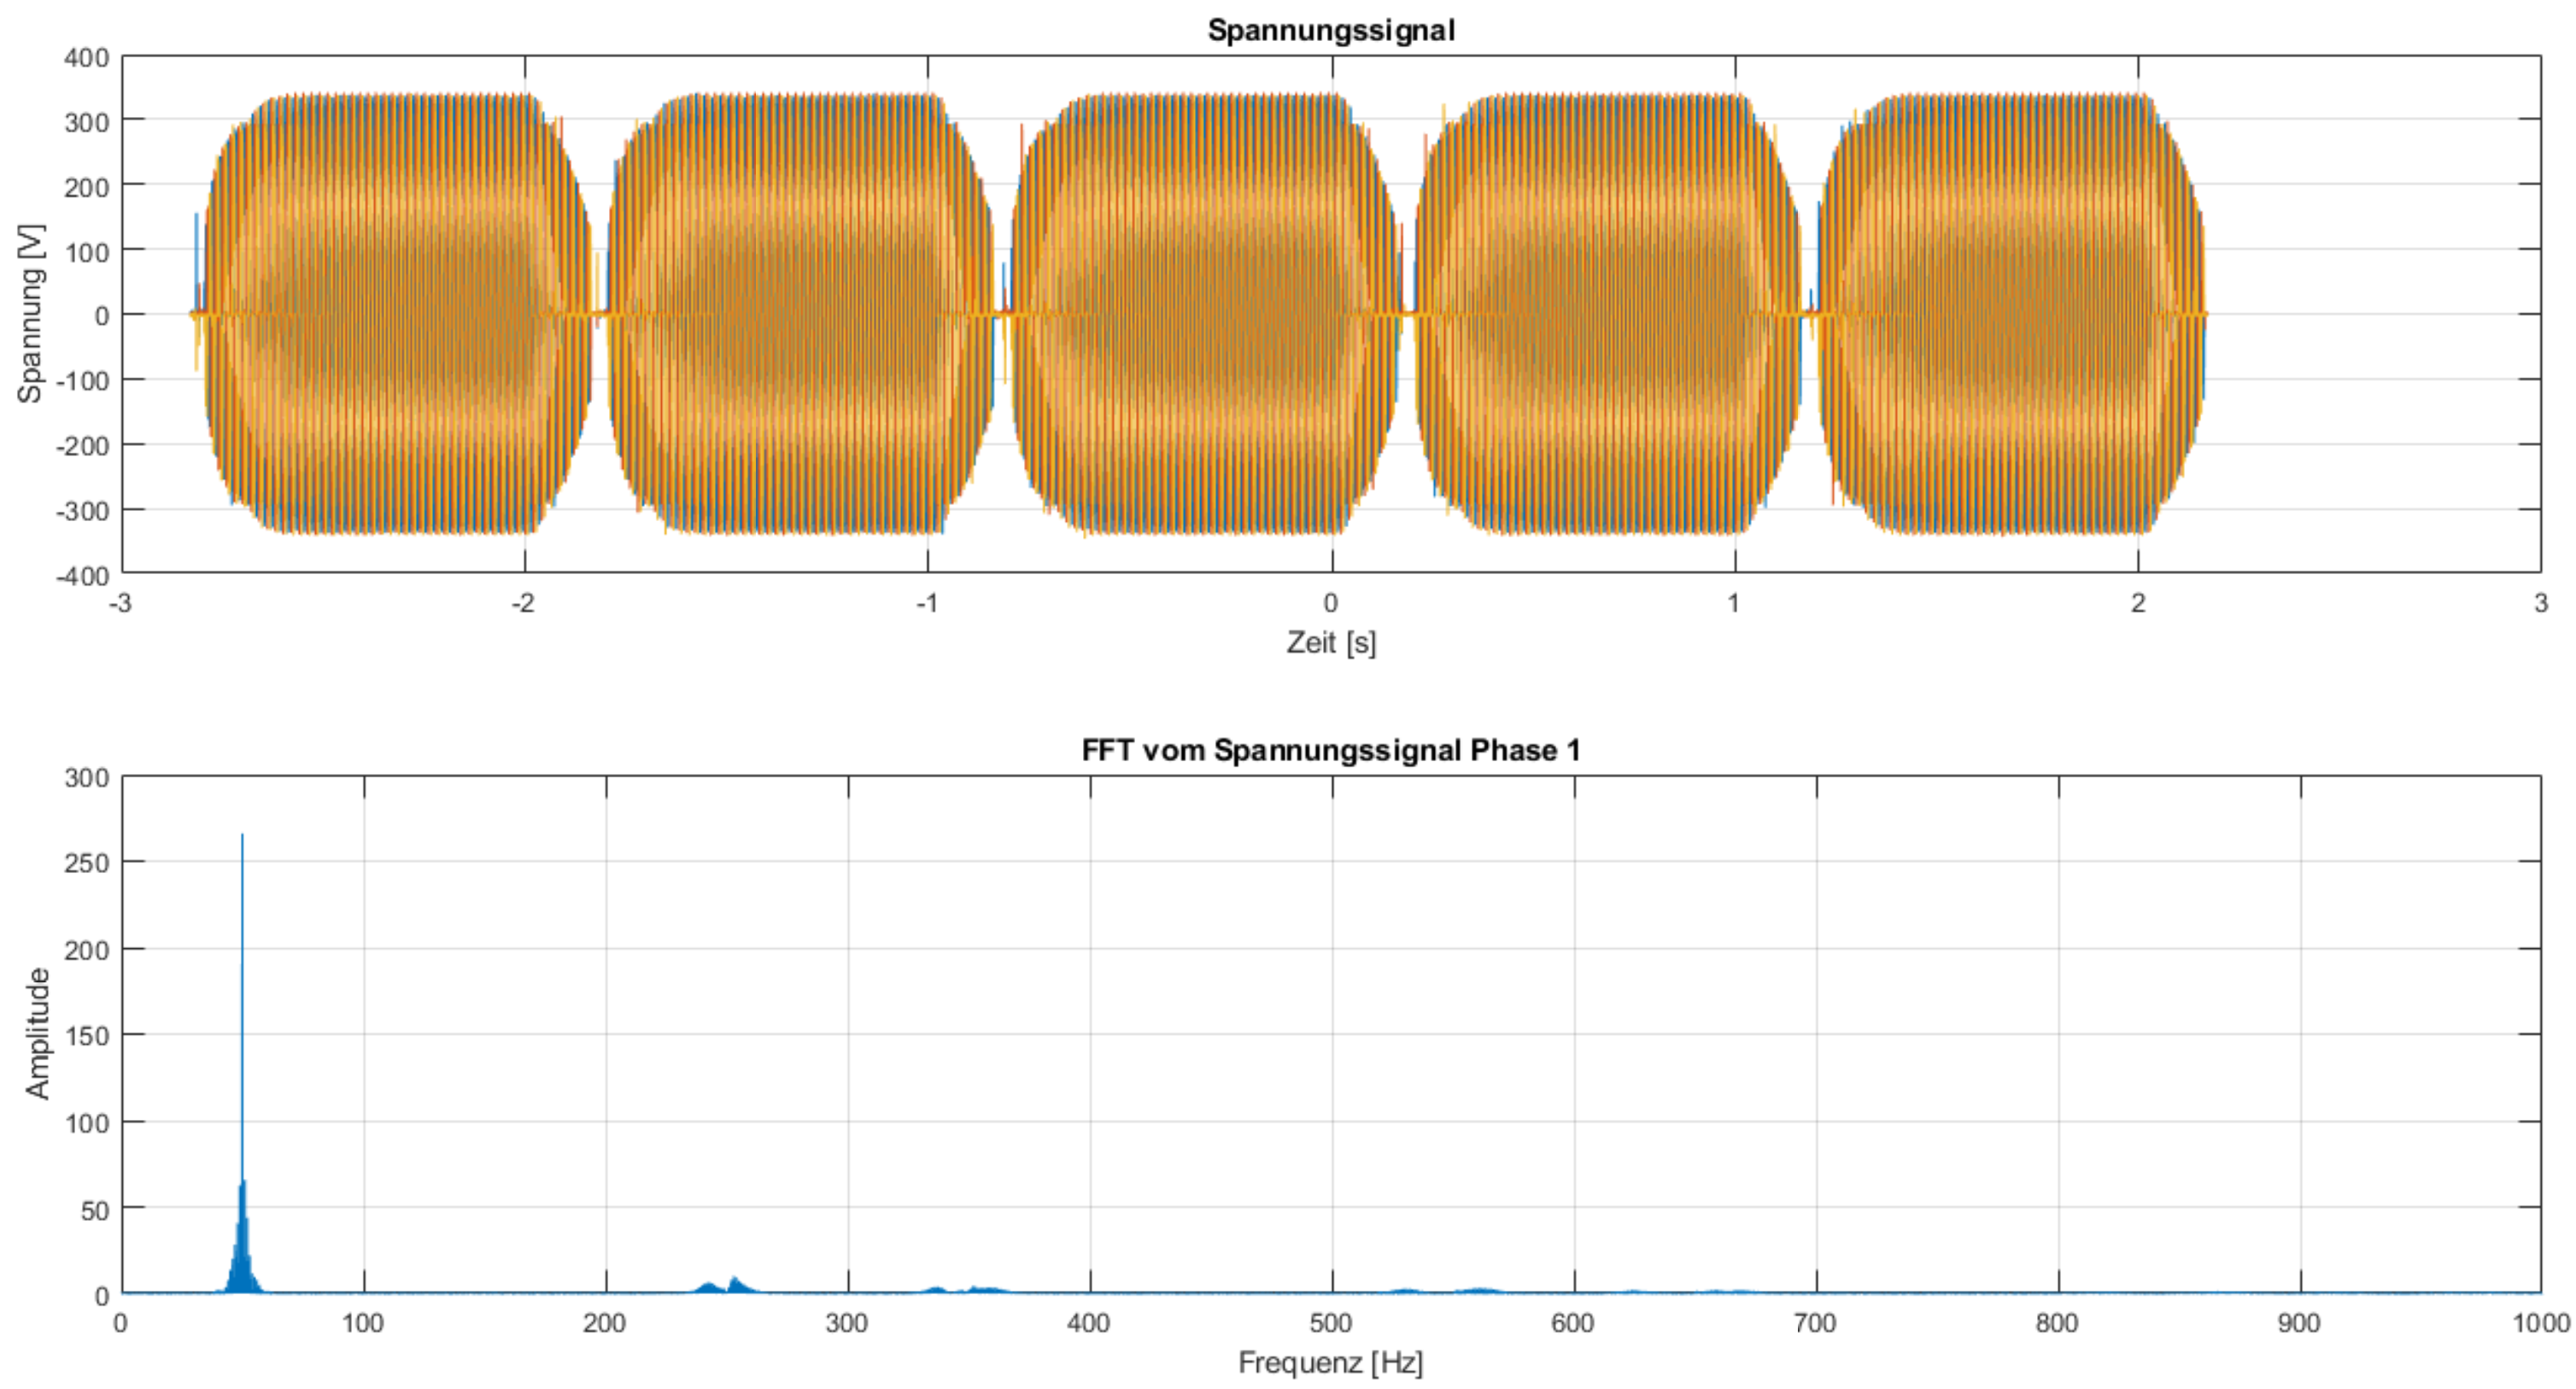
\includegraphics[width=\textwidth]{Messung_Widerstand_Schwing_0_8.png}	
	\caption{Messung mit Schwingungspaket 80\%}\label{fig:Mess_Schwing_80}
\end{figure}

Anders als beim Schwingungspaket mit 50\%, ist bei 80\% der Peak deutlich höher bei \SI{50}{Hz}. Da die volle Spannung im Verhältnis länger auf die volle Spannung geschaltet wird, ergibt dieses Sinn. In der Tabelle \ref{tab:Mess_Spannung_Schwing_80} befinden sich die Werte der Amplituden und deren Verhältnis zur Grundschwingung bei den gleichen Frequenzen wie bei der Schwingungspaketsteuerung 50\%.

\begin{table}[ht!]
	\centering
	\begin{tabular}{|l|l|l|}
		\hline
		Frequenz {[}Hz{]} & Amplitude {[}V{]} & Verhältnis zur Grundschwingung \\ \hline
		46                & 20.173            & 7.58\%                         \\ \hline
		47                & 28.26             & 10.62\%                        \\ \hline
		48                & 40.576            & 15.26\%                        \\ \hline
		49                & 62.694            & 23.57\%                        \\ \hline
		50                & 265.98            & 100\%                          \\ \hline
		51                & 65.7              & 24.7\%                         \\ \hline
		52                & 43.812            & 16.47\%                        \\ \hline
		53                & 21.939            & 8.25\%                         \\ \hline
	\end{tabular}
\caption{Amplitudenwerte bei der Frequenzen bei Schwingungspaket 80\%}\label{tab:Mess_Spannung_Schwing_80}
\end{table}

Wenn die Amplituden der Frequenzen \SI{49}{Hz} und \SI{51}{Hz} im Verhältnis zur Grundschwingung viel kleiner sind als bei der Schwingungspaketsteuerung mit 50\%. Die anderen aufgelisteten Frequenzen sind im Verhältnis zur Grundschwingung etwa gleich gross.\\


Wie bei der Schwingungspaketsteuerung mit 50\% wurden bei 80\% die Resultate der Messung und der Simulation verglichen. Die Tabelle mit den Werten und der grafische Vergleich befindet sich im Anhang in Kapitel \ref{sec:Vergleich_Mess_Sim_Schwing_80}. Auch hier gab es Abweichungen bei den verschiedenen Frequenzen zwischen der Simulation und der Messung. Diese waren aber bedeutend kleiner als bei dem Schwingungspaket mit 50\%, welches in einer kleineren Standartabweichung von 2.481 resultierte. Als Grund für die Abweichung gelten die gleichen Gründe, wie bei der Schwingungspaketsteuerung mit 50\%.



\newpage
\subsubsection*{Hartes Auf- und Absteuern}
\begin{figure}[ht!]
	\centering
	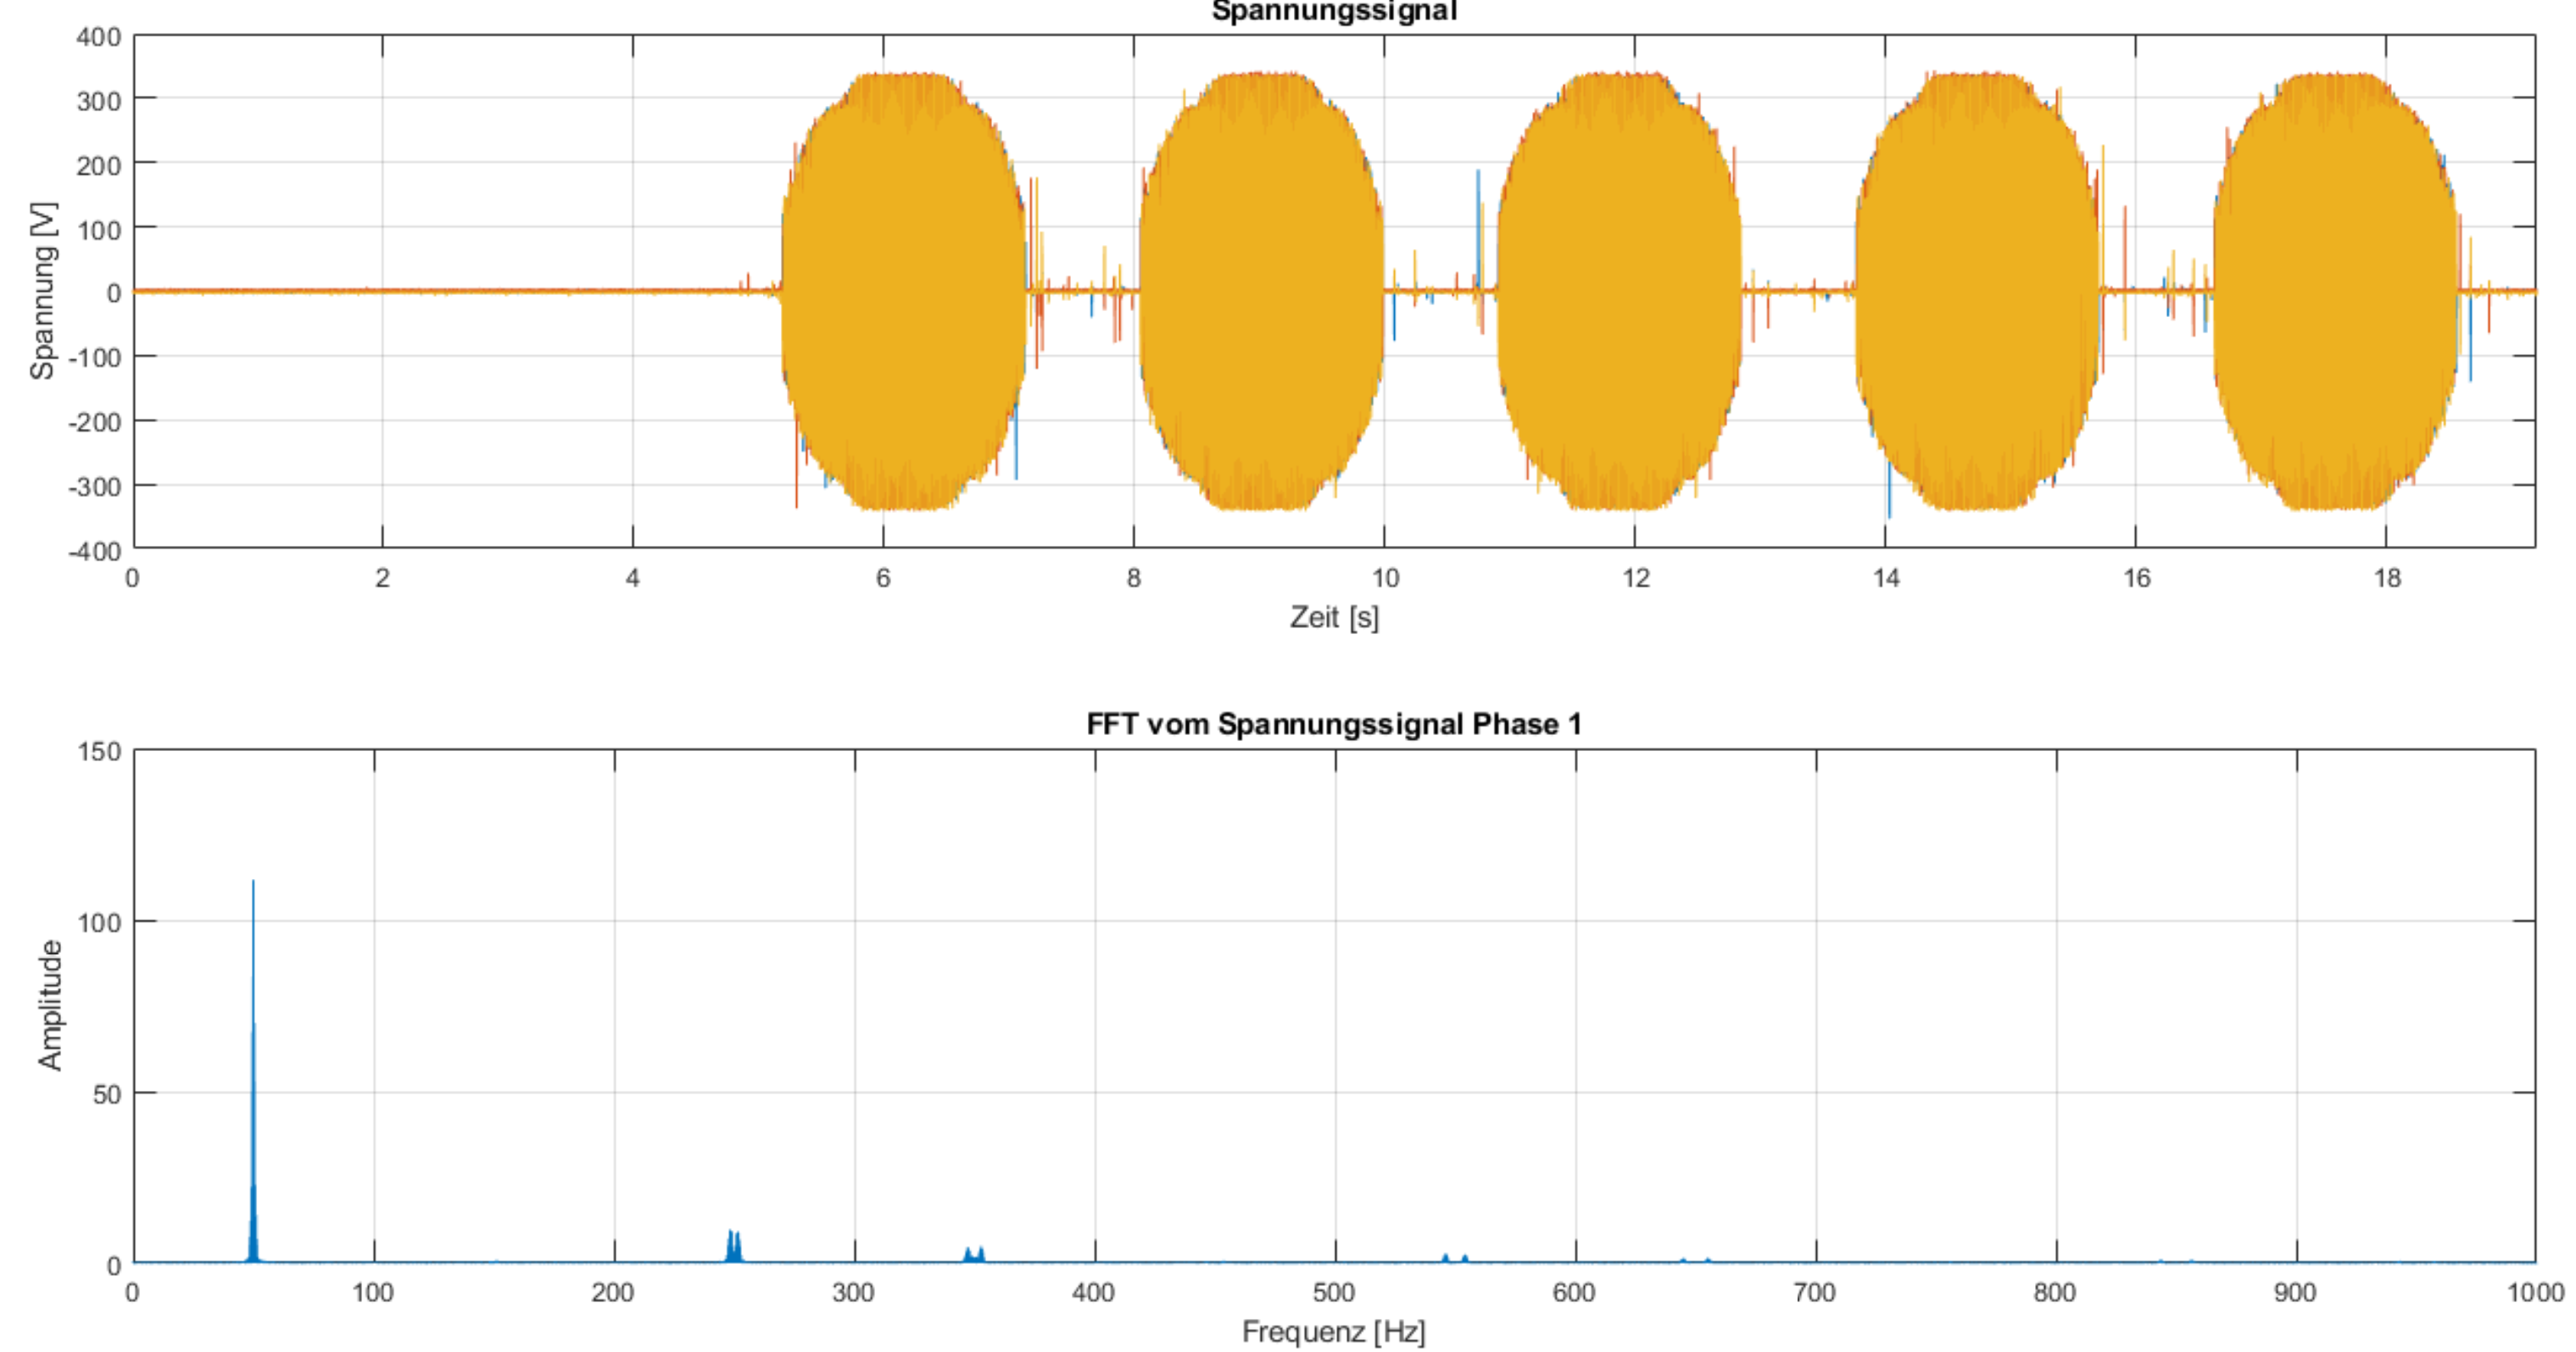
\includegraphics[width=\textwidth]{Mess_Widerstand_AufAb.png}	
	\caption{Messung mit Auf- und Absteuern}\label{fig:Mess_Sanft}
\end{figure}

Für die Tabelle \ref{tab:Mess_Spannung_AufAb_hart} wurden die höchsten Amplituden bei der Grundschwingung und bei der fünften Harmonische aufgelistet.

\begin{table}[ht!]
	\centering
	\begin{tabular}{|l|l|l|}
		\hline
		Frequenz {[}Hz{]} & Amplitude {[}V{]} & Verhältnis zur Grundschwingung \\ \hline
		49.65             & 67.126            & 60.11\%                        \\ \hline
		49.7              & 40.9583           & 36.68\%                        \\ \hline
		50                & 111.6763          & 100\%                          \\ \hline
		50.05             & 58.2021           & 52.12\%                        \\ \hline
		50.35             & 70.0651           & 62.74\%                        \\ \hline
		249               & 9.0297            & 8.09\%                         \\ \hline
		250               & 1.0487            & 0.94\%                         \\ \hline
		251 		      & 1.8206            & 1.63\%                         \\ \hline
	\end{tabular}
\caption{Amplitudenwerte bei der Frequenzen bei hartes Auf- und Absteuern}\label{tab:Mess_Spannung_AufAb_hart}
\end{table}

Wie auch bei den Schwingungspaketsteuerungen, tritt bei dem harten Auf- und Absteuern die harmonischen Oberschwingung praktisch nicht mehr auf. Die fünfte Harmonische besitzt nur ein Verhältnis von unter einem Prozent der Grundschwingung. Jedoch treten auch hier wieder die Sub- und Zwischenharmonische auf. Diese betragen bei den Frequenzen \SI{49.65}{Hz} und \SI{50.35}{Hz} über 60\%. \\
Für den Vergleich mit dem harten Auf- und Absteuern gibt es einen Unterschied der Signaldauern. Während bei der Simulation das Auffahren \SI{0.2}{s} dauert, benötigt der Laboraufbau mit fast \SI{0.8}{s} deutlich länger. Ein weiterer Unterschied waren bei der Messung die Zeitdauer zwischen den verschiedenen Auf- und Absteuerpakete. Da der Thyristorsteller nicht sehr schnell reagiert, dauerte es fast \SI{1}{s} bis das nächste Paket anfangen konnte. Diese Gründe erklären den grossen Unterschied zwischem dem FFT der Simulation und der Messung. Berechnet wurde eine Standartabweichung von 19.812 wobei dieser Wert 2.5 mal gross ist, wie die Standartabweichung des Schwingungspaketes mit 50\%.



\newpage
\subsubsection*{Sanftes Auf- und Absteuern}
\begin{figure}[ht!]
	\centering
	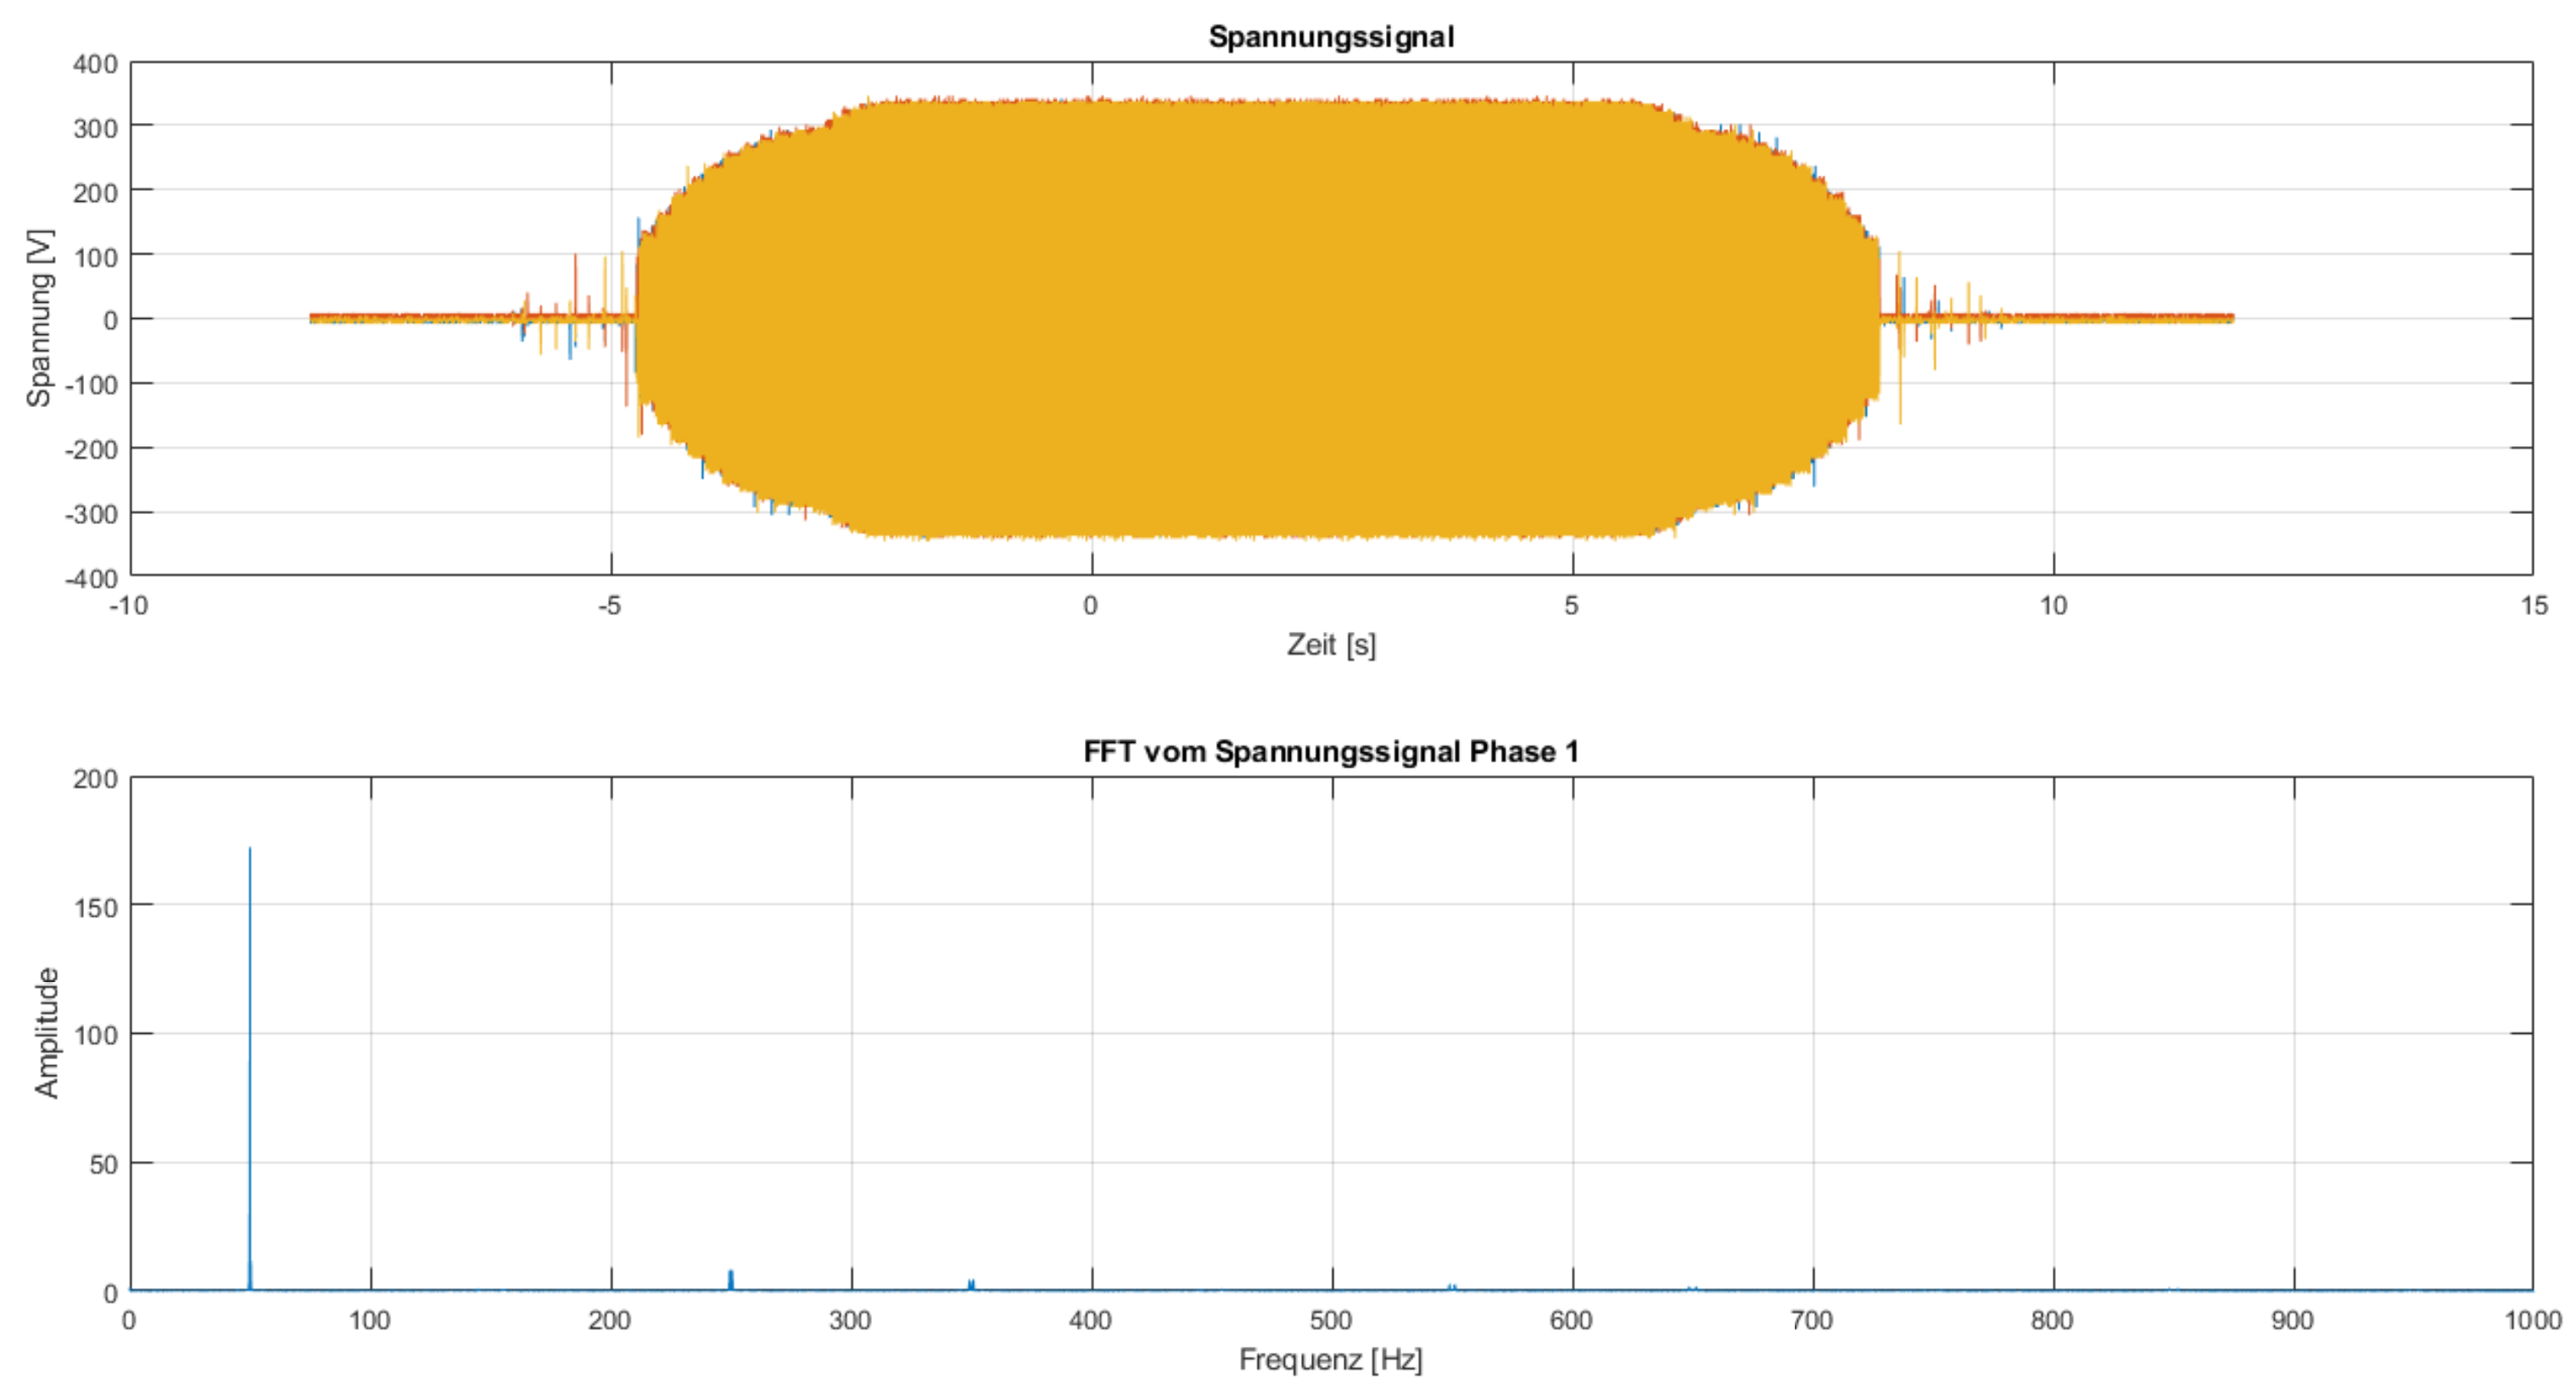
\includegraphics[width=\textwidth]{Messung_Widerstand_Sanft_langsam.png}	
	\caption{Messung mit sanftem Auf- und Absteuern}\label{fig:Mess_Sanft_langsam}
\end{figure}

Im visuellen Vergleich zum hartem Auf- und Abfahren zeigt das FFT auf, das die Frequenzbänder dünner sind und das der Peak bei \SI{50}{Hz} grösser ist. Es wurden in der Tabelle \ref{tab:Mess_Spannung_AufAb_sanft} wieder die höchsten Amplituden der Frequenzen um die Grundschwingung und der fünften Harmonischen aufgezeigt. \todo{Einfügen Vergleich Simulation}

\begin{table}[ht!]
	\centering
	\begin{tabular}{|l|l|l|}
		\hline
		Frequenz {[}Hz{]} & Amplitude {[}V{]} & Verhältnis zur Grundschwingung \\ \hline
		49.8              & 18.522            & 10.75\%                        \\ \hline
		49.85             & 26.576            & 15.43\%                        \\ \hline
		49.9              & 29.507            & 17.131\%                       \\ \hline
		49.95             & 91.266            & 52.99\%                        \\ \hline
		50                & 172.241           & 100\%                          \\ \hline
		50.05             & 116.719           & 67.76\%                        \\ \hline
		50.1              & 28.629            & 16.62\%                        \\ \hline
		50.15             & 30.076            & 17.46\%                        \\ \hline
		50.2              & 18.72             & 10.87\%                        \\ \hline
		249.6             & 8.183             & 4.75\%                         \\ \hline
		250               & 1.158             & 0.67\%                         \\ \hline
		250.4             & 7.466             & 4.33\%                         \\ \hline
	\end{tabular}
\caption{Amplitudenwerte bei der Frequenzen bei Sanftes Auf- und Absteuern}\label{tab:Mess_Spannung_AufAb_sanft}
\end{table}

Der Vergleich mit der Tabelle \ref{tab:Mess_Spannung_AufAb_hart} zeigt auf, dass die höchsten Peaks bei den Sub- und Zwischenharmonischen nicht mehr bei den Frequenzen \SI{49.65}{Hz} und \SI{50.35}{Hz} liegen, sonder näher bei der Grundschwingung liegen, bei \SI{49.95}{Hz} und \SI{50.05}{Hz}. Das Verhältnis bei \SI{250}{Hz} zur Grundschwingung ist beim sanftem Auf- und Abfahren kleiner geworden als beim harten Auf- und Abfahren. Aber wie auch bei \SI{50}{Hz} sind die höchsten Amplituden näher an der harmonische Schwingung. \\
Der Vergleich mit der Simulation und der Messung für den sanften Auf- und Abfahren, welches sich im Kapitel \ref{sec:Vergleich_Mess_Sim_sanft_AufAb} im Anhang befindet, zeigt grosse Unterschiede bei den Amplituden auf. Ein grosser Grund dafür ist, dass bei der Simulation das Hoch- und Runterfahren eine Zeitdauer von \SI{0.3}{s} haben, wobei für die Messung diese Zeitdauer \SI{3}{s} beträgt. Zusätzlich ist bei der Simulation während \SI{6}{s} die Spannung auf dem Spitzenwert, beim Laboraufbau sind es eher \SI{7}{s}.  Berechnet wurde für die Standartabweichung ein Wert von 88.904. Diese Standartabweichung sagt aus, dass die beiden Funktionen überhaupt nicht miteinander verglichen werden können, da die Abweichung sehr gross ist.






\subsubsection{Messungen ASM}
Um zu analysieren, wie sich der Thyristorsteller bei einer ohmsch-induktiver Last verhält, wurden die Messungen mit einer ASM gemacht. Auch hier wurden die verschiedenen Ansteuerungsarten, Phasenanschnitt mit 60\textdegree \hspace{0.02cm} und 90\textdegree \hspace{0.02cm}, Schwingungspaket mit 50\% und 80\%, und dem harte und sanfte Auf- und Absteuern. Dabei wurde festgestellt, dass die Schwingungspaketsteuerung und das harte Auf- und Absteuern sich nicht für eine ASM eignen. \todo{Begründen wieso nicht}
Deswegen wurde diese im Anhang im Kapitel \todo{Kapitel ASM Messungen Spannung} eingefügt. 

\subsubsection*{Phasenanschnitt 60\textdegree}
\begin{figure}[ht!]
	\centering
	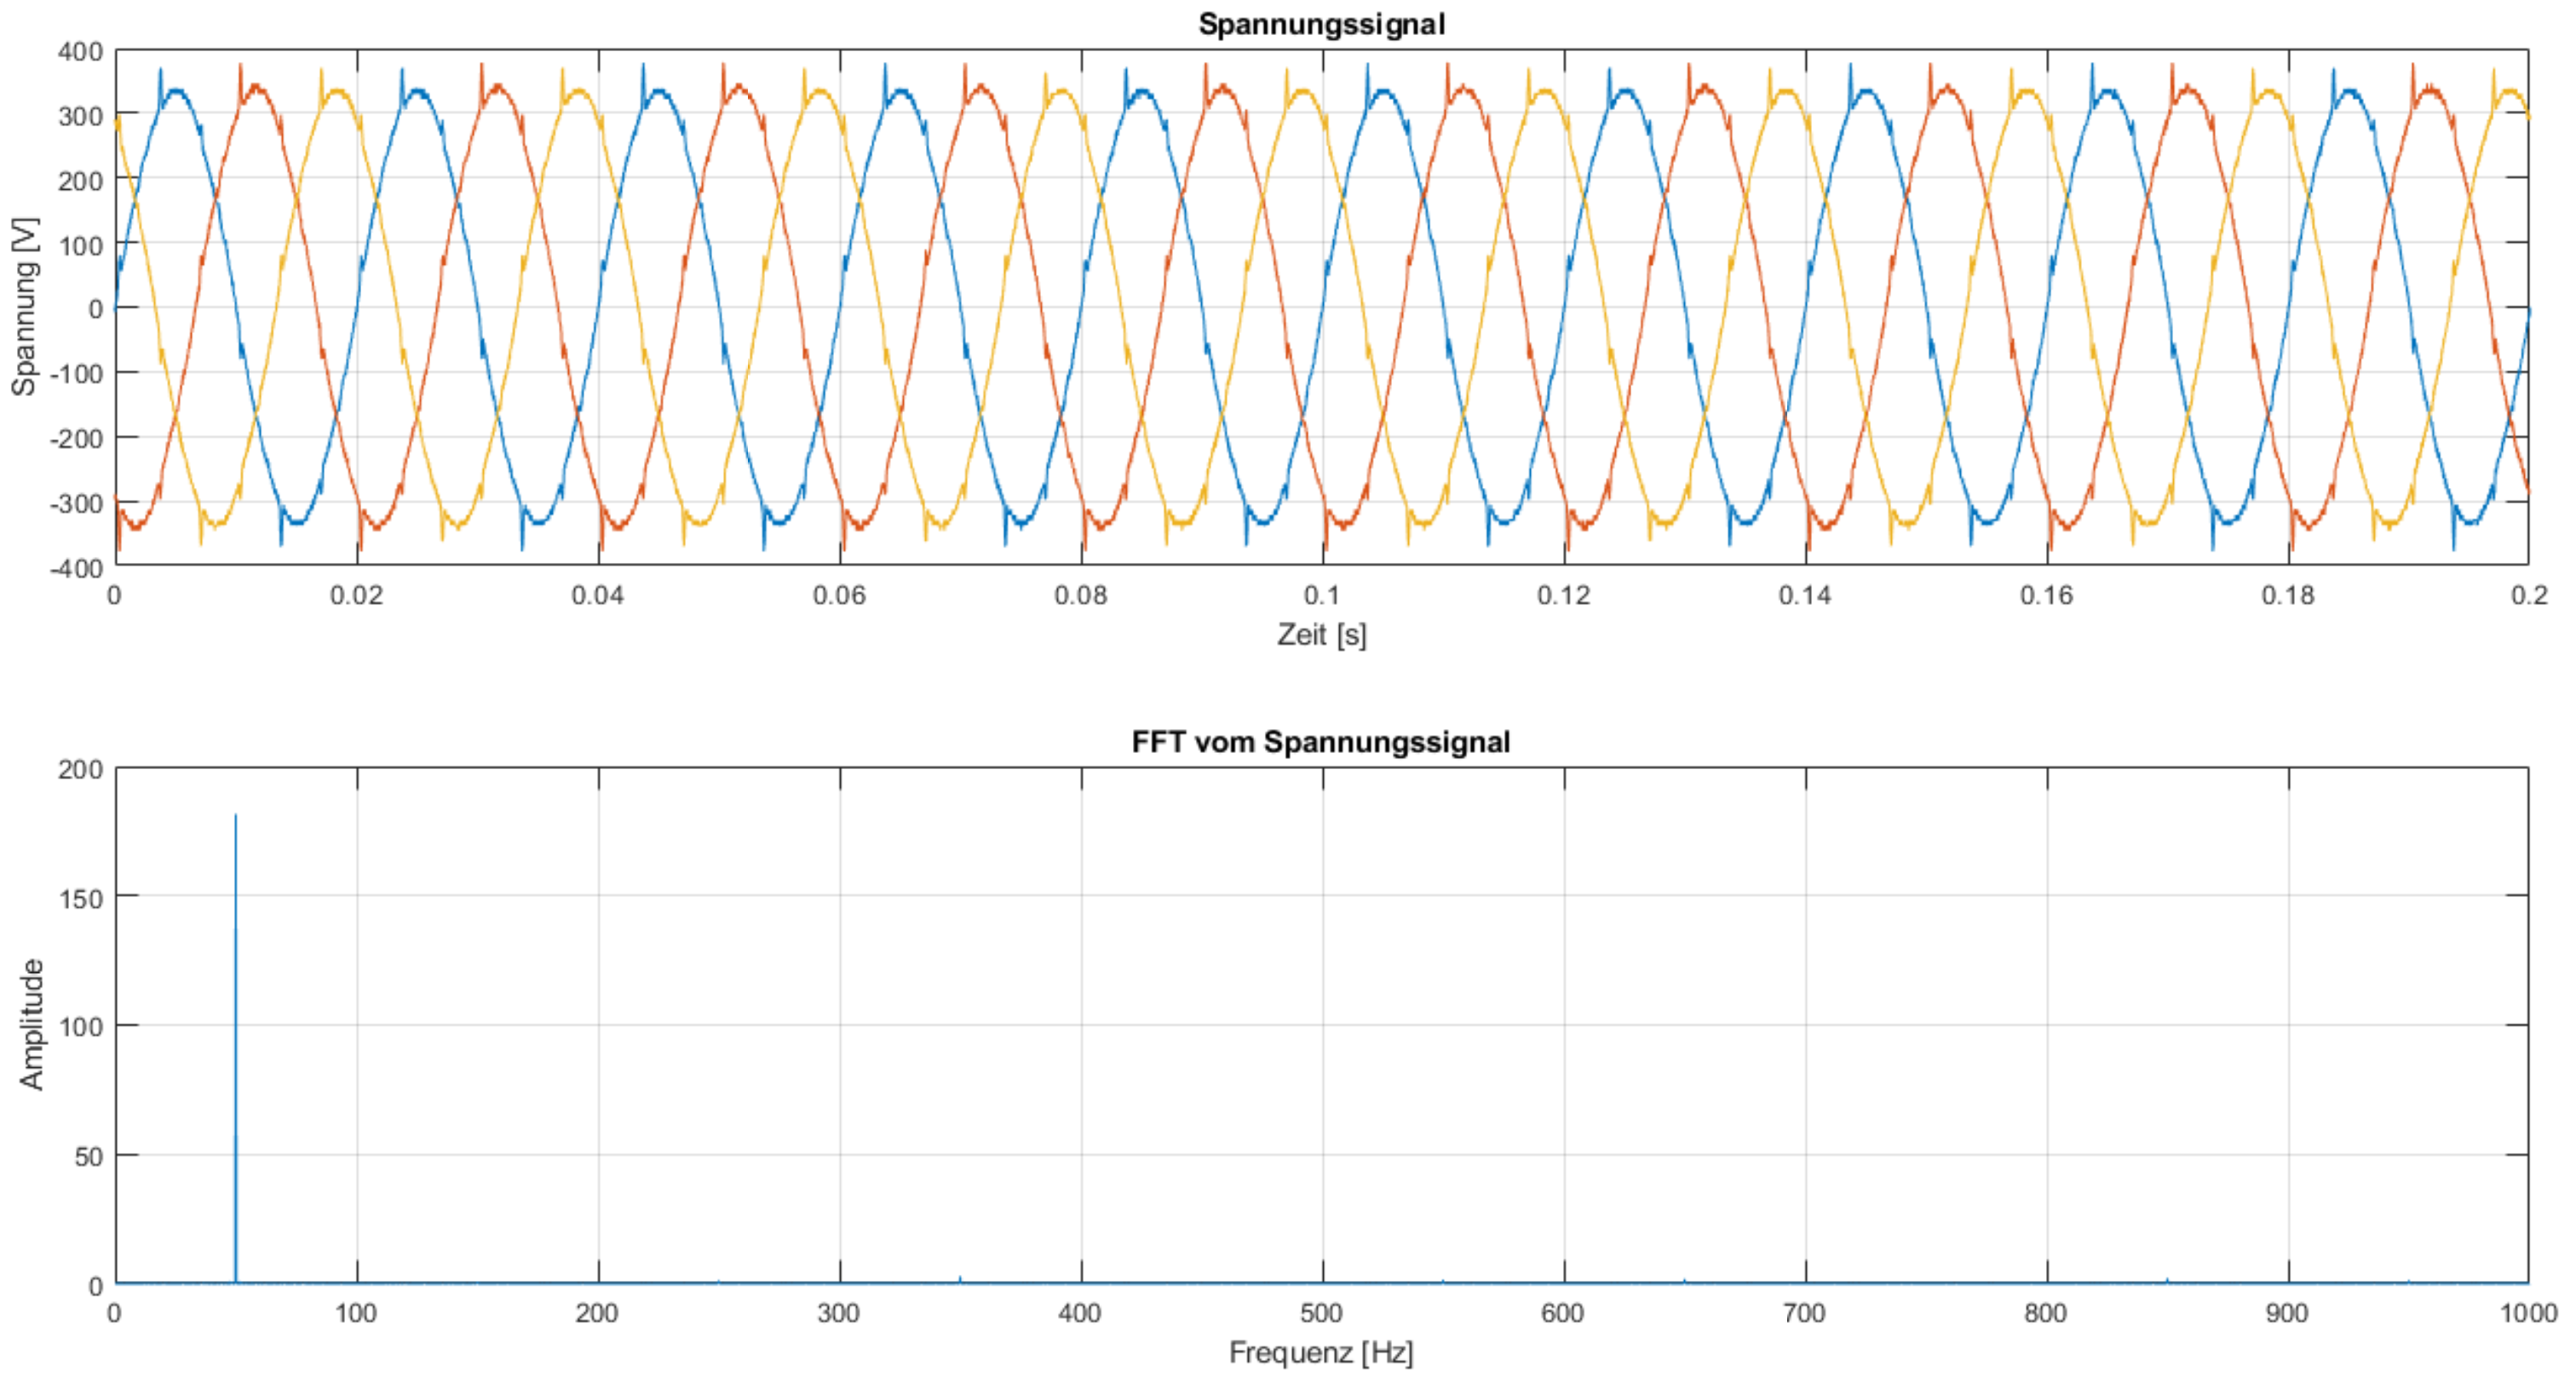
\includegraphics[width=\textwidth]{Messung_ASM_Phas_60grad.png}	
	\caption{Messung mit Phasenanschnitt 60\textdegree}\label{fig:Mess_ASM_Phas60}
\end{figure}

Beim Ansteuern mit dem Winkel von 60\textdegree \hspace{0.02cm} wurde bemerkt, dass die Maschine bereits mit maximaler Drehzahl dreht. Es macht bei den Spannungssignalen keinen Unterschied ob die ASM mit einem Winkel von 60\textdegree \hspace{0.02cm} oder 0\textdegree \hspace{0.02cm} angesteuert wird.
Anders als beim Phasenanschnitt mit 60\textdegree\hspace{0.02cm} bei ohmschen Lasten, treten bei ohmsch-induktiven Lasten fast keine harmonischen Oberschwingungen. Da diese Peaks nicht im FFT ersichtlich sind, wurden die Amplituden der Oberschwingungen bis zur elften Ordnung auf der Tabelle \ref{tab:Mess_Spannung_ASM_Phas60} aufgeführt. 
\newpage
\begin{table}[ht!]
	\centering
	\begin{tabular}{|l|l|l|}
		\hline
		Oberschwingungsordnung & Amplitude {[}V{]} & Verhältnis zur Grundschwingung \\ \hline
		1                      & 181.5519          & 100\%                          \\ \hline
		5                      & 1.1065            & 0.61\%                         \\ \hline
		7                      & 2.8728            & 1.58\%                         \\ \hline
		11                     & 1.4537            & 0.8\%                          \\ \hline
	\end{tabular}
\caption{Amplitudenwerte bei der Frequenzen bei Phasenanschnitt 60\textdegree}\label{tab:Mess_Spannung_ASM_Phas60}
\end{table}

Im Verhältnis zur Grundschwingung betragen die Amplituden der harmonischen Oberwellen maximal 1.58\% bei der siebten Ordnung. 

\newpage
\subsubsection*{Phasenanschnitt 90\textdegree}
\begin{figure}[ht!]
	\centering
	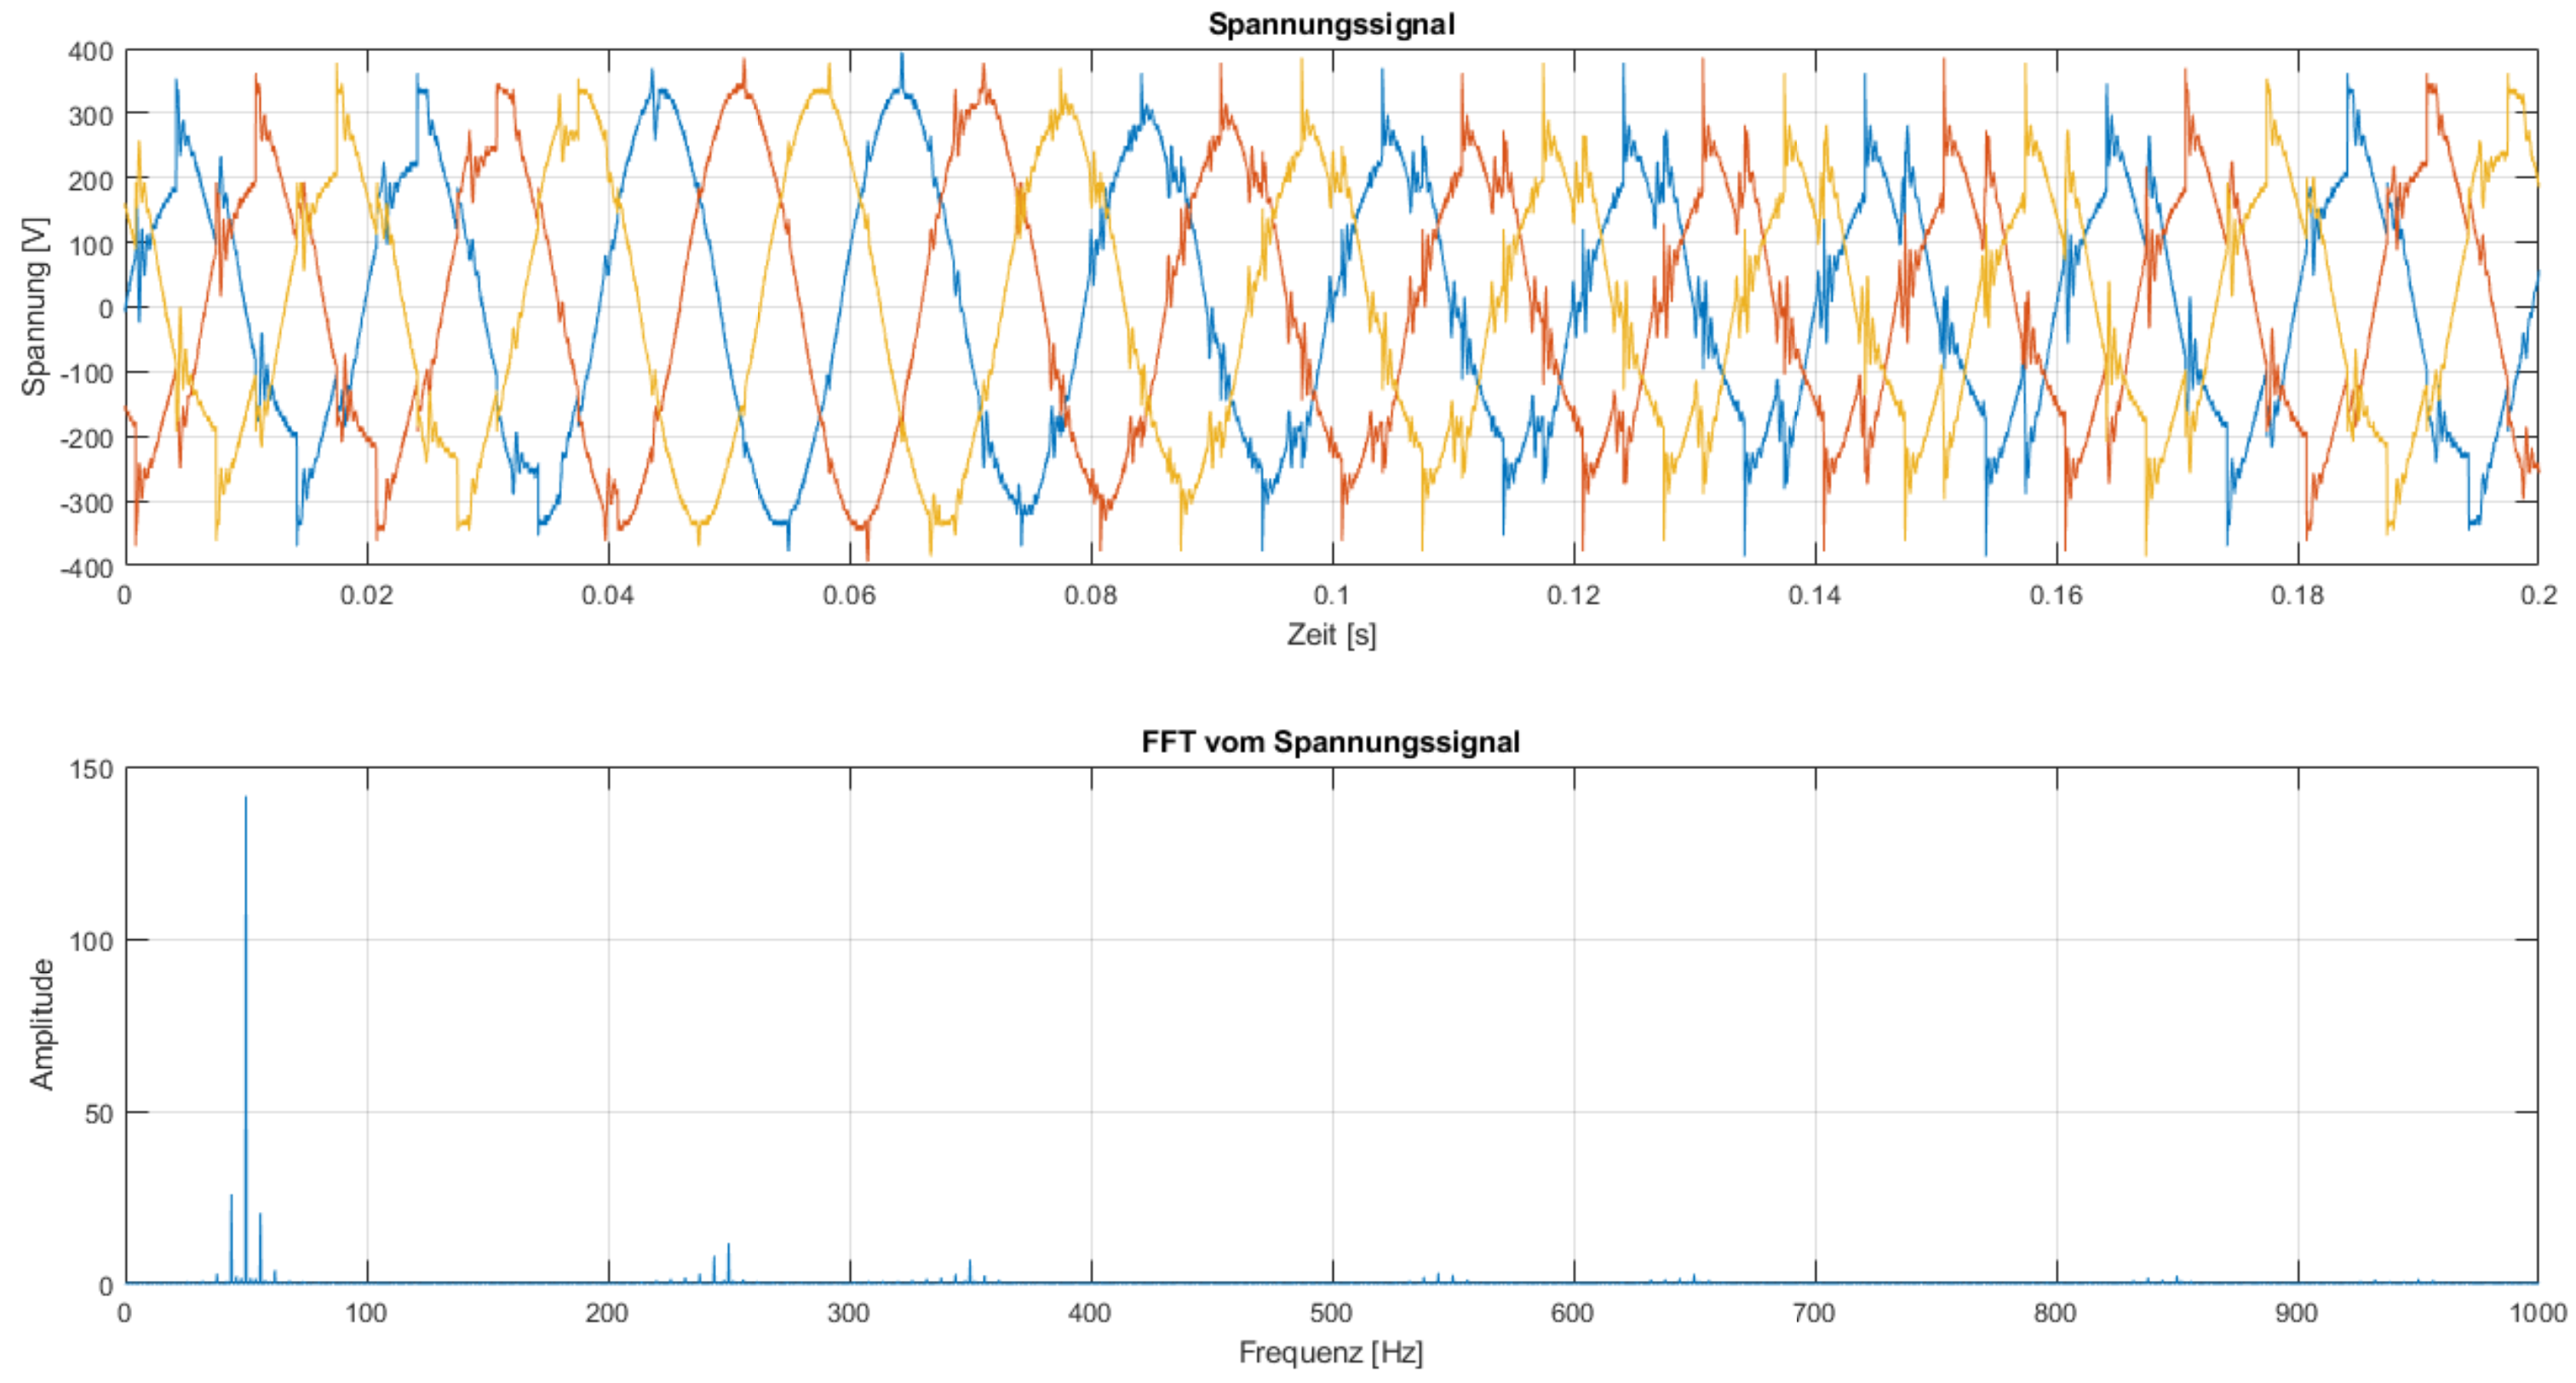
\includegraphics[width=\textwidth]{Messung_ASM_Phas_90grad.png}	
	\caption{Messung mit Phasenanschnitt 90\textdegree}\label{fig:Mess_ASM_Phas90}
\end{figure}

Anders als beim Phasenanschnitt mit 60\textdegree, beginnt dies ASM bei einem Winkel von 90\textdegree \hspace{0.02cm} zu schwingen. Dieses Schwingen ist gut ersichtlich in der Abbildung \ref{fig:Mess_ASM_Phas90} beim Spannungsverlauf. Dieses verhält sich nicht wie bei einem Phasenanschnitt erwartet konstant. Auch existieren grosse Unterschiede beim FFT mit dem Phasenanschnitt 60\textdegree \hspace{0.02cm} auf der Abbildung \ref{fig:Mess_ASM_Phas60}. Zum einen treten bei 00\textdegree \hspace{0.02cm} Sub- und Zwischenharmonische auf, sowie harmonische Oberwellen. Die Amplituden und das Verhältnis zur Grundschwingung sind für die erste, fünfte und siebte Harmonische, sowie deren Trägerbänder in der Tabelle \ref{tab:Mess_Spannung_ASM_Phas90} aufgelistet. 
\newpage
\begin{table}[ht!]
	\centering
	\begin{tabular}{|l|l|l|}
		\hline
		Frequenz {[}Hz{]} & Amplitude {[}V{]} & Verhältnis zur Grundschwingung \\ \hline
		44                & 25.896            & 18.31\%                        \\ \hline
		50                & 141.3976          & 100\%                          \\ \hline
		56                & 20.4508           & 14.46\%                        \\ \hline
		244               & 7.9778            & 5.64\%                         \\ \hline
		250               & 11.6537           & 8.24\%                         \\ \hline
		256               & 1.1655            & 0.82\%                         \\ \hline
		344               & 2.7272            & 1.93\%                         \\ \hline
		350               & 6.8988            & 4.88\%                         \\ \hline
		356               & 2.3509            & 1.66\%                         \\ \hline
	\end{tabular}
\caption{Amplitudenwerte bei der Frequenzen bei Phasenanschnitt 90\textdegree}\label{tab:Mess_Spannung_ASM_Phas90}
\end{table}

Es ist ersichtlich, dass das Verhältnis zur Grundschwingung bei den Harmonische viel grösser ist als beim Phasenanschnitt mit einem Winkel von 60\textdegree. 

\newpage
\subsubsection*{Sanftes Auf- und Absteuern}
\begin{figure}[ht!]
	\centering
	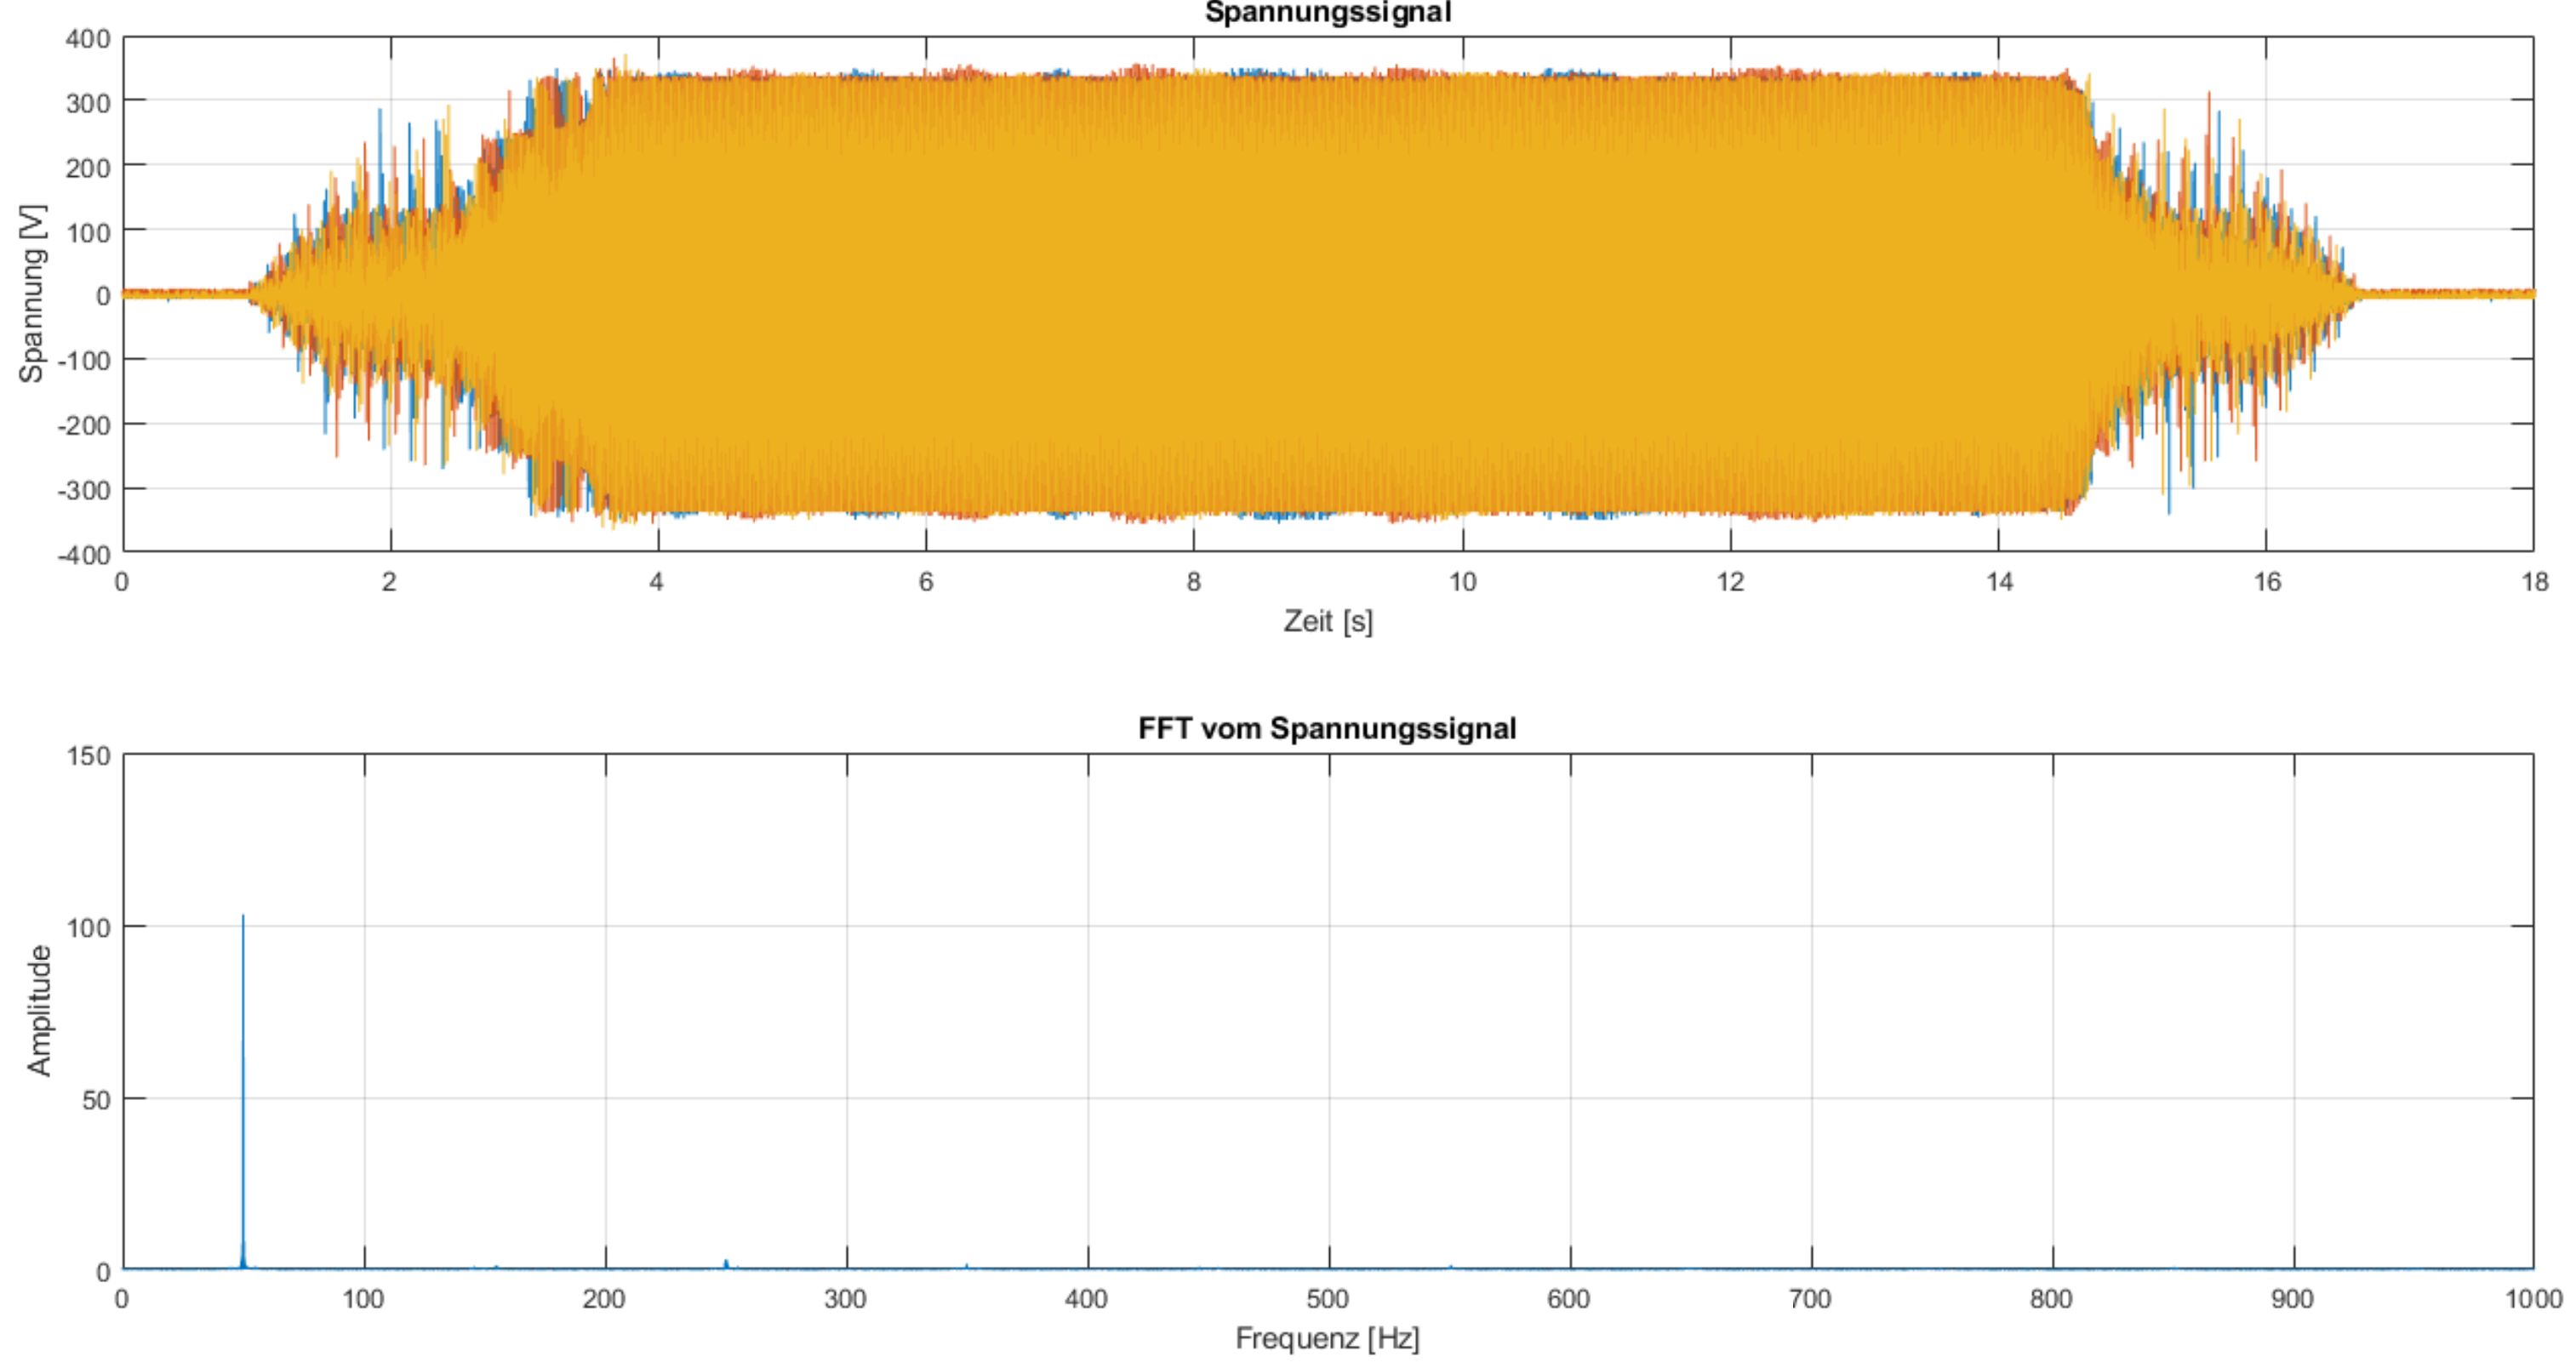
\includegraphics[width=\textwidth]{Messung_ASM_Sanft_langsam.png}	
	\caption{Messung mit sanftem Auf- und Absteuern}\label{fig:Mess_ASM_Sanft_langsam}
\end{figure}

Die Resultate der FFT-Berechnungen befinden sich in der Tabelle \ref{tab:Mess_Spannung_ASM_AufAb_sanft}. \todo{Mehr hinschrieben}


\begin{table}[ht!]
	\centering
	\begin{tabular}{|l|l|l|}
		\hline
		Frequenz {[}Hz{]} & Amplitude {[}V{]} & Verhältnis zur Grundschwingung \\ \hline
		49.85             & 17.3653           & 16.85\%                        \\ \hline
		49.95             & 70.316            & 68.23\%                        \\ \hline
		50                & 103.0639          & 100\%                          \\ \hline
		50.05             & 40.167            & 38.97\%                        \\ \hline
		50.1              & 20.209            & 19.61\%                        \\ \hline
		249.95            & 2.607             & 2.53\%                         \\ \hline
		250               & 1.689             & 1.64\%                         \\ \hline
		250.05            & 2.5084            & 2.43\%                         \\ \hline
	\end{tabular}
\caption{Amplitudenwerte bei der Frequenzen bei sanftem Auf- und Absteuern}\label{tab:Mess_Spannung_ASM_AufAb_sanft}
\end{table}

Beim sanftem Auf- und Abfahren treten Harmonische Oberwellen auf, diese sind im Verhältnis zur Grundschwingung jedoch unter zwei Prozent. Wie auch bei dem sanftem Auf- und Abfahren beim Widerstand sind die höchsten Amplituden des Trägerbandes der Grundschwingung bei \SI{49.95}{Hz} und \SI{50.05}{Hz}, also sehr nahe bei \SI{50}{Hz}.

\newpage
\subsection{Sparvariante}
Wie im Kapitel \ref{Spar-Ansteuerung} beschrieben, werden bei der Sparvariante nur ein oder zwei Thyristoren angsteuert. Das Spannungs- und Stromsignal soll dabei mehr oder weniger die gleiche Form haben. Da dies bei der Ansteuerung mit einem Thyristor nicht der Fall ist, werden die in der Messauswertung nicht aufgeführt, sondern befinden sich im Anhang im Kapitel \ref{sec:Sparvariante_1Thyristor} Für die Sparvarianten wurden nur neuen Verfahren, sanftes und hartes Auf- und Absteuern, aufgeführt, da hauptsächlich diese von Interesse sind. Die Messungen der sonstigen Ansteuerungsarten befinden sich für den Widerstand im Anhang im Kapitel \ref{sec:Sparvariante_2Thyristoren}.


\subsubsection{Sparvariante mit einem Widerstand und zwei Thyristoren}
Bei der Sparvariante mit zwei Thyristoren, wurde die dritte Phase überbrückt und direkt auf den Widerstand geführt. Anders als bei den anderen dreiphasigen Ansteuerungen, wird das FFT der drei Phasenspannungen separat aufgezeigt, da diese nicht alle gleich sind. In den Tabellen werden dabei die Amplituden der drei Phasen bei verschiedenen Frequenzen und das Verhältnis zur Grundschwingung aufgelistet. 


\subsubsection*{Hartes Auf- und Absteuern}

\begin{figure}[ht!]
	\centering
	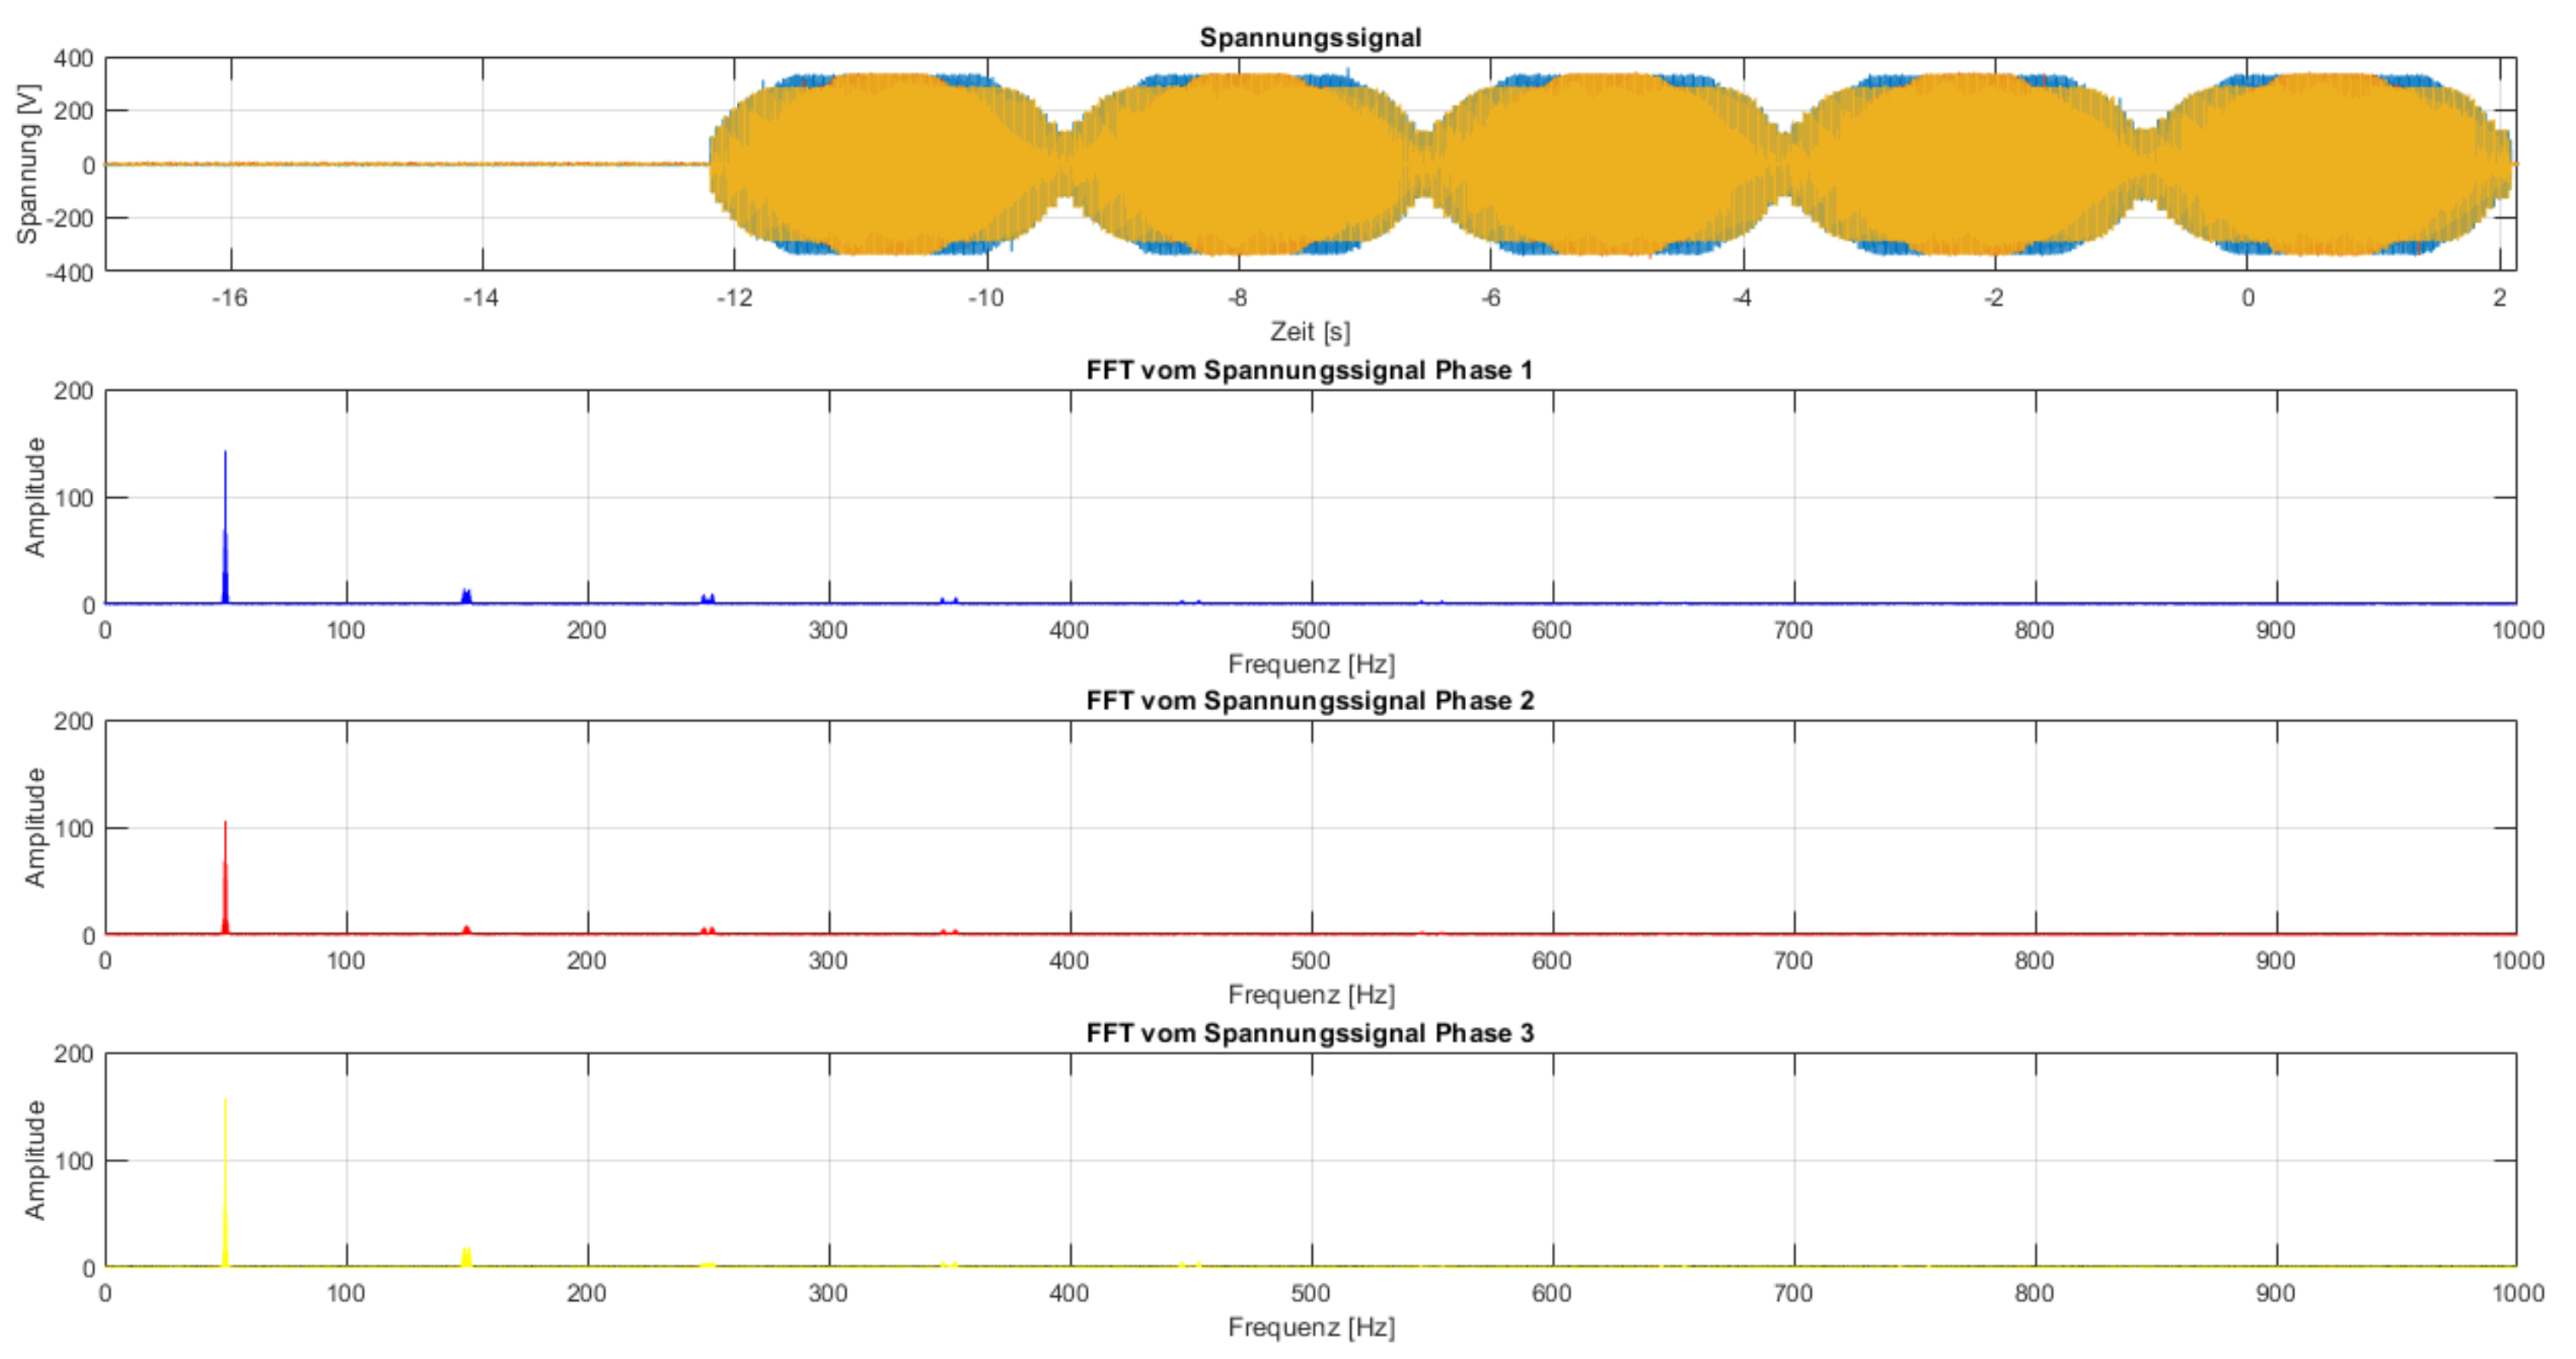
\includegraphics[width=\textwidth]{Mess_2Thyristoren_Widerstand_AufAbFahren.png}	
	\caption{Messung mit dem harten Auf- und Absteuern und zwei Thyristoren}\label{Mess_2Thyristoren_Widerstand_AufAbFahren}	
\end{figure}

Visuell sieht das harte Auf- und Absteuern mit der Sparvariante fast gleich aus wie die mit den drei angesteuerten Thyristoren auf der Abbildung \ref{fig:Mess_Sanft}. Jedoch beim Betrachten des FFTs zeigen sich grosse Unterschiede. Die Werte der Amplituden bei verschiedenen Frequenzen sind auf der Tabelle \ref{tab:Mess_2Thyristoren_Spannung_Widerstand_AufAb_hart} aufgelistet.

\newpage
\begin{table}[ht!]
	\centering
	\begin{tabular}{|l|l|l|l|}
		\hline
		Frequenz {[}Hz{]} & Amplitude Phase 1 {[}V{]}                                                           & Amplitude Phase 2 {[}V{]}                                                           & Amplitude Phase 3 {[}V{]}                                                           \\ \hline
		49.65             & 68.8653                                                                             & 68.5665                                                                             & 57.1292                                                                             \\ \hline
		49.95             & 67.5597                                                                             & 50.5713                                                                             & 74.4293                                                                             \\ \hline
		50                & 142.7445                                                                            & 105.9402                                                                            & 157.2093                                                                            \\ \hline
		50.05             & 35.291                                                                              & 26.4882                                                                             & 38.8518                                                                             \\ \hline
		50.35             & 65.3531                                                                             & 65.6359                                                                             & 51.887                                                                              \\ \hline
		149.65            & 9.7876                                                                              & 2.7987                                                                              & 11.8526                                                                             \\ \hline
		150               & 8.3874                                                                              & 8.3817                                                                              & 7.6543                                                                              \\ \hline
		150.35            & 11.1326                                                                             & 2.5768                                                                              & 12.4114                                                                             \\ \hline \hline
		Frequenz {[}Hz{]} & \begin{tabular}[c]{@{}l@{}}Verhältnis zur \\ Grundschwingung\\ Phase 1\end{tabular} & \begin{tabular}[c]{@{}l@{}}Verhältnis zur \\ Grundschwingung\\ Phase 2\end{tabular} & \begin{tabular}[c]{@{}l@{}}Verhältnis zur \\ Grundschwingung\\ Phase 3\end{tabular} \\ \hline
		49.65             & 48.24\%                                                                             & 64.7\%                                                                              & 36.34\%                                                                             \\ \hline
		49.95             & 47.32\%                                                                             & 47.74\%                                                                             & 47.34\%                                                                             \\ \hline
		50                & 100\%                                                                               & 100\%                                                                               & 100\%                                                                               \\ \hline
		50.05             & 24.72\%                                                                             & 25\%                                                                                & 24.7\%                                                                              \\ \hline
		50.35             & 45.78\%                                                                             & 61.96\%                                                                             & 33\%                                                                                \\ \hline
		149.65            & 6.86\%                                                                              & 2.64\%                                                                              & 7.54\%                                                                              \\ \hline
		150               & 5.88\%                                                                              & 7.9\%                                                                               & 4.87\%                                                                              \\ \hline
		150.35            & 7.8\%                                                                               & 2.43\%                                                                              & 7.9\%                                                                               \\ \hline
	\end{tabular}
\caption{Amplitudenwerte bei der Frequenzen mit zwei Thyristoren bei hartem Auf- und Absteuern}\label{tab:Mess_2Thyristoren_Spannung_Widerstand_AufAb_hart}
\end{table}

Der Vergleich der verschiedenen Phasen zeigt auf, dass die Phasen unterschiedlich belastet sind. Erstmals tritt bei den Messungen die dritte Harmonische auf. Die Auswirkungen dieser Harmonische ist im Kapitel \todo{Kapitel 3te Harmonische} aufgezeigt. Es entstehen bei den Amplituden Unterschiede von fast 30\% zwischen den verschiedenen Phasen auf. 



\newpage
\subsubsection*{Sanftes Auf- und Absteuern}

\begin{figure}[ht!]
	\centering
	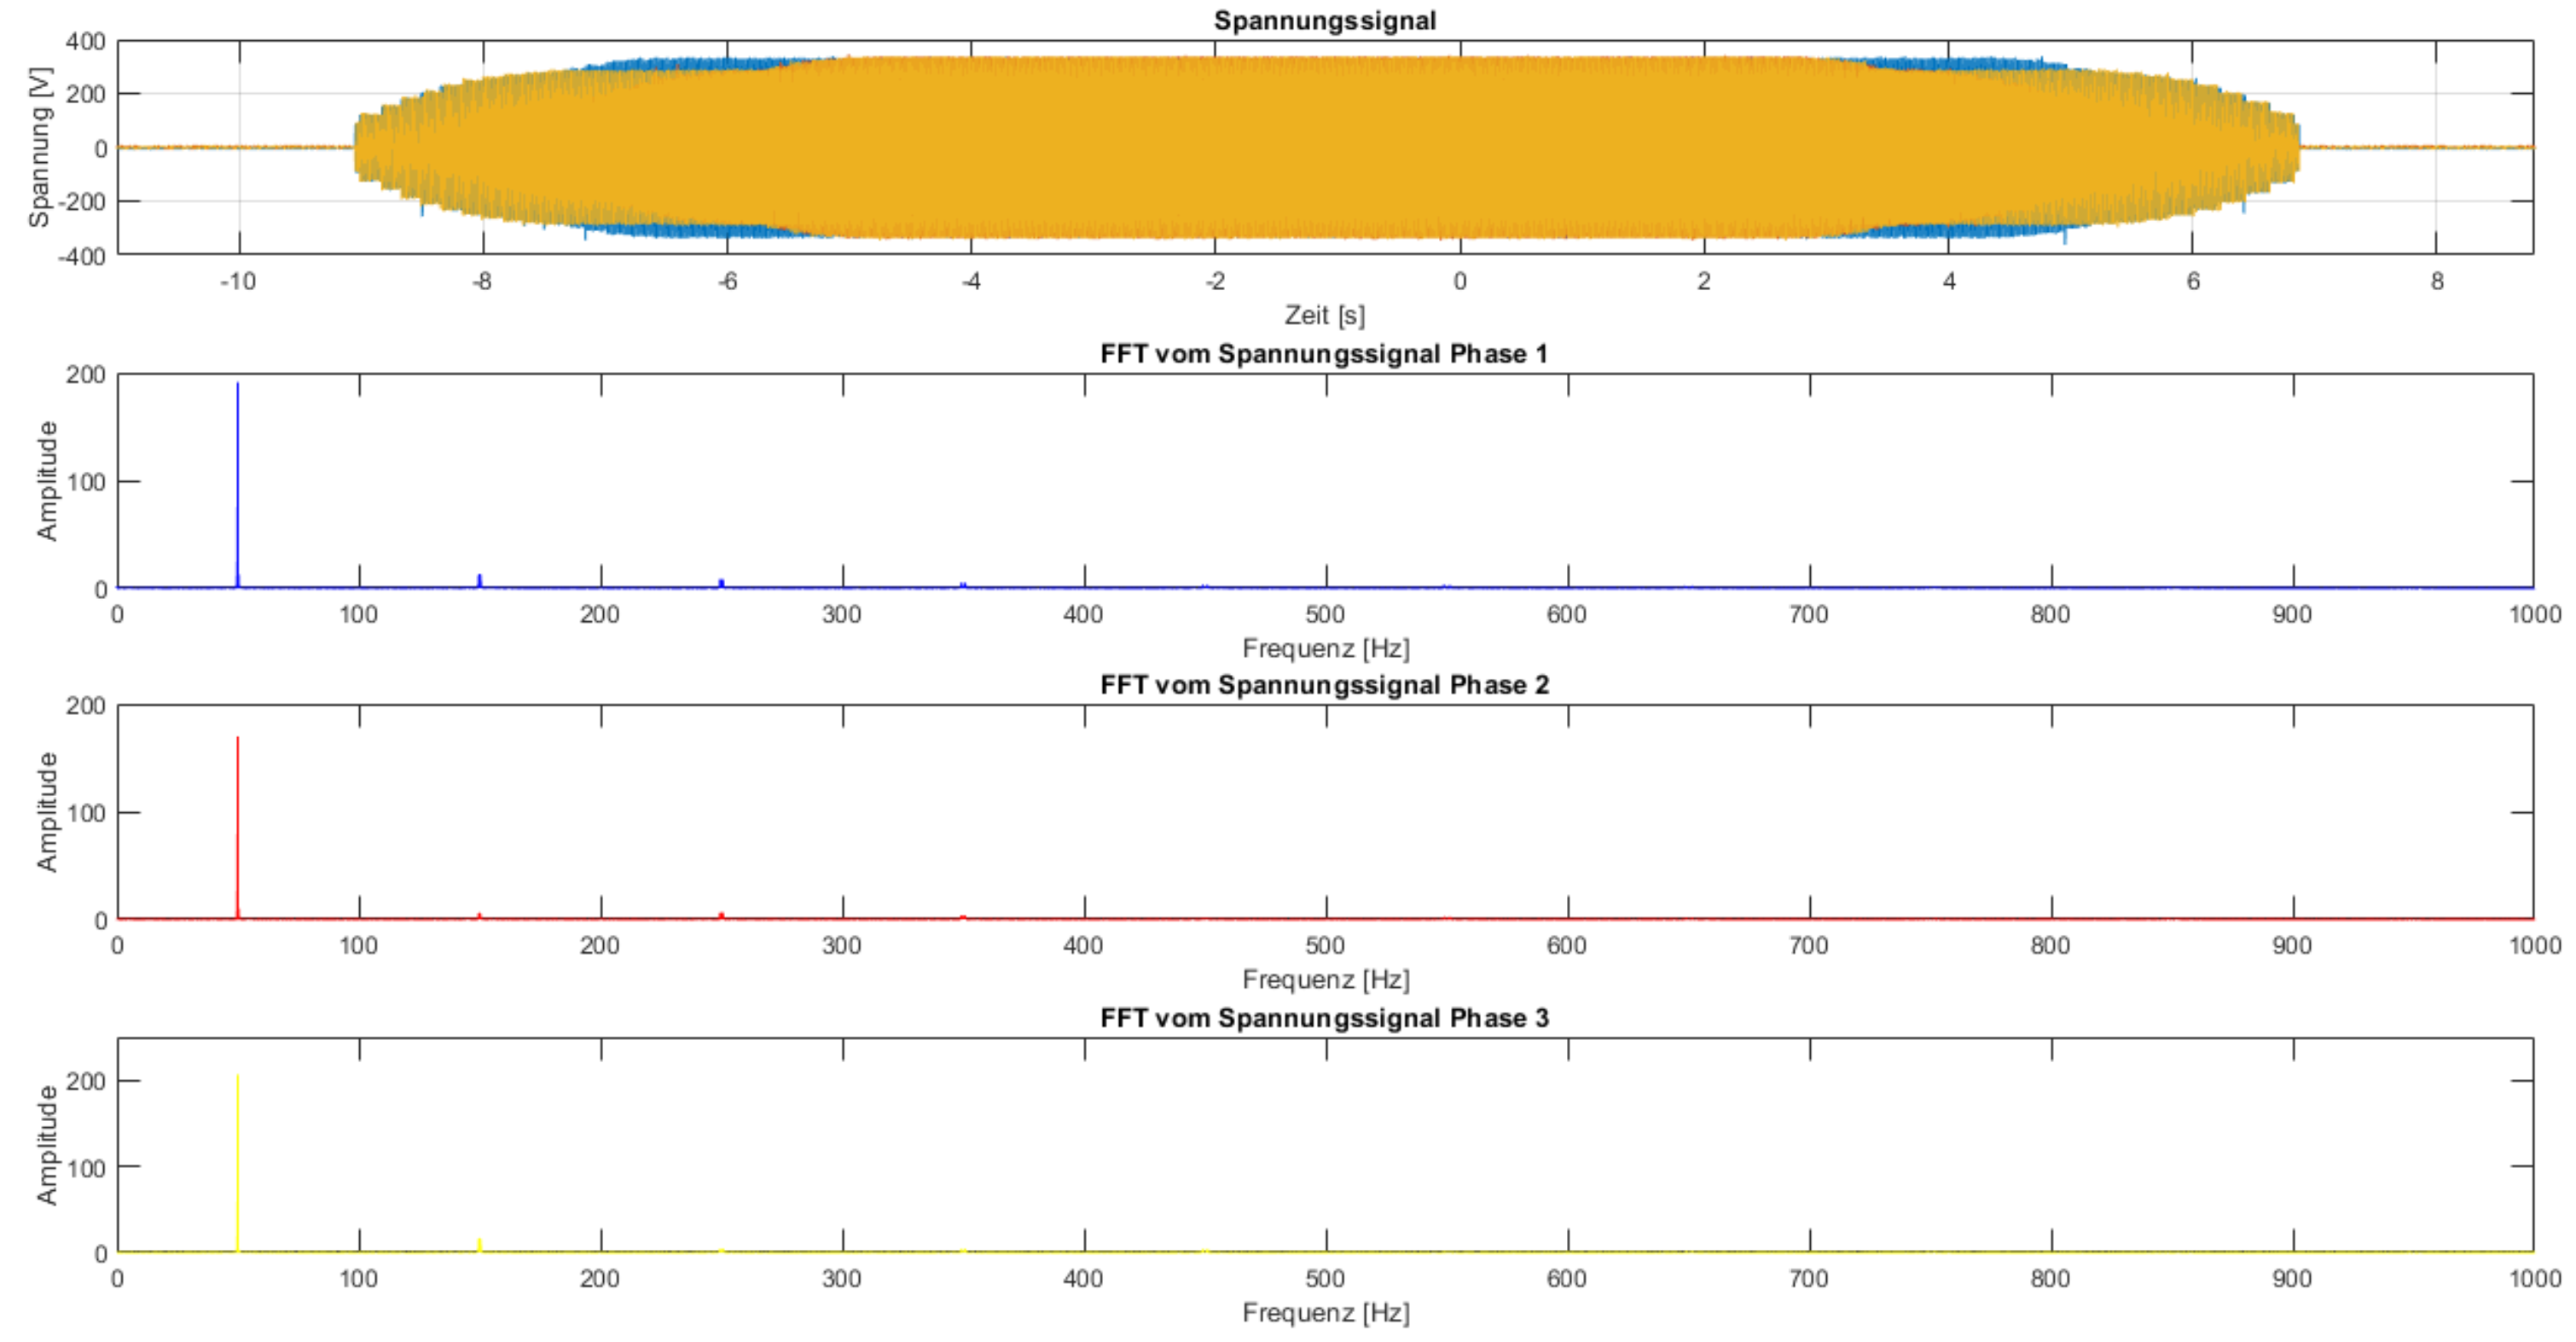
\includegraphics[width=\textwidth]{Mess_2Thyristoren_Widerstand_AufAbFahren_langsam.png}	
	\caption{Messung mit dem sanften Auf- und Absteuern und zwei Thyristoren}\label{fig:Mess_2Thyristoren_Widerstand_AufAbFahren_langsam}	
\end{figure}

Wie auch beim hartem Auf- und Absteuern, sehen die Spannungsverläufe auf der Abbildung \ref{fig:Mess_2Thyristoren_Widerstand_AufAbFahren_langsam} visuell sehr ähnlich auch das sanfte Auf- und Absteuern mit drei Thyristoren auf der Abbildung \ref{Mess_1Thyristoren_Widerstand_AufAbFahren_langsam}. Einziger Unterschied ist, das beim Hoch- und Runterfahren die drei Phasen nicht alle gleich hoch sind. Dies resultiert in einem FFT mit unterschiedlichen Amplitudenhöhen für die verschiedenen Phasen. Die Werte des FFTs sind in der Tabelle \ref{tab:Mess_2Thyristoren_Spannung_ASM_AufAb_sanft} aufgelistet. 

\newpage
\begin{table}[ht!]
	\centering
	\begin{tabular}{|l|l|l|l|}
		\hline
		Frequenz {[}Hz{]} & Amplitude Phase 1 {[}V{]}                                                           & Amplitude Phase 2 {[}V{]}                                                           & Amplitude Phase 3 {[}V{]}                                                           \\ \hline
		49.9              & 38.5998                                                                             & 19.6499                                                                             & 34.7131                                                                             \\ \hline
		49.95             & 77.5993                                                                             & 82.1127                                                                             & 60.2946                                                                             \\ \hline
		50                & 191.1857                                                                            & 169.7545                                                                            & 206.7036                                                                            \\ \hline
		50.05             & 125.8716                                                                            & 123.6057                                                                            & 126.0935                                                                            \\ \hline
		50.1              & 42.6127                                                                             & 17.4015                                                                             & 26.3464                                                                             \\ \hline
		149.8             & 12.7189                                                                             & 3.9393                                                                              & 16.14                                                                               \\ \hline
		150               & 2.6765                                                                              & 4.3294                                                                              & 5.5055                                                                              \\ \hline
		150.2             & 9.6611                                                                              & 5.9313                                                                              & 13.152                                                                              \\ \hline \hline
		Frequenz {[}Hz{]} & \begin{tabular}[c]{@{}l@{}}Verhältnis zur \\ Grundschwingung\\ Phase 1\end{tabular} & \begin{tabular}[c]{@{}l@{}}Verhältnis zur \\ Grundschwingung\\ Phase 2\end{tabular} & \begin{tabular}[c]{@{}l@{}}Verhältnis zur \\ Grundschwingung\\ Phase 3\end{tabular} \\ \hline
		49.9              & 20.19\%                                                                             & 11.58\%                                                                             & 16.79\%                                                                             \\ \hline
		49.95             & 40.59\%                                                                             & 48.37\%                                                                             & 29.17\%                                                                             \\ \hline
		50                & 100\%                                                                               & 100\%                                                                               & 100\%                                                                               \\ \hline
		50.05             & 65.84\%                                                                             & 72.81\%                                                                             & 61\%                                                                                \\ \hline
		50.1              & 22.29\%                                                                             & 10.25\%                                                                             & 12.75\%                                                                             \\ \hline
		149.8             & 6.65\%                                                                              & 2.32\%                                                                              & 7.81\%                                                                              \\ \hline
		150               & 1.4\%                                                                               & 2.55\%                                                                              & 2.66\%                                                                              \\ \hline
		150.2             & 5.05\%                                                                              & 3.49\%                                                                              & 6.36\%                                                                              \\ \hline
	\end{tabular}
\caption{Amplitudenwerte bei der Frequenzen mit zwei Thyristoren bei sanftem Auf- und Absteuern}\label{tab:Mess_2Thyristoren_Spannung_Widerstand_AufAb_sanft}
\end{table}


Bei dem Peak der Grundschwingung gibt es eine Abweichung von fast 10\% zwischen den drei Phasen. Dies ist auch bei den anderen Frequenzen der Fall, im Verhältnis zur Grundschwngung der jeweiligen Phase. Einzig bei der dritten Harmonischen ist die Abweichung relativ wenig mit 1.22\%. 

\newpage
\subsubsection{Sparvariante mit der ASM und zwei Thyristoren}
Bei der Ansteuerung der ASM eignet sich das harte Auf- und Absteuern nicht, deshalb wird nur das sanfte Auf- und Absteuern aufgezeigt.
\subsubsection*{Sanftes Auf- und Absteuern}
\begin{figure}[ht!]
	\centering
	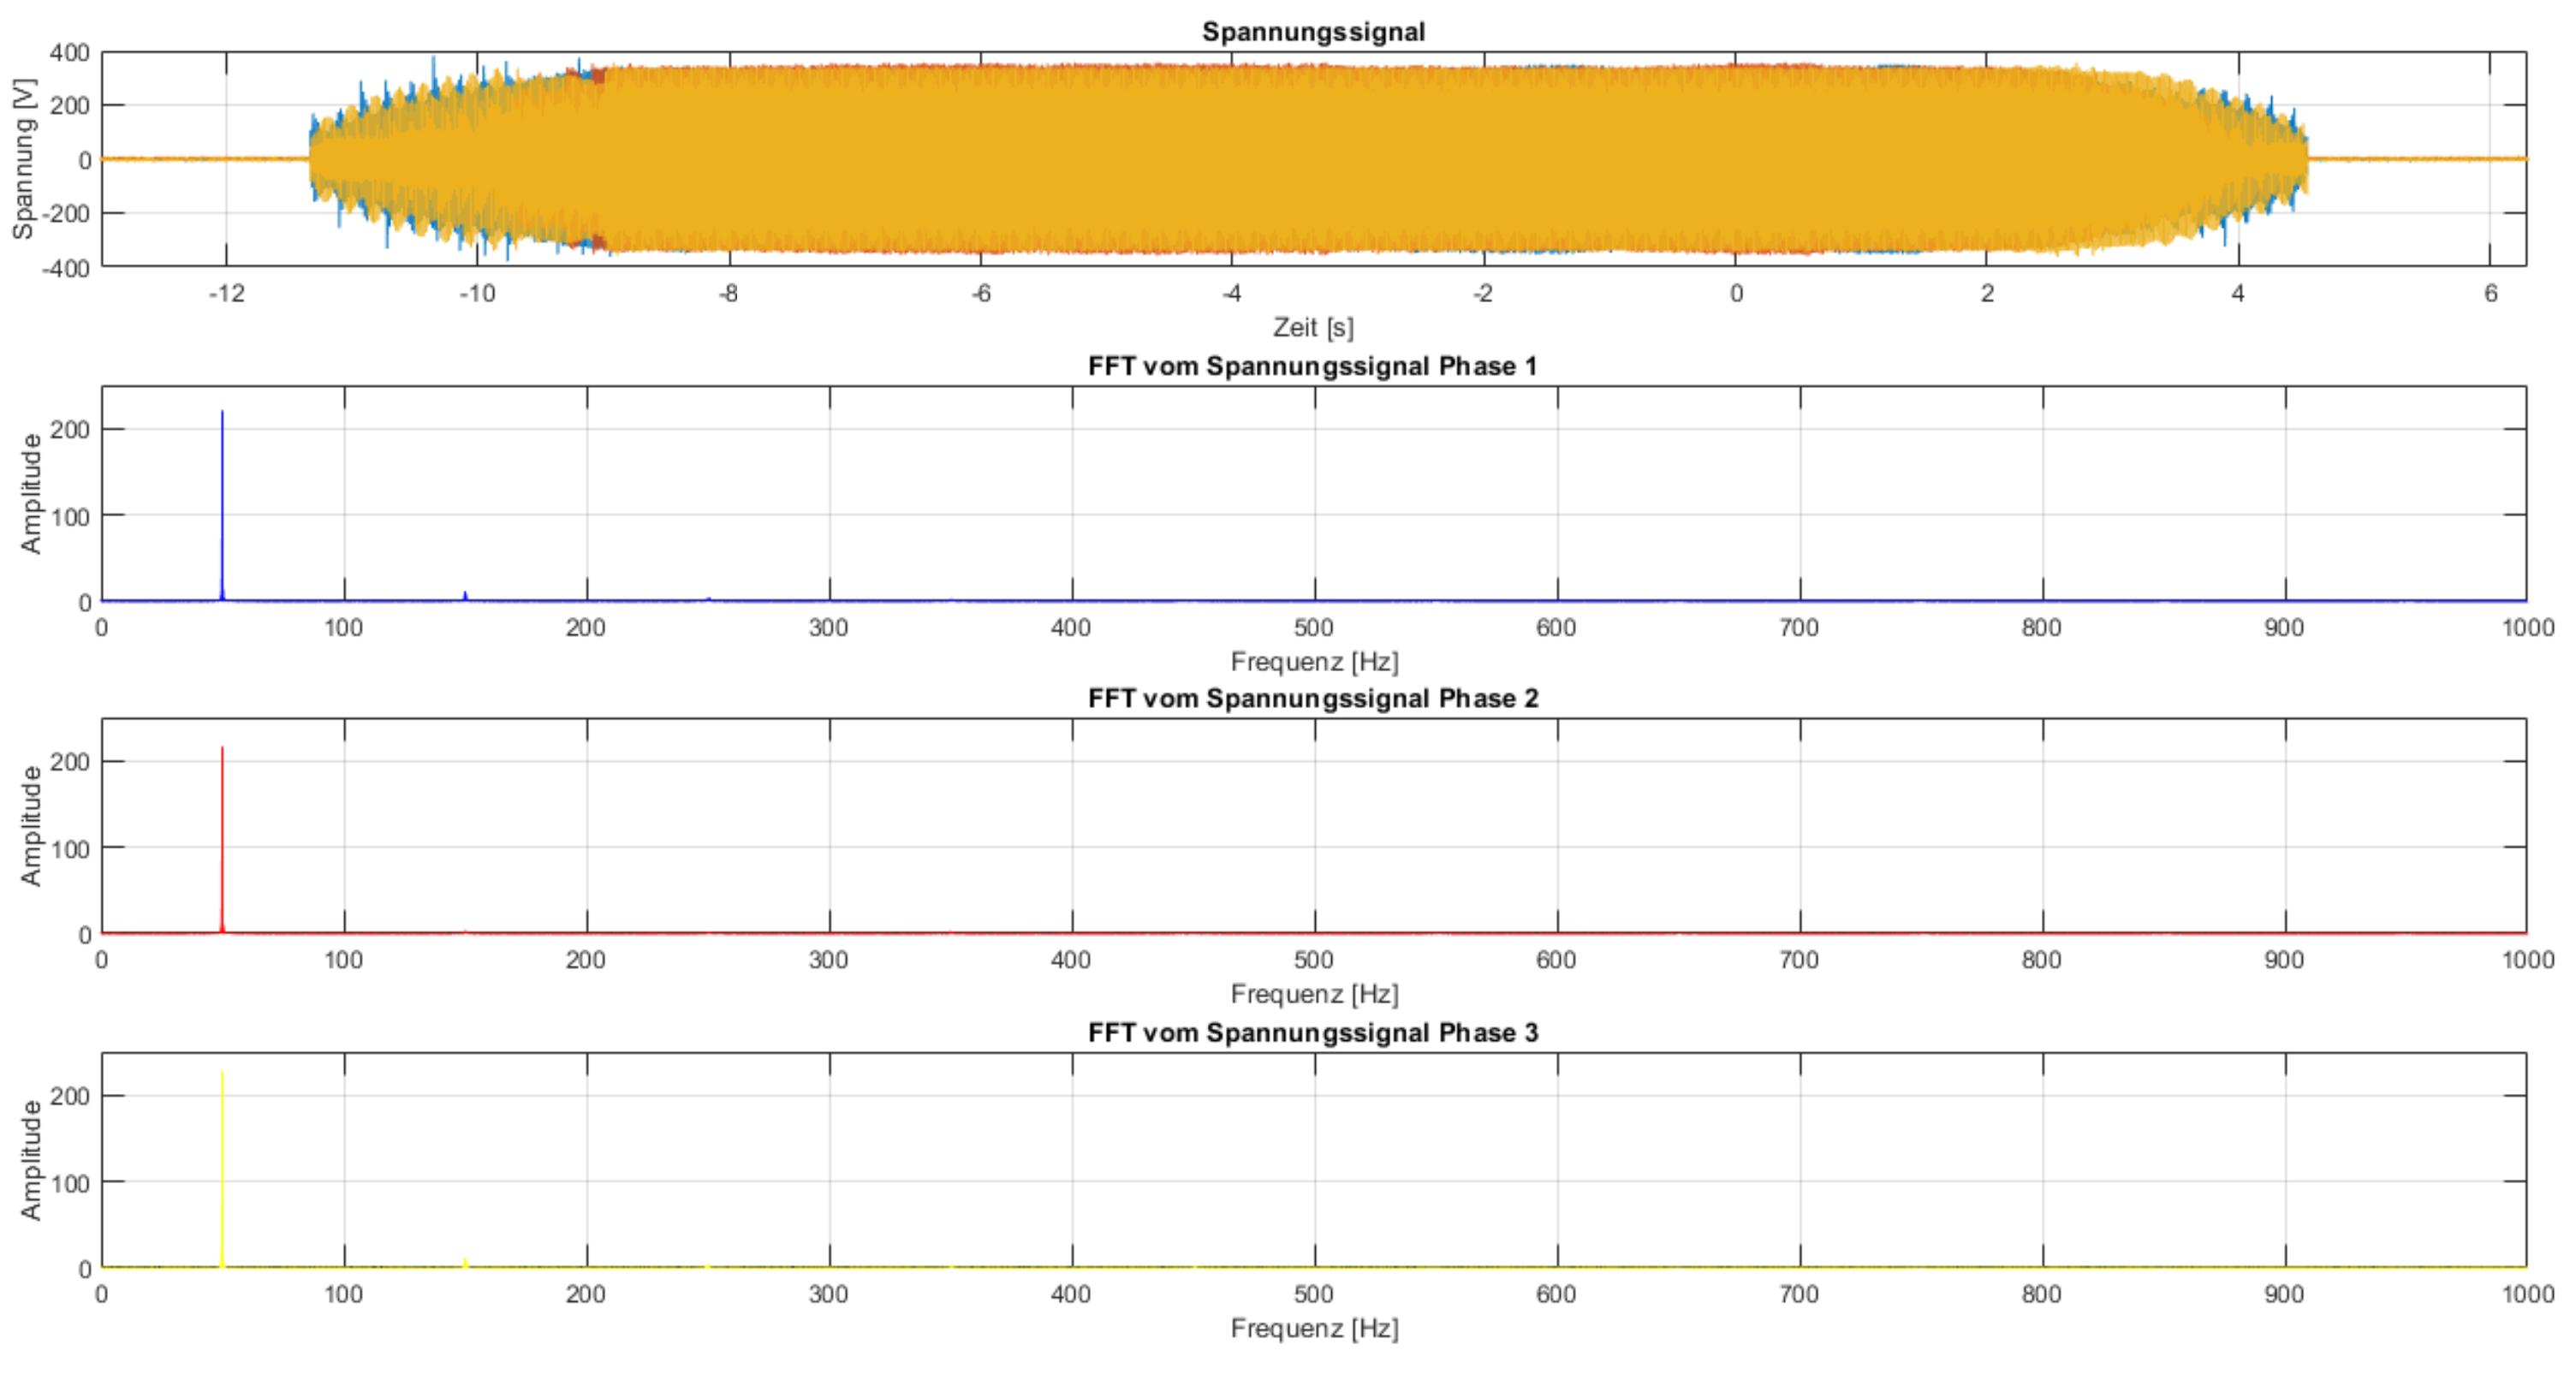
\includegraphics[width=\textwidth]{Mess_ASM_2Thyristoren_AufAb_langsam.png}	
	\caption{Messung mit dem sanften Auf- und Absteuern und zwei Thyristoren}\label{fig:Mess_2Thyristoren_ASM_AufAbFahren_langsam}	
\end{figure}

Anders als bei den beiden Sparvariante mit dem Widerstand, zeigen sich bei der Sparvariante mit der ASM auf der Abbildung \ref{fig:Mess_2Thyristoren_ASM_AufAbFahren_langsam} im Vergleich zum sanftem Auf- und Absteuern mit drei Thyristoren auf der Abbildung \ref{fig:Mess_ASM_Sanft_langsam} bereits visuelle Unterschiede. So sieht das Hoch- und Runterfahren bei der Sparvariante linearer aus als beim Betrieb mit drei Thyristoren. Bei der Sparvariante mit der ASM und zwei Thyristoren treten ebenfalls Unterschiede zwischen den FFTs der verschiedenen Phasen auf, diese sind in der Tabelle \ref{tab:Mess_2Thyristoren_Spannung_ASM_AufAb_sanft} aufgeführt. 

\newpage
\begin{table}[ht!]
	\centering
	\begin{tabular}{|l|l|l|l|}
		\hline
		Frequenz {[}Hz{]} & Amplitude Phase 1 {[}V{]}                                                           & Amplitude Phase 2 {[}V{]}                                                           & Amplitude Phase 3 {[}V{]}                                                           \\ \hline
		49.9              & 37.5857                                                                             & 42.9618                                                                             & 47.1945                                                                             \\ \hline
		49.95             & 75.5033                                                                             & 87.0174                                                                             & 77.0178                                                                             \\ \hline
		50                & 220.7586                                                                            & 216.2571                                                                            & 227.9957                                                                            \\ \hline
		50.05             & 111.631                                                                             & 110.0439                                                                            & 102.3768                                                                            \\ \hline
		50.1              & 44.4045                                                                             & 65.6359                                                                             & 40.8044                                                                             \\ \hline
		149.95            & 6.9369                                                                              & 2.1636                                                                              & 5.8686                                                                              \\ \hline
		150               & 11.5575                                                                             & 1.4866                                                                              & 10.115                                                                              \\ \hline
		150.05            & 6.7811                                                                              & 2.7637                                                                              & 6.5154                                                                              \\ \hline \hline
		Frequenz {[}Hz{]} & \begin{tabular}[c]{@{}l@{}}Verhältnis zur \\ Grundschwingung\\ Phase 1\end{tabular} & \begin{tabular}[c]{@{}l@{}}Verhältnis zur \\ Grundschwingung\\ Phase 2\end{tabular} & \begin{tabular}[c]{@{}l@{}}Verhältnis zur \\ Grundschwingung\\ Phase 3\end{tabular} \\ \hline
		49.9              & 17.03\%                                                                             & 19.46\%                                                                             & 20.7\%                                                                              \\ \hline
		49.95             & 34.2\%                                                                              & 39.42\%                                                                             & 33.78\%                                                                             \\ \hline
		50                & 100\%                                                                               & 100\%                                                                               & 100\%                                                                               \\ \hline
		50.05             & 50.57\%                                                                             & 49.85\%                                                                             & 44.9\%                                                                              \\ \hline
		50.1              & 20.11\%                                                                             & 29.73\%                                                                             & 17.9\%                                                                              \\ \hline
		149.95            & 3.16\%                                                                              & 0.98\%                                                                              & 2.57\%                                                                              \\ \hline
		150               & 5.24\%                                                                              & 0.67\%                                                                              & 4.44\%                                                                              \\ \hline
		150.05            & 3.07\%                                                                              & 1.25\%                                                                              & 2.86\%                                                                              \\ \hline
	\end{tabular}
\caption{Amplitudenwerte bei der Frequenzen mit zwei Thyristoren bei sanftem Auf- und Absteuern}\label{tab:Mess_2Thyristoren_Spannung_ASM_AufAb_sanft}
\end{table}

Im Vergleich zu den Werten des FFTs bei dem sanften Auf- und Absteuern mit drei Thyristoren in der Tabelle \ref{tab:Mess_Spannung_ASM_AufAb_sanft}, ist ersichtlich, dass die Peaks des Trägerbandes um \SI{50}{Hz} im Verhältnis zur Grundschwingung bei der Sparvariante kleiner sind, als bei der Ansteuerung mit drei Thyristoren. Ein weiterer Unterschied ist die dritte Harmonische, welche nur bei der Sparvariante vorkommt. 


\newpage
\subsection{Leistungsfaktor}
Um den Leistungsfaktor für den Phasenanschnitt zu berechenen können die Formeln im Kapitel \ref{sec:Leistungsfaktor} benutzt werden. Jedoch funktioniert diese Formeln bei der Kombination der verschiedenen Verfahren oder mit dem Hochfahren durch den Phasenanschnitt nicht. Mit folgender Formel kann der Leistungsfaktor ebenfalls berechnet werden:
\begin{equation}
\lambda = \frac{P}{S}
\end{equation}
Um die Wirkleistung zu erhalten, können die Strom- und Spannungswerte multipliziert werden:
\begin{equation}
P = u(t) \cdot i(t)
\end{equation}
Für die Scheinleistung müssen die Effektivwerte der Spannung und des Stromes multipliziert werden:
\begin{equation}
S = U_{rms} \cdot I_{rms}
\end{equation}
Wobei der Effektivwert des Stromes und der Spannung über die gesamte Zeitdauer berechnet wurde. Der Matlabcode dieser Berechnungen befindet sich im Anhang im Kapitel \ref{sec:Leistungsfaktor_Messungen}. 

Die Resultate der Leistungsfaktorberechnungen sind in der Tabelle \ref{tab:Leistungsfaktor_ASM_Widerstand} aufgeführt.

\begin{table}[ht!]
	\centering
	\begin{tabular}{|l|l|}
		\hline
		Ansteuerungsart ASM                                   		& Leistungsfaktor \\ \hline 
		Sanftes Auf- und Absteuern                          		& 0.2947          \\ \hline
		Sanftes Auf- und Absteuern mit 150$\Omega$ Vorwiderstand 	& 0.3493          \\ \hline
		Phasenanschnitt 90\textdegree                               & 0.4879          \\ \hline
		Phasenanschnitt 60\textdegree                               & 0.4155          \\ \hline \hline
		Ansteuerungsart Widerstand                            		& Leistungsfaktor \\ \hline 
		Sanftes Auf- und Absteuern                          		& 0.9987          \\ \hline
		Hartes Auf- und Absteuern                                   & 0.9988          \\ \hline
		Phasenanschnitt 90\textdegree                         		& 0.9953          \\ \hline
		Phasenanschnitt 60\textdegree                         		& 0.999           \\ \hline
	\end{tabular}
\caption{Leistungsfaktor mit verschiedenen Ansteuerungsverfahren bei der ASM und dem Widerstand}\label{tab:Leistungsfaktor_ASM_Widerstand}
\end{table}
Bei der ASM im Leerlauf gilt, je näher der Leistungsfaktor bei 0 ist desto besser. Da der Leistungsfaktor das Verhältnis von Wirk- zu Scheinleistung ist und sich die Maschine im Leerlauf befindet, wird die Wirkleistung nur für die Ummagnetisierungs- und Eisenverluste benötigt. Wenn der Leistungsfaktor höher ist, heisst dies, dass mehr Verlustleistung entsteht. Um dies zu beweisen wurde ein Vorwiderstand mit \SI{150}{\Omega} in den Stromkreis geschaltet. Dabei konnte festgestellt werden, dass sich wie erwartet mit dem Vorwiderstand der Leistungsfaktor erhöht, da zusätzlich Wirkleistung im Widerstand verheizt wird. Wenn der Leistungsfaktor der verschiedenen Ansteuerungsarten analysiert werden, kann klar gesagt werden, dass sich das sanfte Auf- und  Absteuern am besten eignet für die ASM.

Bei Ohmschen Lasten gilt jedoch, je näher der Leistungsfaktor bei 1 ist, desto besser. Bei den Messungen mit den verschiedenen Ansteuerungsarten wurde festgestellt, dass der Leistungsfaktor beim Phasenanschnitt mit einem Winkel von 60\textdegree \hspace{0.02cm} am höchsten ist. Jedoch verbietet die Normen den Gebrauch des Phasenanschnittes mit den Winkeln von 90\textdegree \hspace{0.02cm} wegen den erhöhten Werten der Amplituden. Deshalb macht es Sinn nur das sanfte und harte Auf- und Abfahren zu vergleichen. Bei diesen zwei Ansteuerungsverfahren hat das harte Auf- und Absteuern einen höheren Leistungsfaktor. Jedoch ist der Unterschied von 0.0001 sehr klein und kann praktisch vernachlässigt werden.
 



%\subsubsection{Schwingungspaketsteuerung mit Last in Stern}
%Für die Messung mit der Schwingungspaketsteuerung wurde eine Einschaltzeit von 0.5 Sekunden und eine Ausschaltzeit von 0.2 Sekunden gewählt. Die Ausschaltzeit darf nicht kürzer sein, da die Spannungsverstärkerschaltung und den Thyristorsteller eine Zeitverzögerung darstellen und so die Spannung nicht sofort ein- oder ausgeschaltet wird. Wenn die Ausschaltzeit kürzer ist, geht die Spannung zwischen den Paketen nicht auf \SI{0}{V}. 
%\begin{figure}[ht!]
%	\centering
%	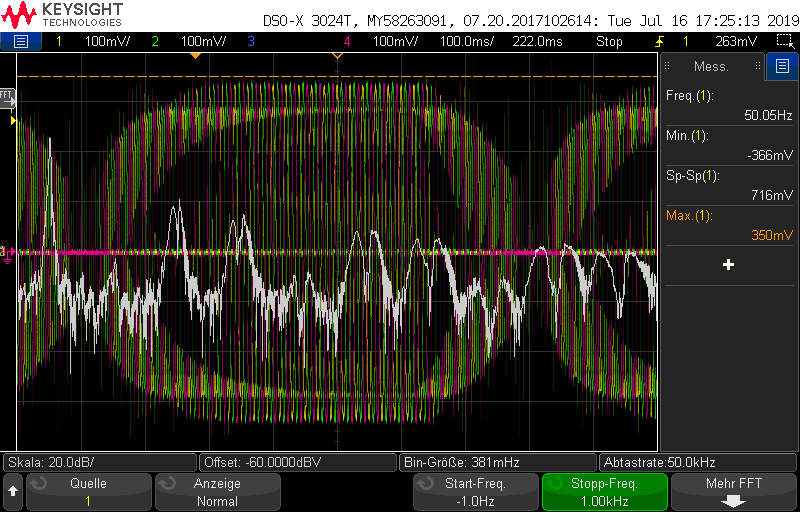
\includegraphics[width=0.7\textwidth]{Schwingungspaket_kurz.png}	
%	\caption{Das Spannungssignal aller Phasen bei Schwingungspaketsteuerung mit FFT}\label{fig:Mess_Schwing_kurz}
%\end{figure}
%
%Das FFT zeigt entgegen den Erwartungen aus der Theorie fast keine Subharmonische auf. Dafür sind Harmonische und Zwischehamrnische sehr ausgeprägt. Sehr gut zu sehen ist die Grundfrequenz von \SI{50}{Hz}, der erste Peak von der linken Seite. Dies ist darauf zurückzuführen, dass nicht direkt ein- und ausgeschaltet wird und so einem Sanft-Anlass ähnelt. Dies dominiert gegenüber dem harten Ein- und Ausschalten, welches die Subharmonische hervorrufen würde.
%\newpage
%\subsection{Phasenanschnittsteuerung mit 2 Thyristoren mit Last in Stern}
%Für die Sparansteuerung wurde ein Winkel von 90\textdegree \hspace{0.02cm} gewählt. 
%
%\begin{figure}[ht!]
%	\centering
%	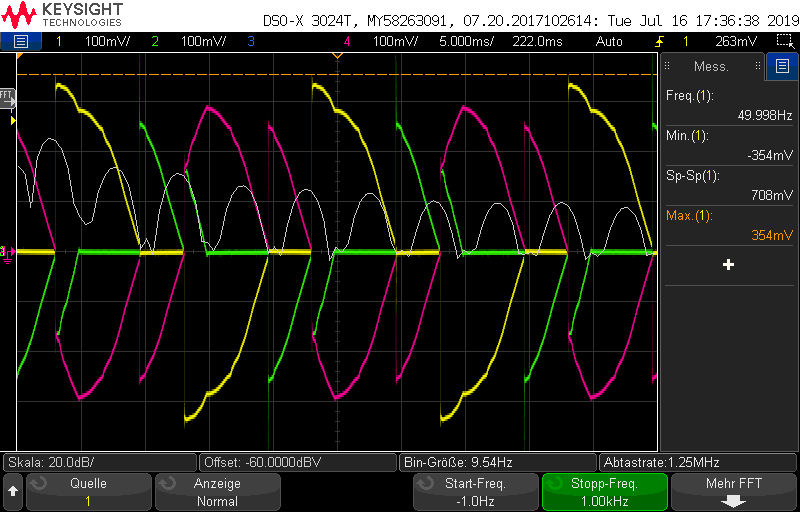
\includegraphics[width=0.7\textwidth]{2phas_90grad_kurz.png}	
%	\caption{Das Spannungssignal aller Phasen bei Schwingungspaketsteuerung mit FFT}\label{fig:Mess_2phas_kurz}
%\end{figure}
%
%
%\subsection{Phasenanschnittsteuerung mit 1 Thyristor mit Last in Stern}
%Für die Sparansteuerung wurde ein Winkel von 90\textdegree gewählt. 
%
%\begin{figure}[ht!]
%	\centering
%	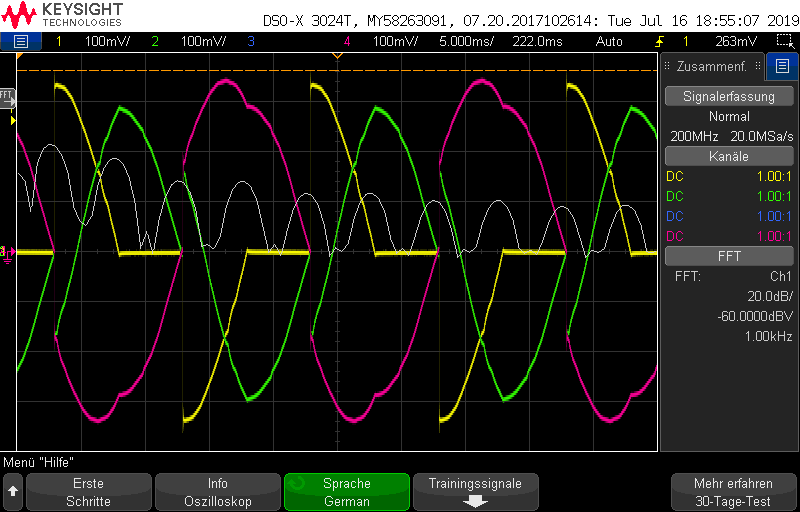
\includegraphics[width=0.7\textwidth]{1phas_90grad_kurz.png}	
%	\caption{Das Spannungssignal aller Phasen bei Schwingungspaketsteuerung mit FFT}\label{fig:Mess_1phas_kurz}
%\end{figure}




